\documentclass[12pt,a4paper]{article}
\usepackage[utf8]{inputenc}
\usepackage{amsmath}
\usepackage{amsfonts}
\usepackage{amssymb}
\usepackage[top=3cm, bottom=2cm, left=3cm, right=2cm]{geometry} % geometria da pagina
\usepackage{natbib} 			% Fazer referencias bibliograficas
\usepackage{graphicx}
\graphicspath{{figuras/}}
\usepackage{macrosfabbri}
\usepackage{indentfirst}
%\usepackage{url}
\usepackage{hyperref}

%comandos criados por David
\newcommand{\bpi}{\boldsymbol{\pi}}
\newcommand{\y}{{\bf y}}
\newcommand{\C}{{\bf C}}

\begin{document}

\tableofcontents
\newpage

\newpage
%\pagestyle{headings}
%\section{Introdução}
\noindent{\bf INTRODUÇ\~AO}\\

A Visão Computacional é uma área de pesquisa que se ocupa em utilizar imagens em 2D de um cenário, obtidas de uma ou mais câmeras digitais para produzir uma construção virtual em 3D, ou extrair qualquer outro tipo de informação útil como o cruzamento de informações entre imagens. A captação da geometria 3D de um cenário a partir de imagens produzidas por câmeras, analisando a disparidade entre elementos correspondentes nessas imagens, é chamada de visão {\it estereoscópica}, da qual a visão computacional se utiliza para desenvolver modelos adequados à descrição geométrica tanto da cena 3D em questão como das câmeras que fazem a projeção da cena na imagem 2D.

\begin{figure}[!htb]
\centering
\caption{{\it O maior passo no uso de visão computacional em pesquisas interplanetárias foi dado na missão NASA/JPL Mars Exploration Rover (MER).}}
\begin{tabular}{l}
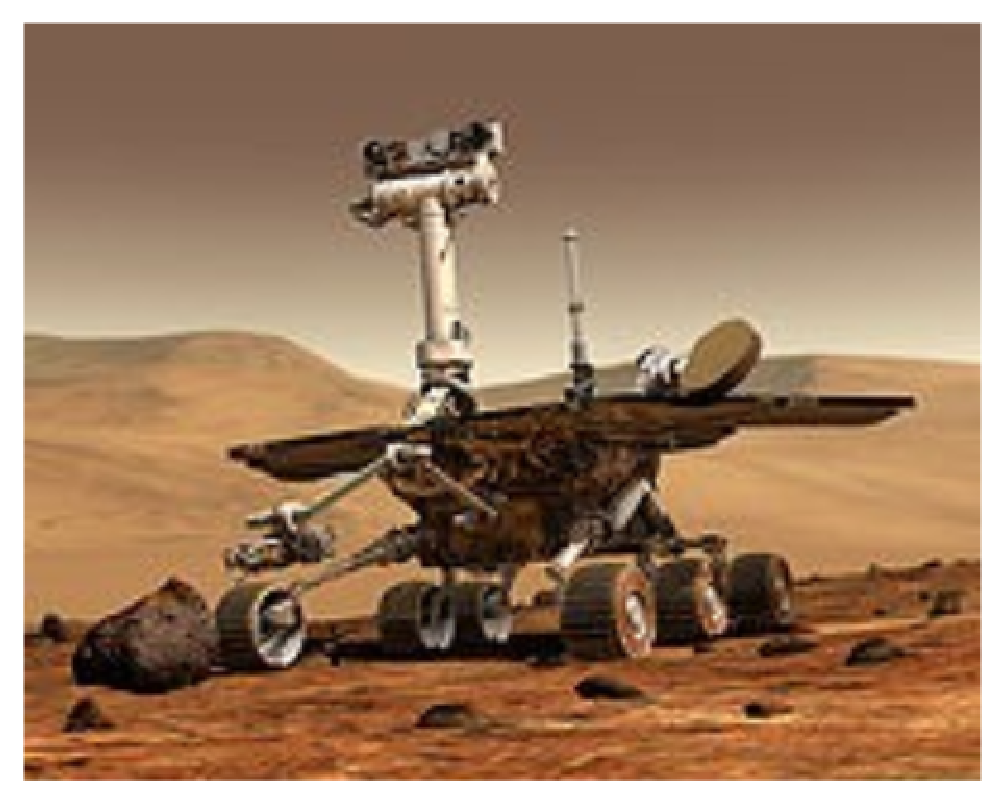
\includegraphics[scale=.5]{mars-rover}\\ 
\small{Fonte: \citep{mars-rover}}\\ 
\end{tabular}
\label{fig.mars-rover}
\end{figure}

A geometria projetiva é a principal teoria matemática usada em visão computacional tridimensional. Com a introdução de algumas definições e conceitos, a geometria projetiva pode ser estudada em termos de álgebra linear, onde tal abordagem traz alguns benefícios de modelagem e é amplamente utilizada por pesquisadores dessa área, mas também possui algumas limitações. Em pesquisas mais recentes, verificou-se a eficácia do uso de técnicas de geometria algébrica em resoluções de sistemas de equações polinomiais, oriundos de problemas de visão computacional 3D. Mais recentemente ainda, \citep{tese-fabbri} introduziram uma abordagem em termos de geometria diferencial, onde é possível aplicar o cálculo diferencial trabalhando diretamente com as equações algébricas. Essa abordagem permite um maior poder de modelagem matemática e computacional do espaço tridimensional através das imagens.


\subsection*{Motivação}
As motivações para a pesquisa estão ligadas às suas aplicações em diversas áreas. A extração de informação da geometria 3D de um ambiente pode, por exemplo, ser utilizada na determinação da orientação e posição de veículos autônomos, para que os mesmos identifiquem a trajetória para os seus objetivos considerando a possibilidade de obstáculos. Um exemplo famoso, segundo \citep{mars-rover}, é a aplicação em pesquisas interplanetárias onde foram usados algoritmos de visão computacional em veículos de exploração de Marte (Mars Exploration Rover - MER, em inglês), observado na figura \ref{fig.mars-rover}.


Uma aplicação mais recente foi a reconstrução virtual de objetos, estátuas ou monumentos de valor histórico e cultural que tenham sido destruídos pela ação do tempo ou do homem (possivelmente em guerras), através da aquisição de imagens em acervos ou na internet. Um exemplo é o Museu de Mosul {\footnote{Outros exemplos podem ser encontrados em http://www.projectmosul.org/}}, no Iraque, atacado pelo 
Estado Islâmico em 2015, que teve algumas de suas obras reconstruídas como podemos visualizar na figura \ref{fig.mossul}.

\begin{figure}[!htb]
\centering
\subfloat{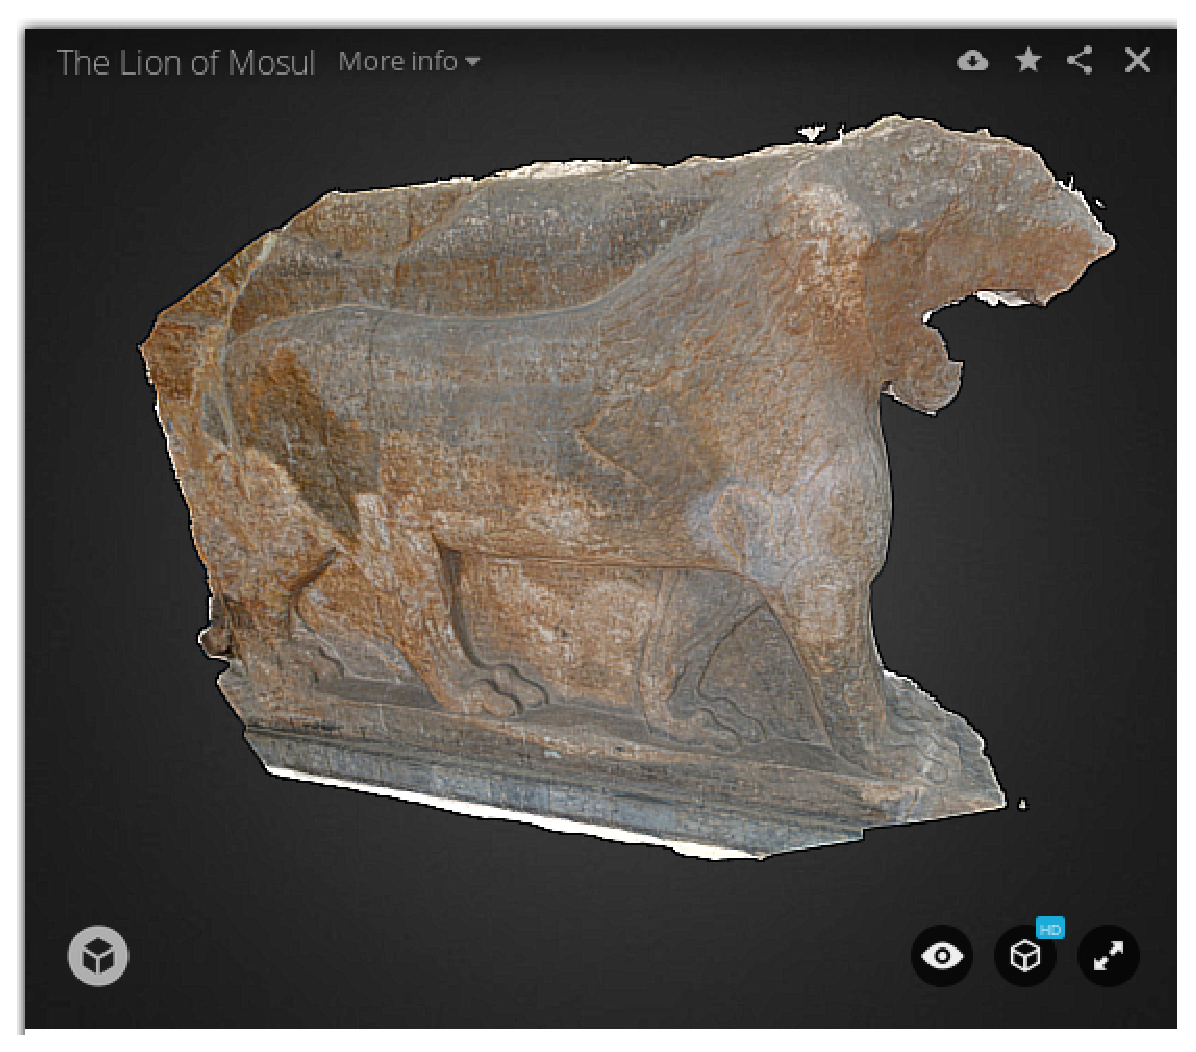
\includegraphics[scale=.385]{leao-mosul}}
\quad
\subfloat{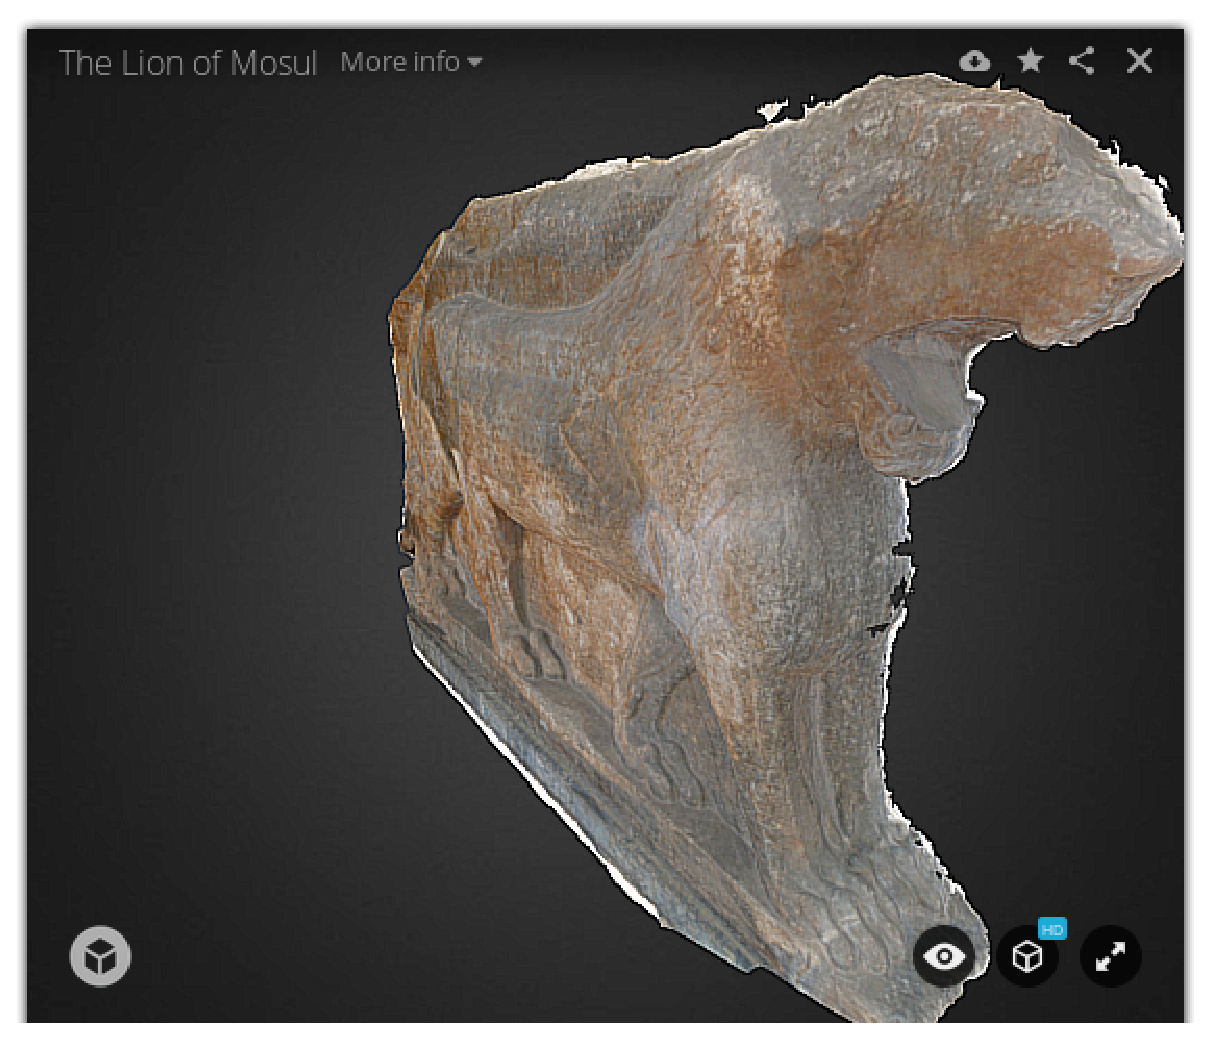
\includegraphics[scale=.385]{lion-mosul-2}}
\caption{{\it A reconstrução do Leão de Mosul, um dos artefatos destruídos por extremistas religiosos em 2015 no Iraque.}}
\label{fig.mossul}
\end{figure}

As aplicações de visão computacional são bastante variadas, com pesquisas em outras áreas como astronomia, medicina e química. Para se ter uma ideia, \citep{ballard-82} já apresentavam imagens e tabelas com resumos de aplicações em oito áreas diferentes no início dos anos 1980.  

Novos avanços em reconstrução 3D vêm sendo realizados constantemente como observamos em \cite{fabbri-drawing}, que apresentam uma abordagem para a reconstrução de um desenho 3D (3D \emph{drawing} em inglês) de uma cena. Isto é, um conjunto de fragmentos de curvas em 3D interligadas de forma que preserve suas relações espaciais, capturadas em forma de gráficos a partir de um grande conjunto de dados multifocal. A ideia base é aprimorar uma abordagem anterior (3D curve \emph{sketch}) divulgada pelos mesmos autores, \citep{fabbri-sketch}, conforme exemplo visualizado na figura \ref{fig.drawing2}.
%\begin{figure}[!htb]
%\centering
%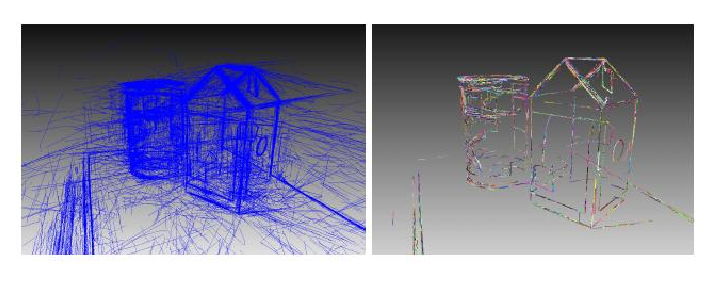
\includegraphics[scale=1.1]{3D-drawing}
%\caption{{\it Uma comparação visual: à esquerda os resultados com o 3D curve sketch e à direita os resultados após o aprimoramento com 3D drawing. Repare na redução significante de outliers sem prejuízo do esboço da superfície.}}
%\label{fig.drawing}
%\end{figure}

\begin{figure}
\centering
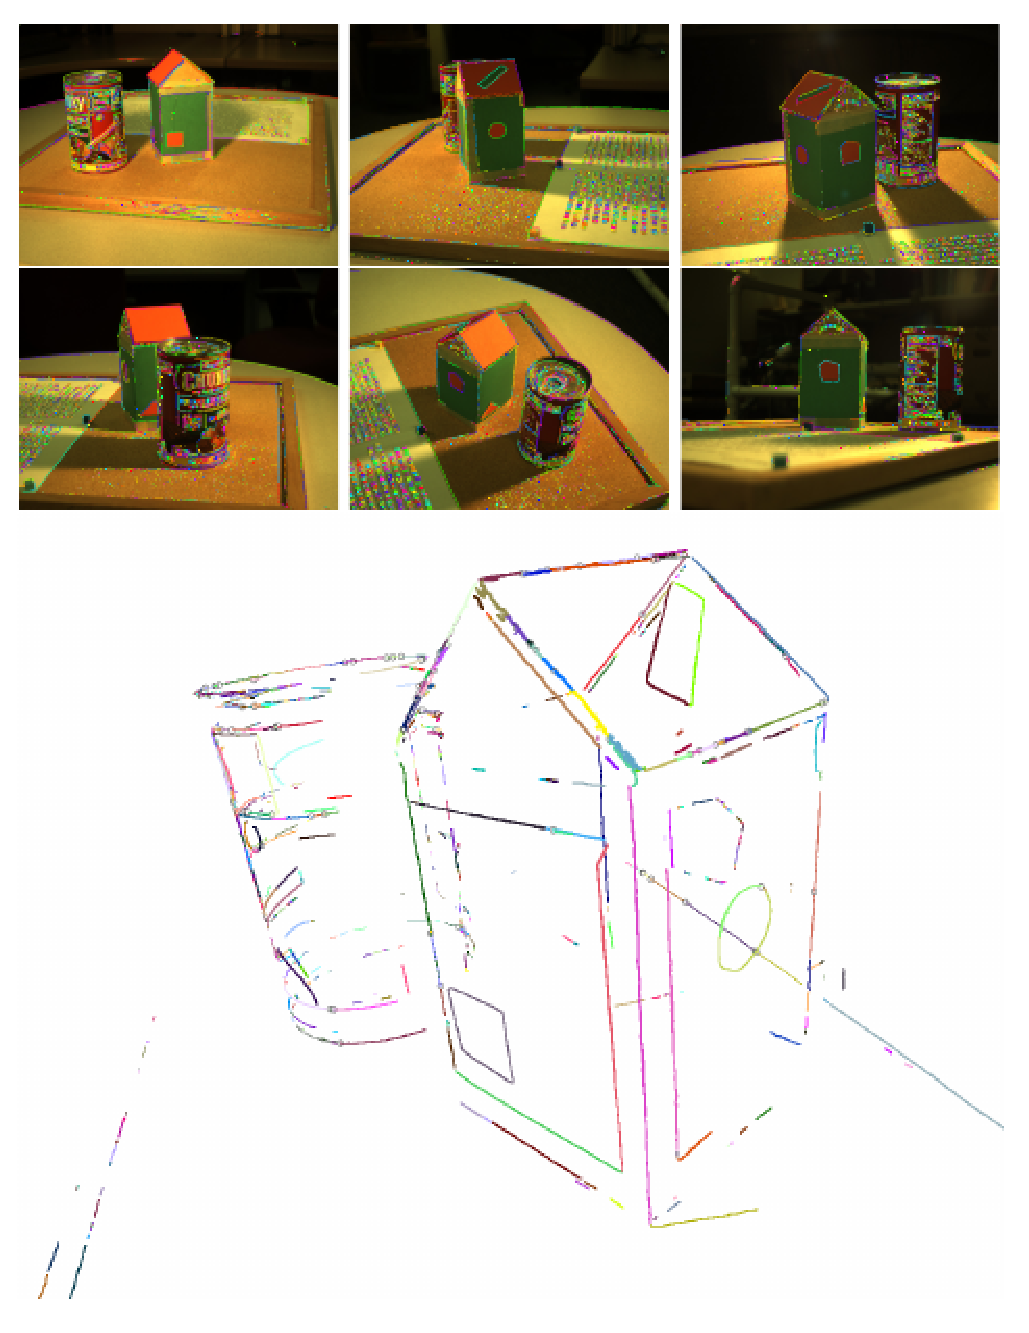
\includegraphics[scale=.7]{drawing2}
\caption{{\it A abordagem transforma um conjunto de imagens calibradas no desenho 3D, na forma de um gráfico consistindo de segmentos de curvas que se ligam nas junções.}}
\label{fig.drawing2}
\end{figure}

A maioria dos métodos de reconstrução não utilizam geometria diferencial de curvas, mas se baseiam em correlacionar pontos de interesse através das imagens e produzem uma desorganizada nuvem de pontos em 3D, figura \ref{fig.medusa}. Tais métodos obtêm sucesso em ambientes controlados, com cenas em larga escala e imagens ricas em textura, mas não podem ser aplicados em configurações gerais. Não podem reconstruir superfícies suaves e homogêneas nem suas fronteiras devido a esparsidade de pontos de interesse, como também não podem reconstruir regiões que se alteram drasticamente com a mudança de luz ambiente. Exemplos de imagens sujeitas a essas limitações são dados na figura \ref{fig.carro-objeto-curvo}.
\begin{figure}[!htb]
\centering
\subfloat{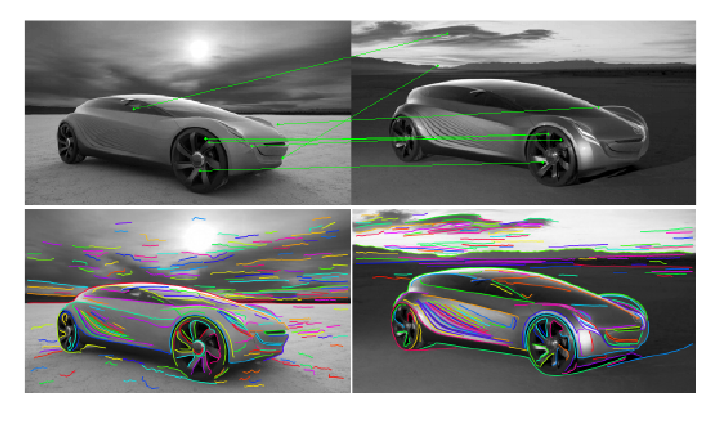
\includegraphics[scale=.76]{carro}}
\quad
\subfloat{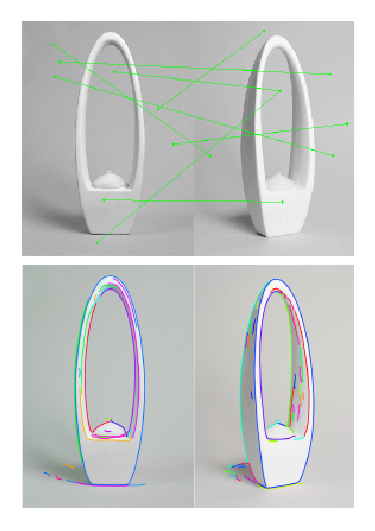
\includegraphics[scale=.6]{objeto-curvo}}
\caption{{\it Exemplos de objetos que não podem ser reconstruídos através da abordagem tradicional usando pontos de interesse e a geometria epipolar.}}
\label{fig.carro-objeto-curvo}
\end{figure}  
Daí são utilizadas outras técnicas de melhoramento dos resultados, como a interpolação de pontos e texturização, mas que não fornecem um resultado plenamente satisfatório. Podemos ver as fases desse processo em um exemplo no conjunto de imagens na figura \ref{fig.medusa}.

Portanto, ainda é necessário que se continuem as pesquisas em visão computacional, e o presente trabalho tem a finalidade de, primeiramente, detalhar as abordagens de artigos recentes na busca de novas combinações de ferramentas matemáticas que possam melhorar as atuais abordagens e atenuar o esforço computacional. Segundo, a verificação dos benefícios obtidos com o uso da geometria trifocal em transferência de pontos e reconstrução 3D em comparação com a geometria epipolar (mais usada atualmente), tudo com o objetivo de auxiliar na construção de uma nova abordagem usando geometria diferencial multifocal em condições realísticas.

\begin{figure}[!htb]
\centering
\subfloat{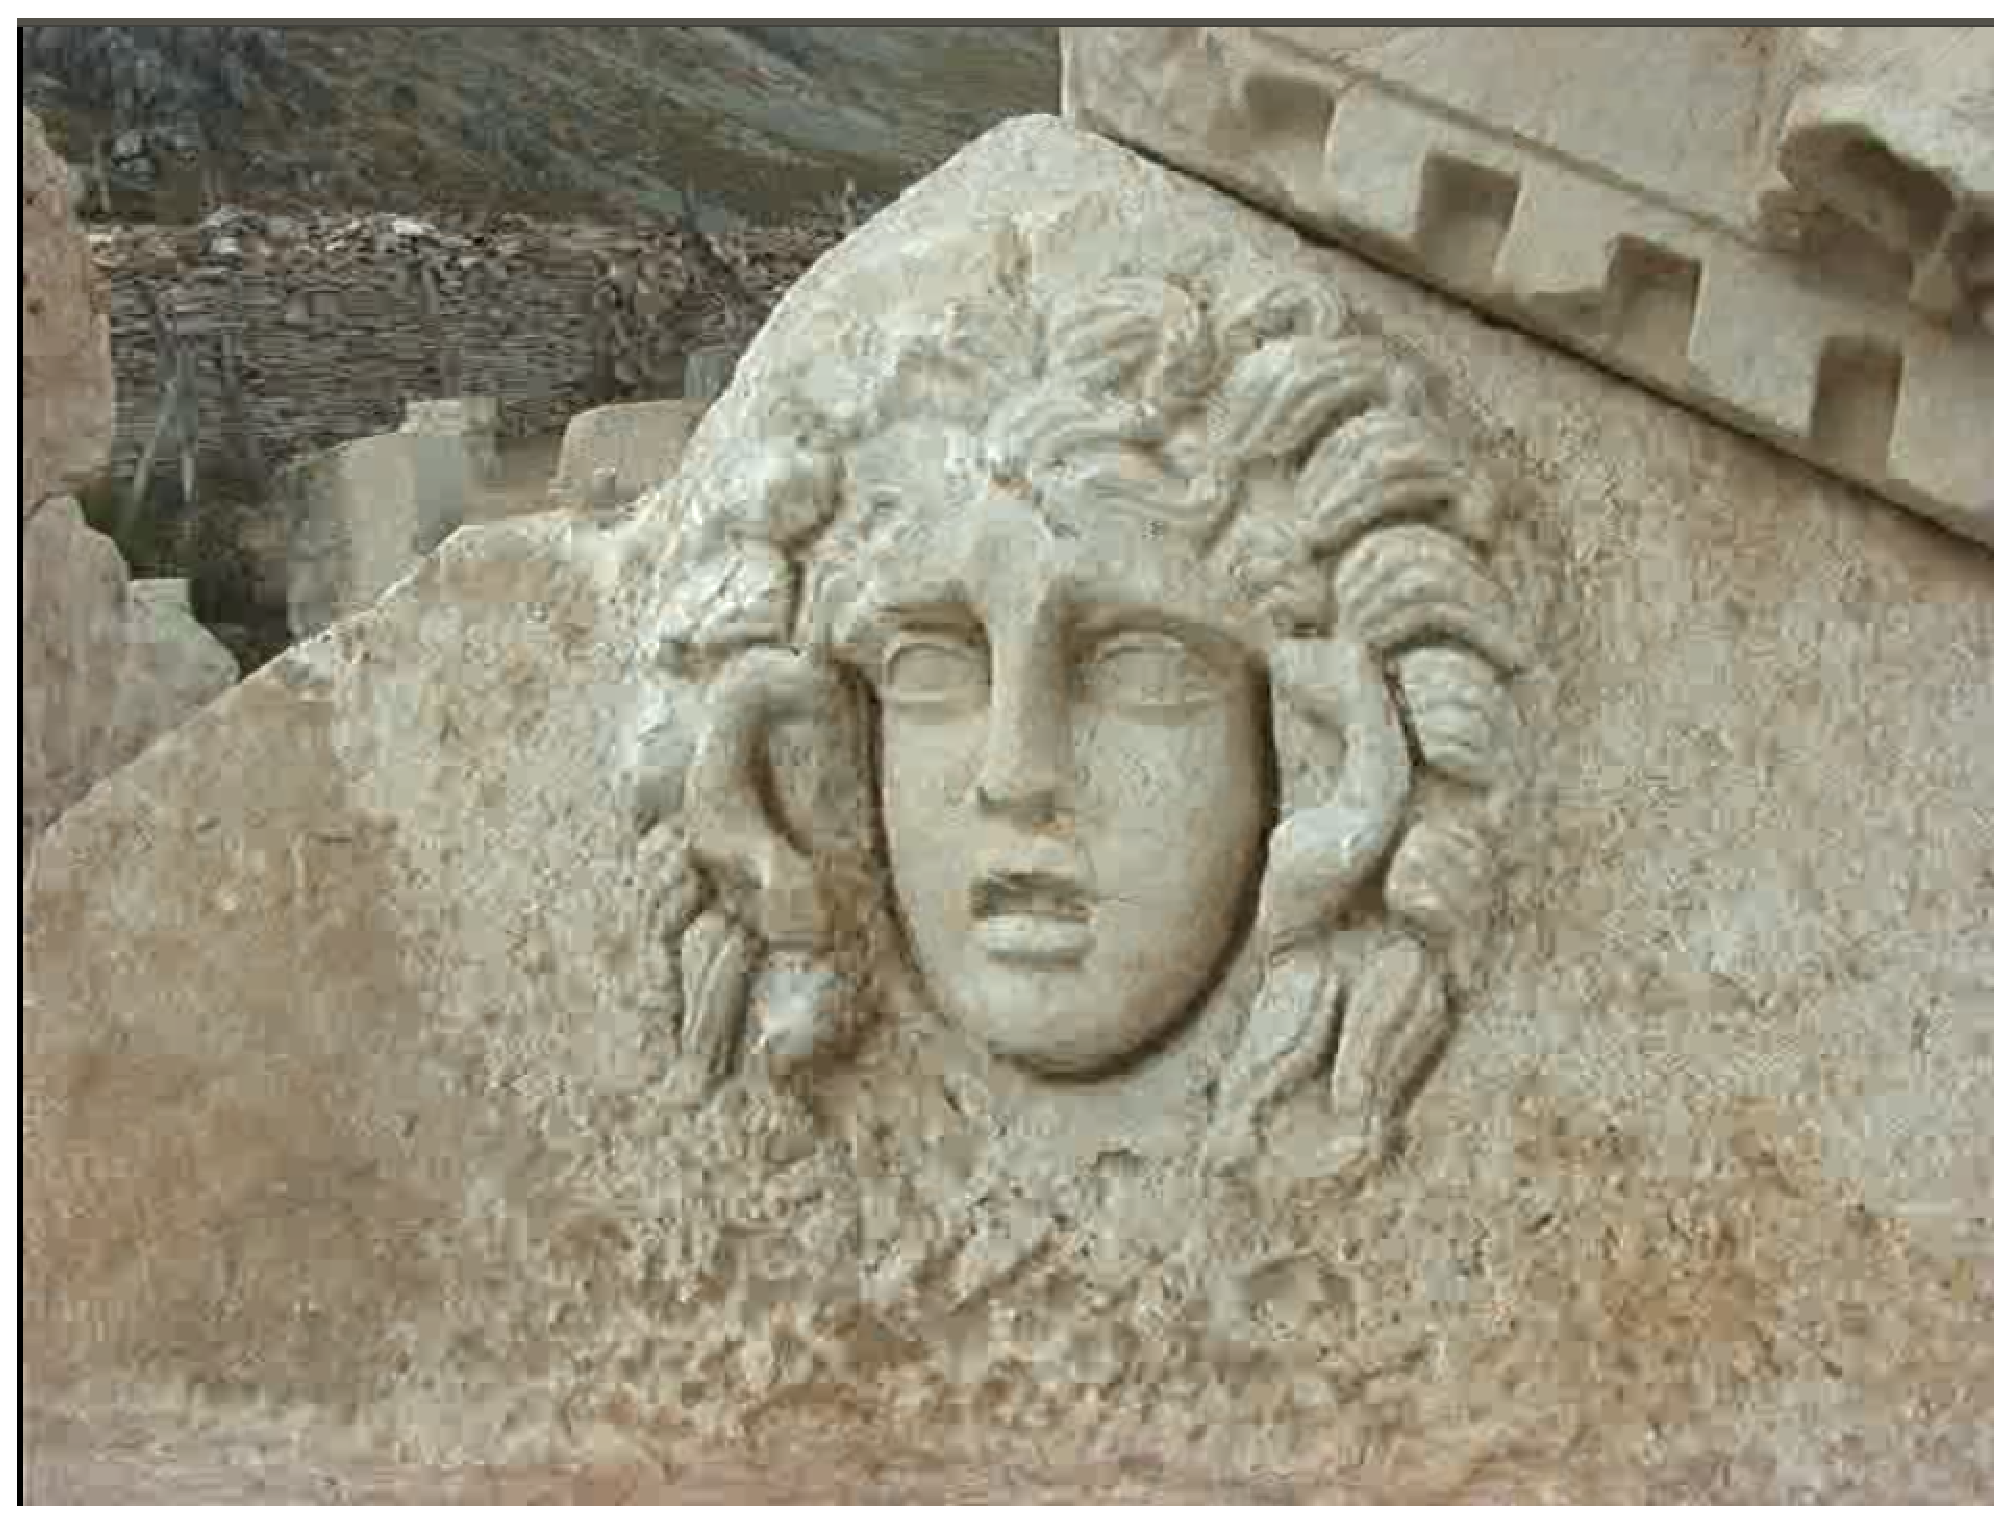
\includegraphics[scale=.2]{medusa1}}
\quad
\subfloat{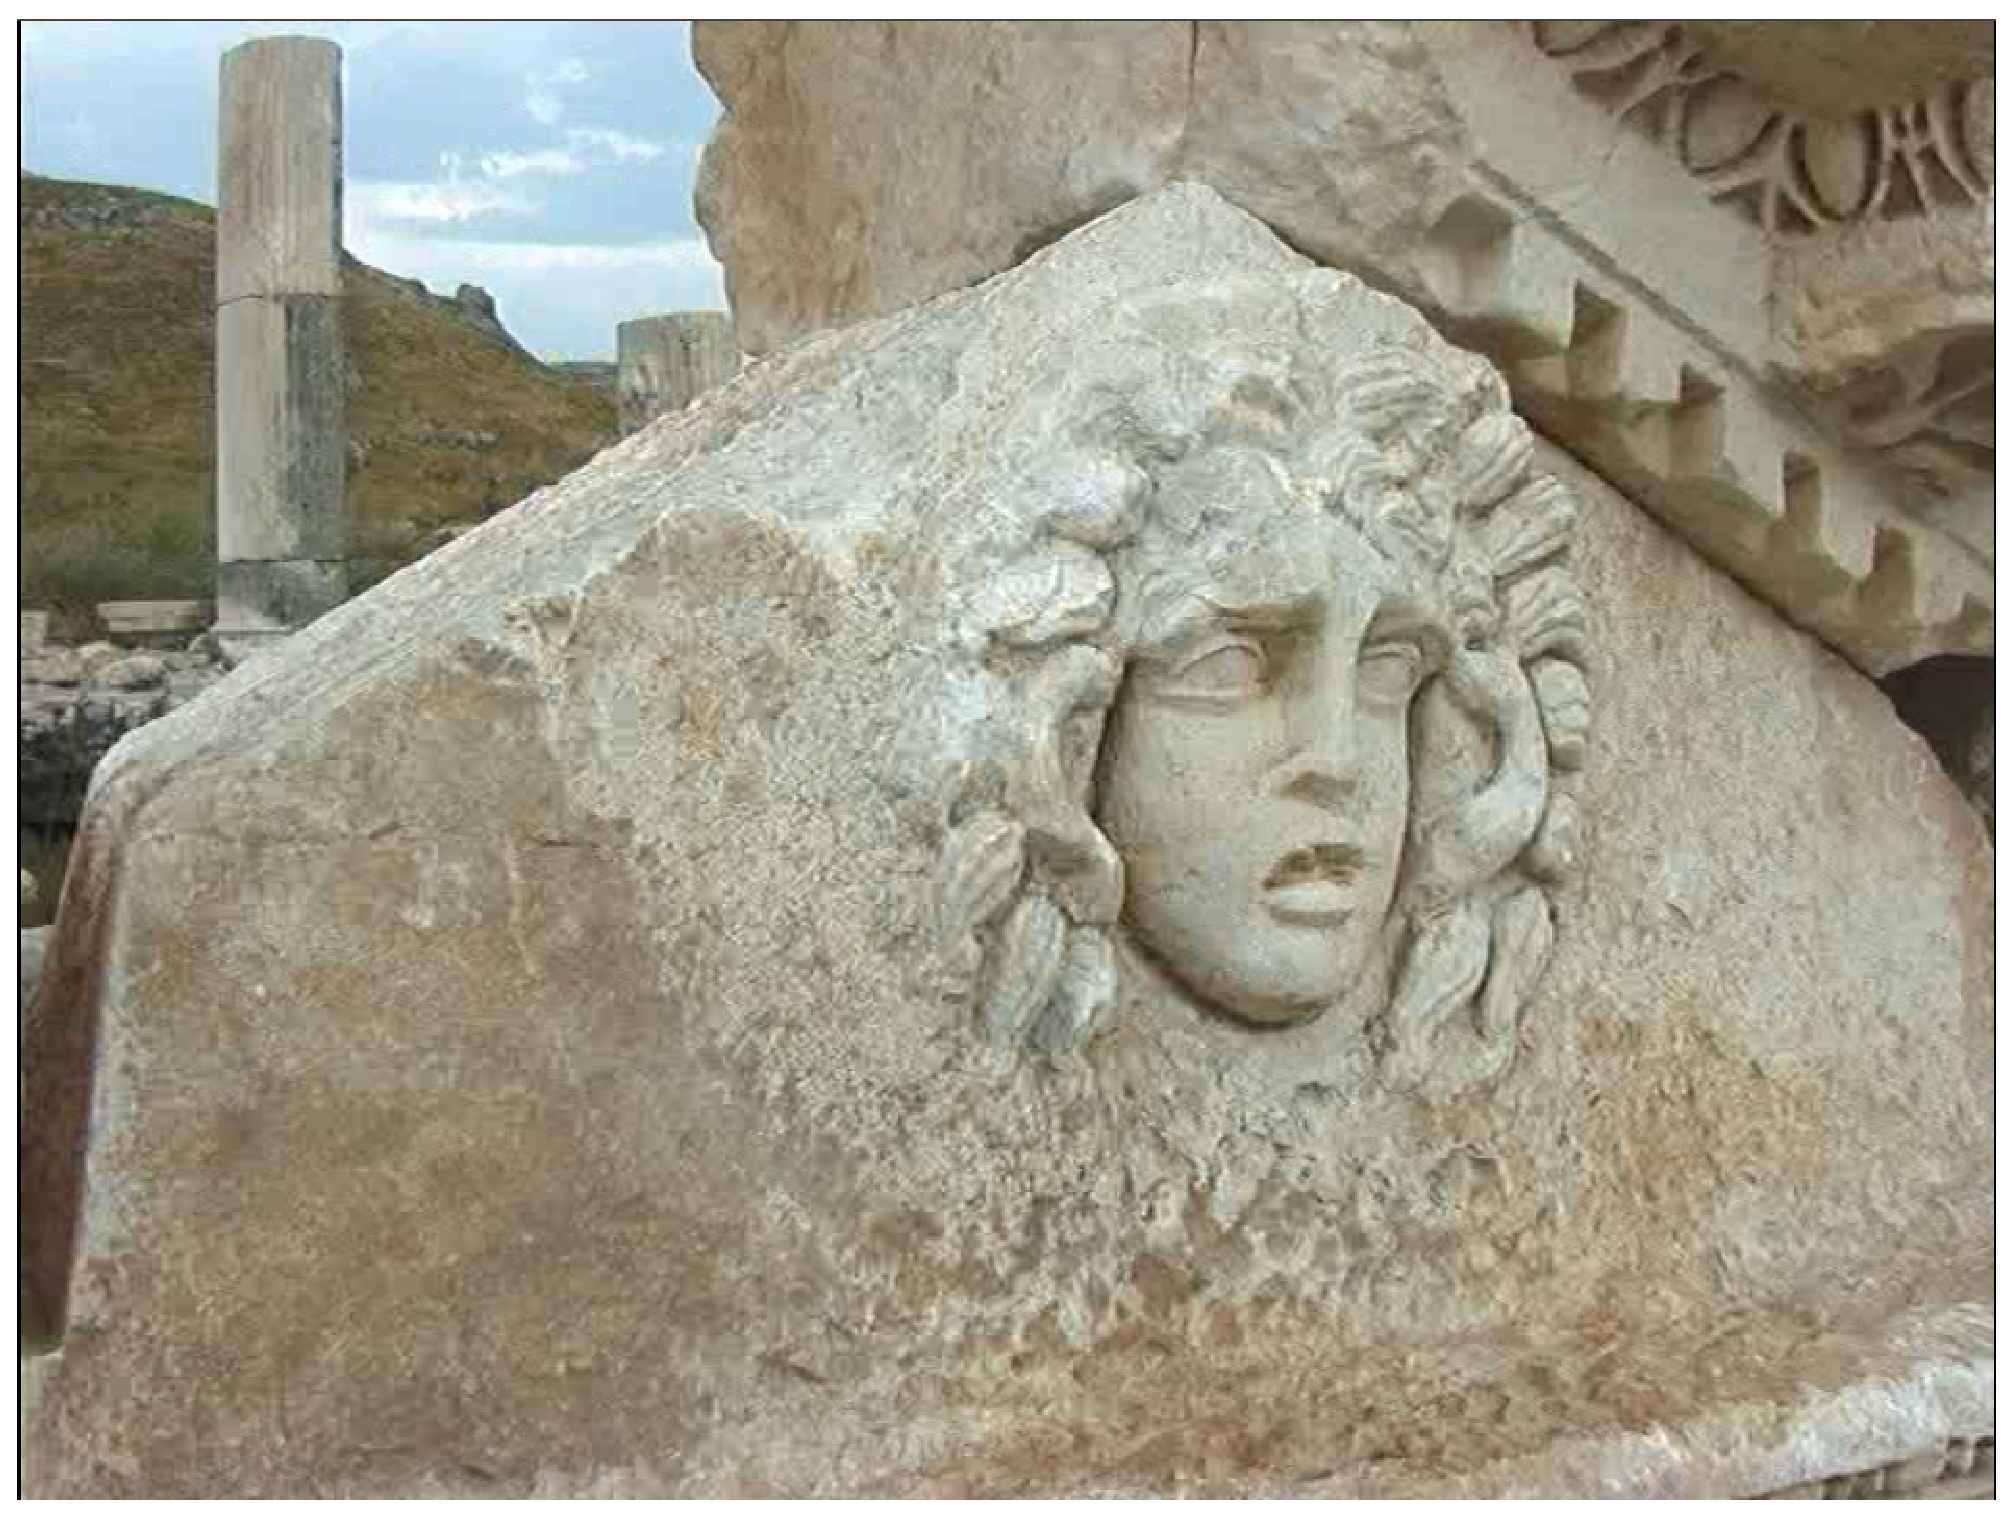
\includegraphics[scale=.2]{medusa2}}
\\
\subfloat{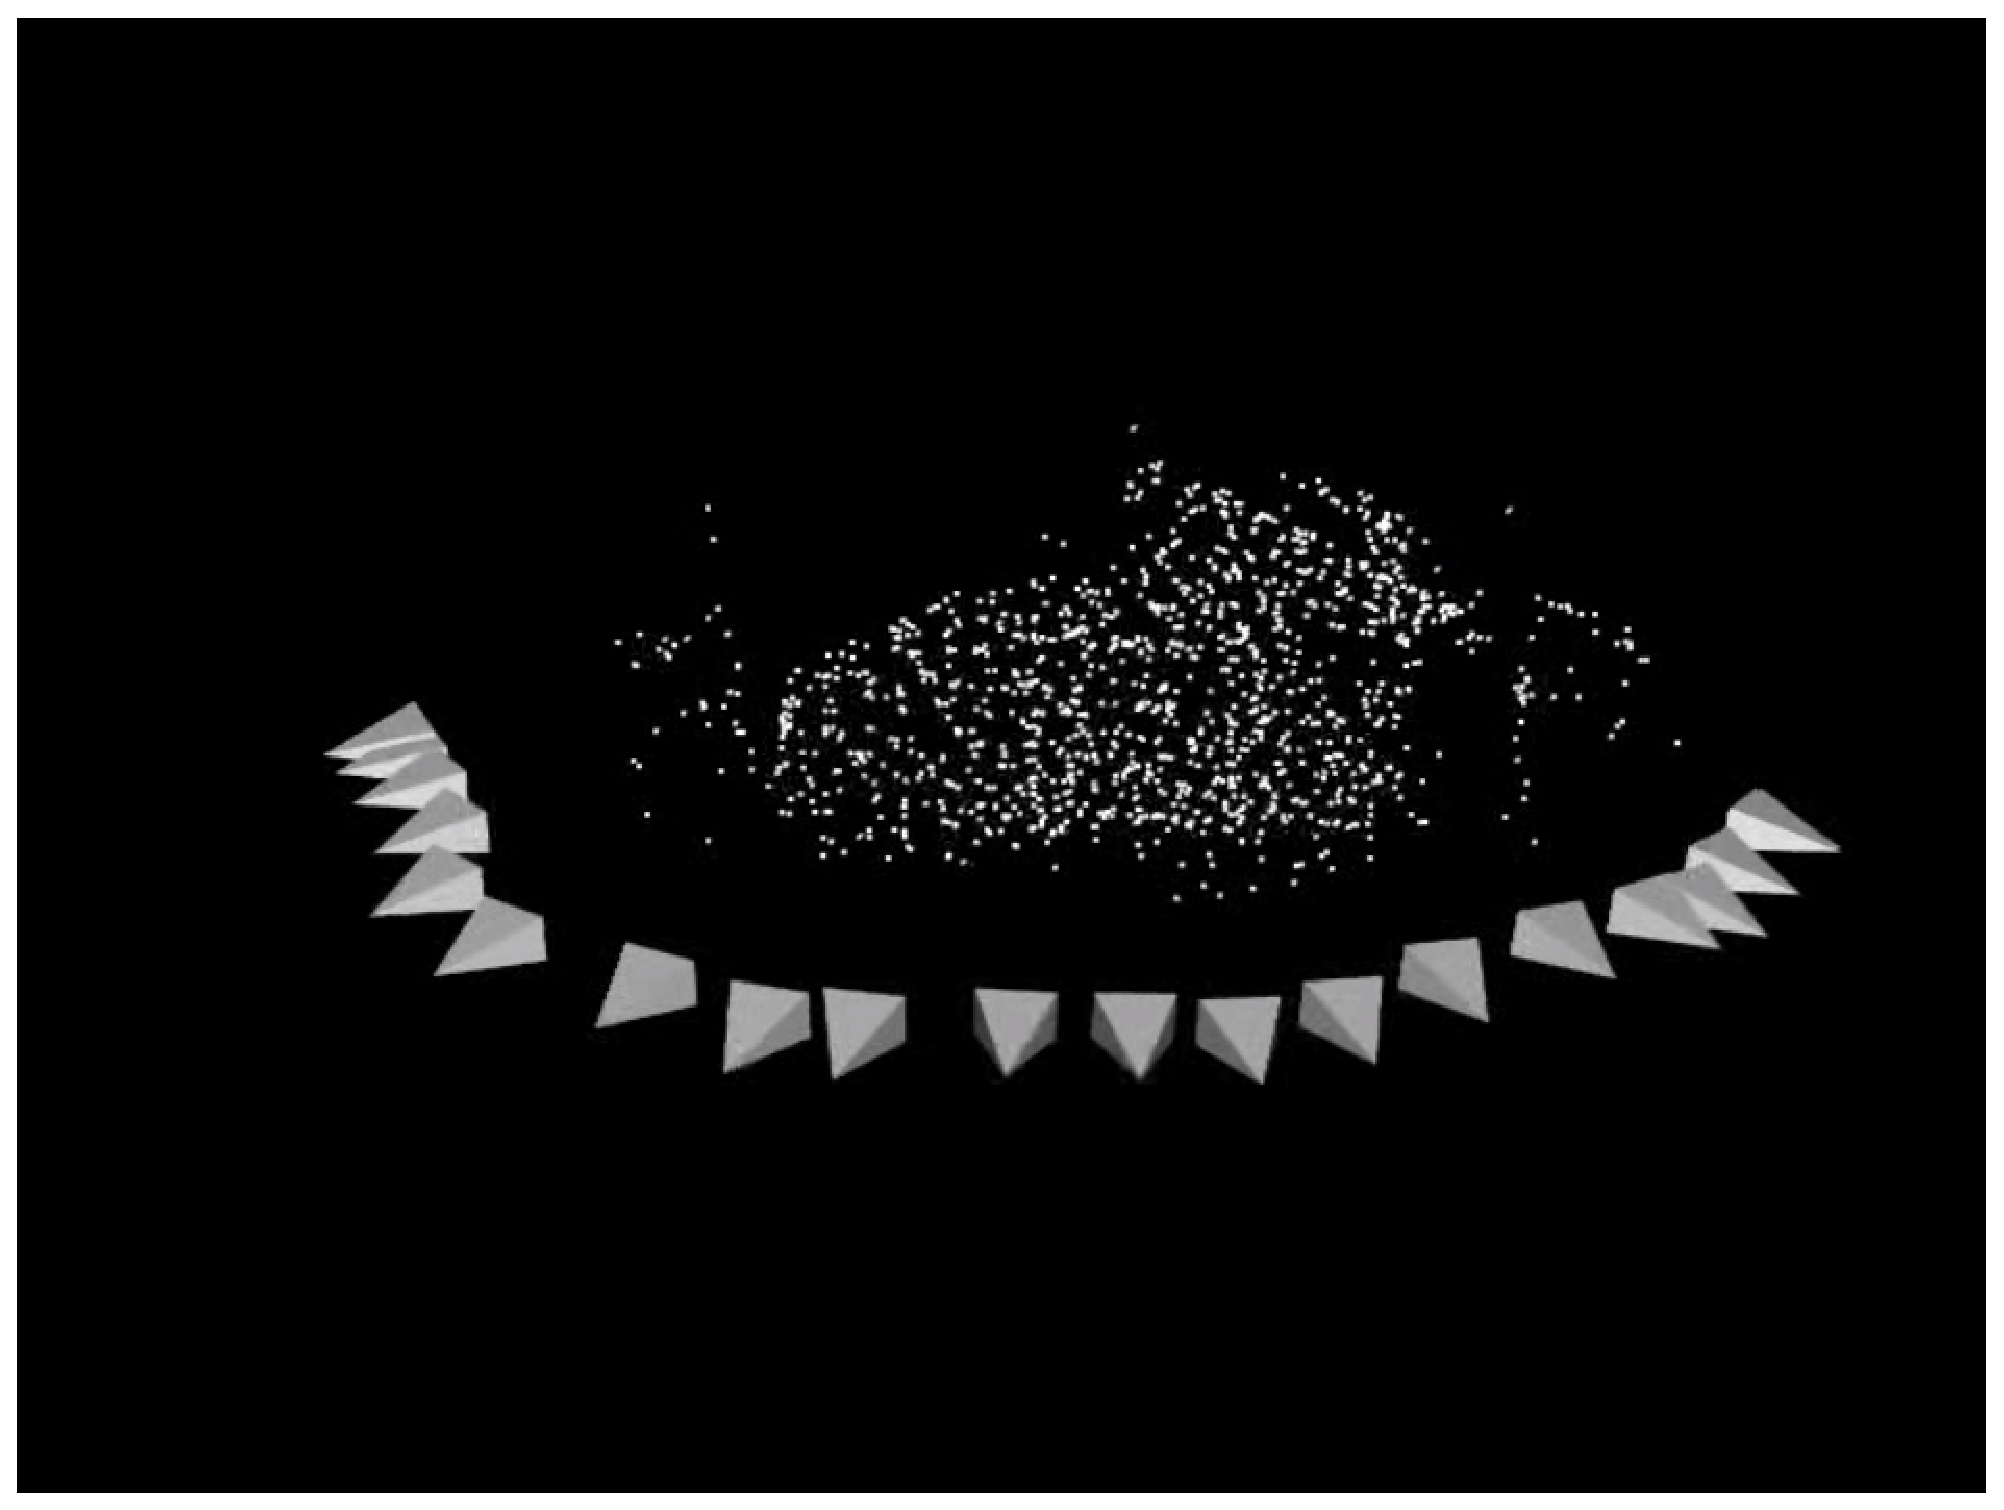
\includegraphics[scale=.2]{nuvem1}}
\quad
\subfloat{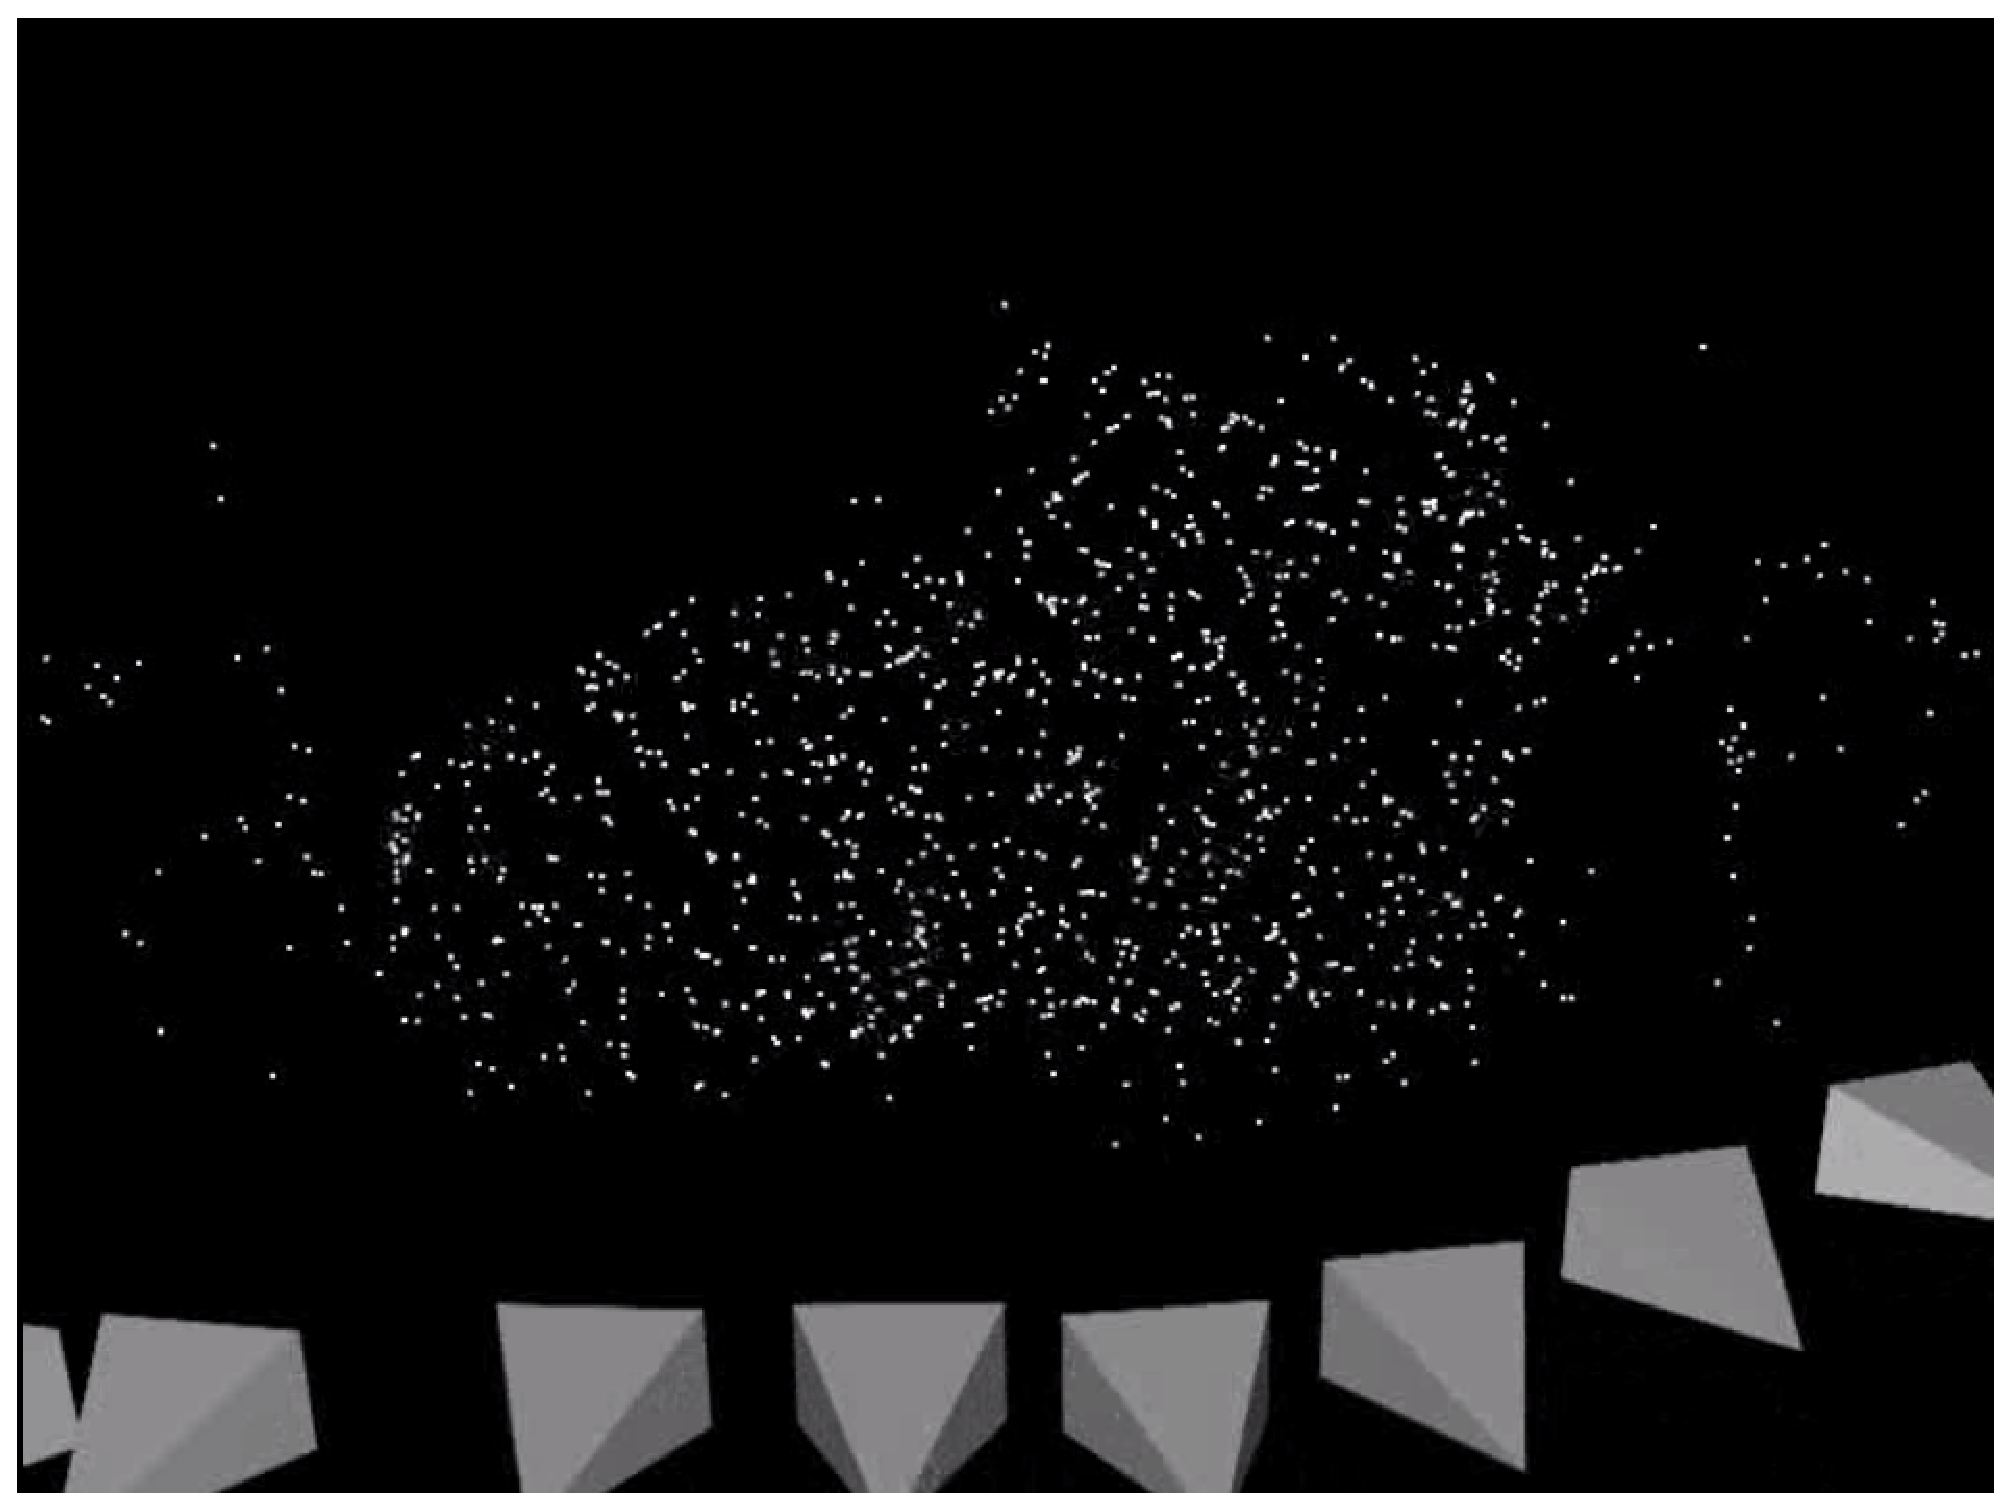
\includegraphics[scale=.2]{nuvem2}}
\\
\subfloat{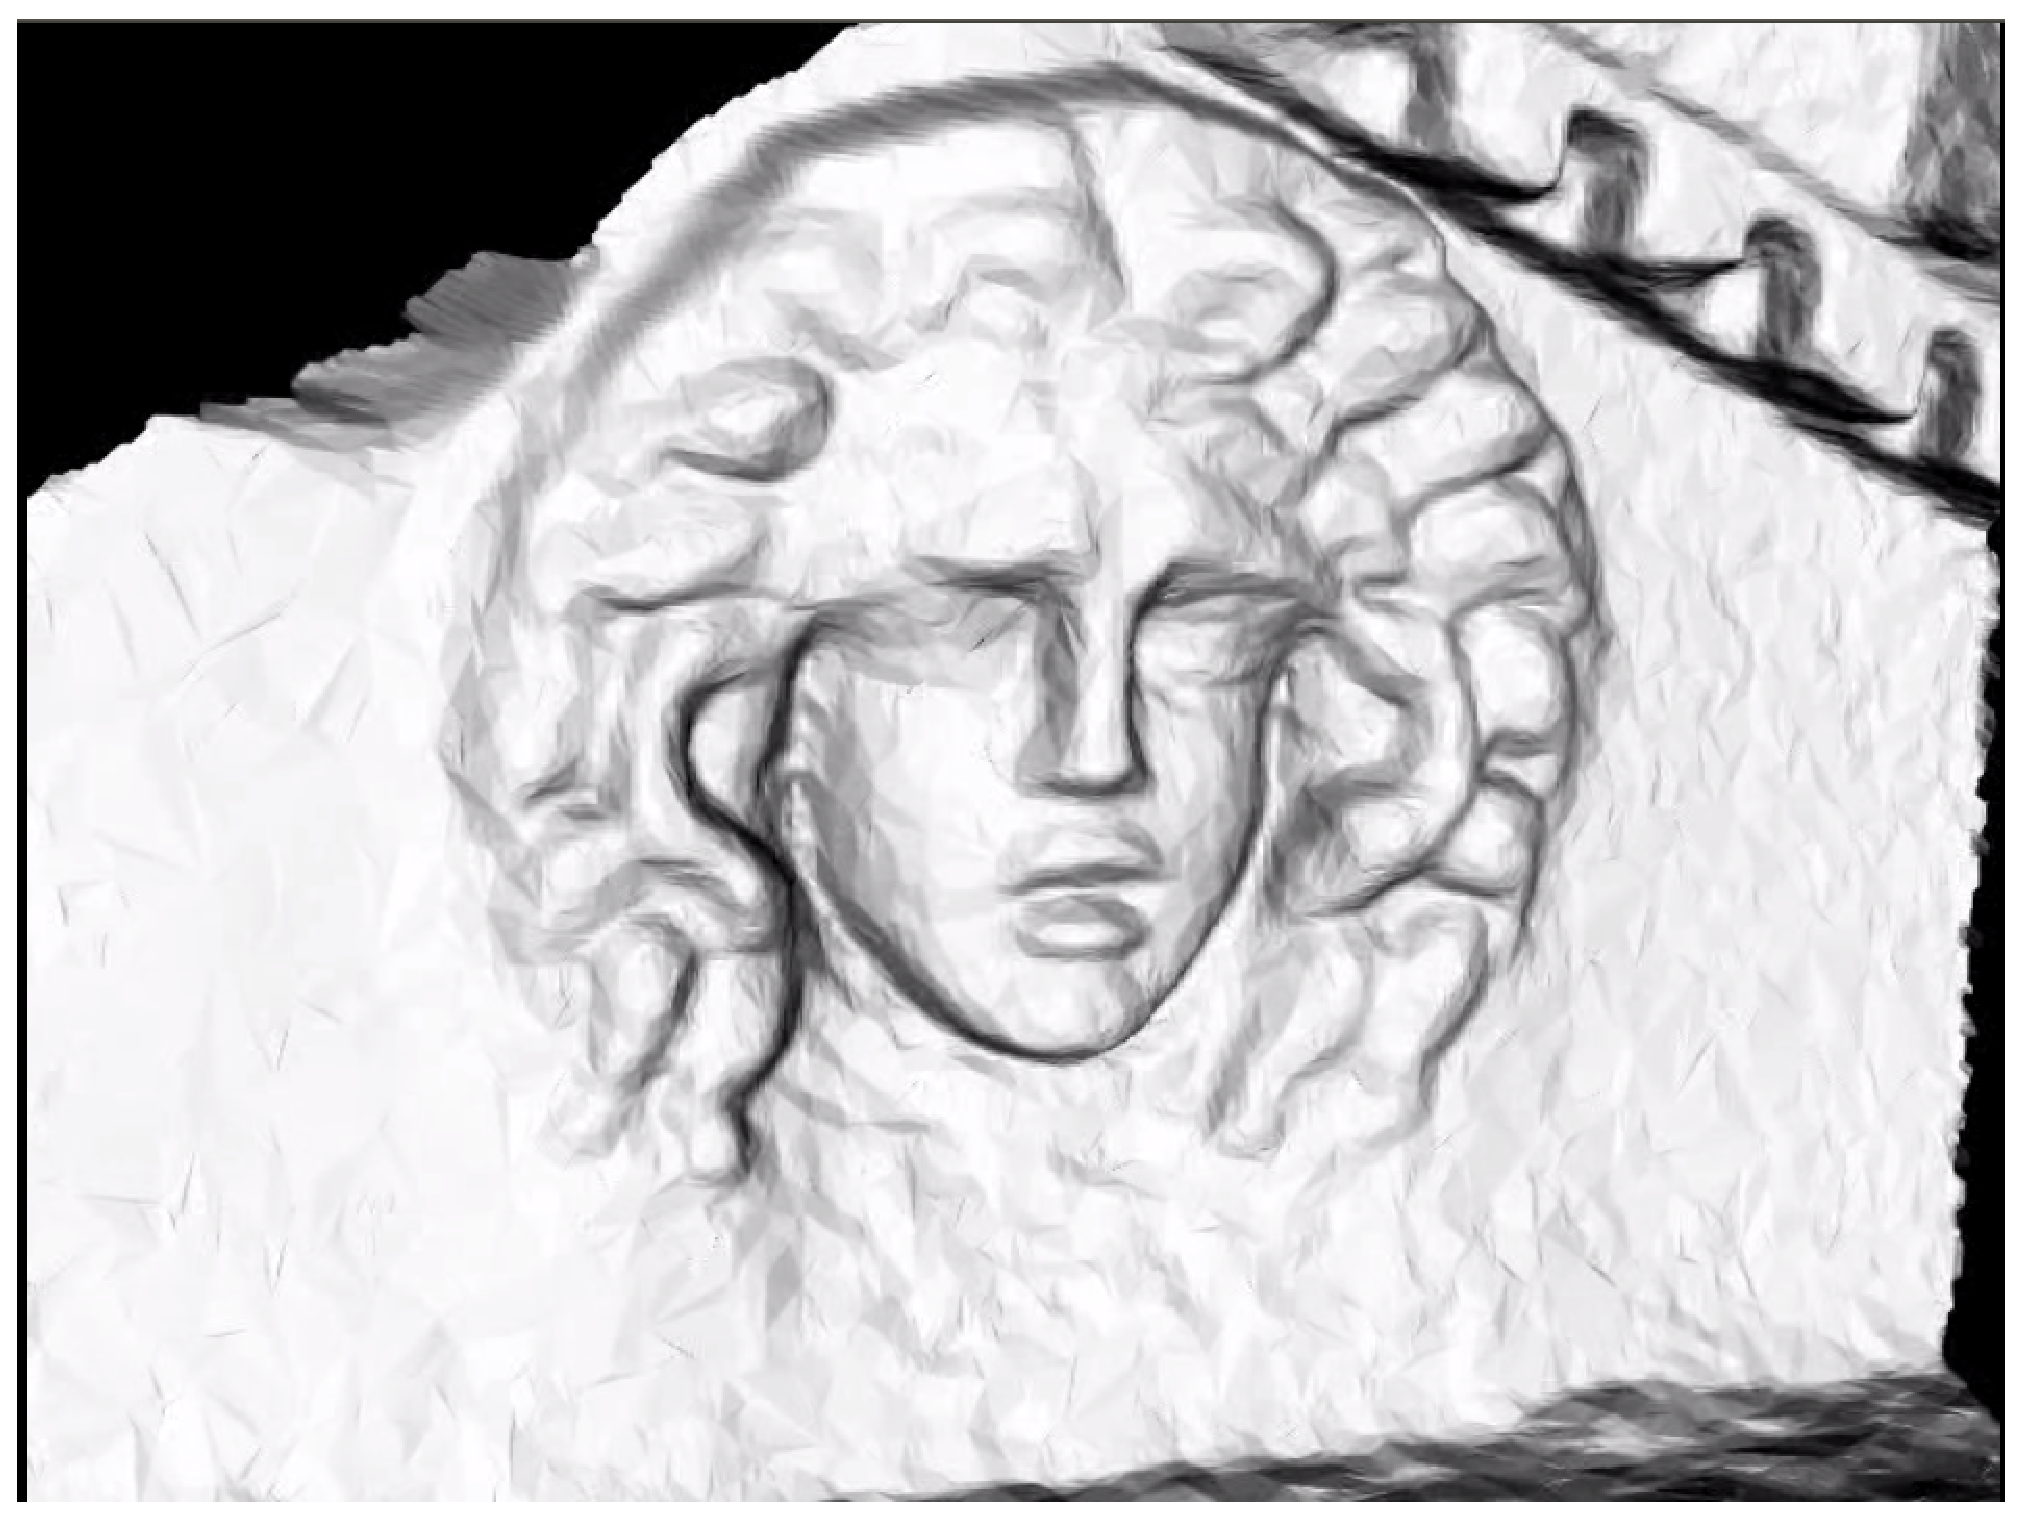
\includegraphics[scale=.2]{texturizacao2}}
\quad
\subfloat{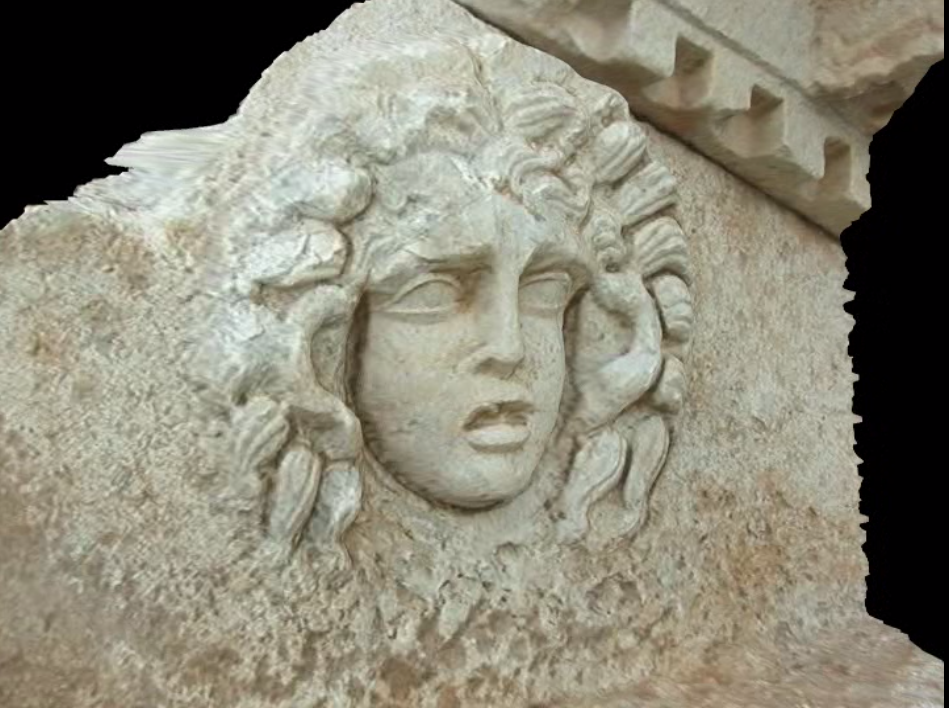
\includegraphics[scale=.2]{texturizacao-realmente}}
\caption{{\it Em cima, duas imagens extraídas de um vídeo (utilizado em reconstrução 3D) da estátua da Medusa em Sagalassos, Turquia. No meio, a nuvem de pontos obtida após a reconstrução 3D juntamente com as posições da câmera. Em baixo, aplicação de interpolação de pontos e texturização.}}
\label{fig.medusa}
\end{figure}

\subsection*{Visão geral e objetivos}

A seção \ref{sec.geo-1-2-cam} engloba a teoria básica de geometria projetiva utilizada em visão computacional 3D, com abordagens em termos de álgebra linear e usando o tipo de notação mais difundido entre pesquisadores da área. Além dos conceitos básicos, também são apresentados alguns conceitos e definições um pouco mais avançados indispensáveis ao entendimento das demais seções da dissertação, tudo com a finalidade de facilitar a compreensão do leitor sem a necessidade de consulta em outras publicações. Em seguida, há a apresentação da geometria epipolar, num sistema de visão estéreo com duas câmeras, bem como extração da matriz fundamental e a reconstrução das câmeras, usando essa abordagem bifocal que é mais comum do que a abordagem trifocal.

Na seção \ref{sec.astrom} temos o detalhamento de um artigo recente e representativo para a reconstrução de uma câmera a partir de objetos geométricos em 3D e suas respectivas imagens em 2D, \citep{bib:kuang}. A importância dessa publicação se verifica na utilização dos quatérnions de Hamilton para a parametrização da matriz de rotação da câmera, pois desta forma a matriz que possui nove componentes é parametrizada com apenas quatro variáveis. Outra vantagem é utilização das bases de Gr\"obner e da matriz de ação para solução computacional de sistemas de equações polinomiais de grau elevado e com muitas variáveis.

A geometria trifocal e suas características são abordadas na seção \ref{sec.geo-tri}, juntamente com a descrição dos benefícios do uso dessa geometria num sistema com três câmeras em comparação com uso da geometria epipolar entre cada par de câmeras. Após as comparações são apresentados métodos para a extração das matrizes fundamentais e métodos de reconstrução das câmeras a partir do tensor trifocal.  

Na seção \ref{sec.nister} há o detalhamento matemático da abordagem mais eficiente, até a presente data, para a reconstrução 3D das câmeras num sistema trifocal calibrado, \citep{2503343}. O artigo é bastante denso, com 25 teoremas, e apresenta a reconstrução de duas câmeras num sistema bifocal utilizando uma intrincada rede de conhecimentos de geometria projetiva. Depois da reconstrução das duas primeiras câmeras, é utilizada a reconstrução 3D de pontos para a reconstrução da terceira câmera, num procedimento similar ao apresentado na seção \ref{sec.astrom}, ou seja, os dois artigos quase se complementam. Esse trabalho deixa bem clara a dificuldade de se realizar a reconstrução num sistema com três imagens de quatro pontos 3D numa cena.

No apêndice \ref{sec.Apen-A} são fornecidas ferramentas de álgebra linear acompanhadas de algumas definições mais restritas à assimilação da dissertação. No apêndice \ref{sec.geo-algebrica} há uma breve introdução aos conceitos básicos de geometria algébrica seguidos da apresentação (informal e em termos de exemplos) de uma teoria para resolução de sistemas de equações polinomiais com várias variáveis.


\section{Geometria de Uma e Duas Câmeras}
Nesta seção, faremos uma breve introdução aos conceitos básicos de Geometria Projetiva e usaremos a notação contida em \cite{Hartley2004}, por ser o tipo de notação mais difundido entre pesquisas de visão computacional. Para uma abordagem mais profunda do assunto o leitor pode pesquisar o referido autor.  

\subsection{O Espaço Projetivo em Duas Dimensões}\label{sec.espaco-P2}


\subsubsection{A Reta.}\label{sec.reta}


Sabemos que uma reta no plano $\mathbb{R}^{2}$ pode ser representada pela equação $a\,x+b\,y+c=0$, onde a reta fica perfeitamente determinada pelos valores das constantes $a,b,c$. Desta forma, podemos representar retas através de vetores, e assim a reta $a\,x+b\,y+c=0$ seria representada por $(a,b,c)^\top \in \mathbb{R}^{3}$, utlizando o símbolo em negrito $\lightrgb$ para indicar tal vetor escrito em coluna, por padrão. Portanto $\lightrgb = (a,b,c)^\top$. Note que a relação entre uma dada reta e o seu respectivo vetor não é biunívoca, pois o vetor $k\,(a,b,c)^\top$, tal que $k \in \mathbb{R}$, representa a reta $k\,a\,x+k\,b\,y+k\,c=0$ que é a mesma reta $a\,x+b\,y+c=0$. Temos, então, infinitos vetores (chamados paralelos na Álgebra Linear) que representam uma mesma reta e formam uma classe de equivalência, onde essa classe pode ser representada por qualquer um de seus vetores. Os vetores de uma classe de equivalência, definida pela multiplicação por um escalar, são conhecidos como vetores {\it homogêneos}. O conjunto de classes de equivalência de vetores em $\mathbb{R}^{3} - (0,0,0)^\top$ forma o {\it Espaço Projetivo} $\mathbb{P}^{2}$. O vetor $(0,0,0)^\top$ foi excluído por não representar reta alguma. Após essas considerações, dizemos que uma reta no plano é representada pelo vetor $(a,b,c)^\top$ em {\it coordenadas homogêneas}. Já que para determinar uma reta precisamos determinar os valores do três parâmetros $a,b \,\,\text{e}\,\, c$, vemos que uma reta tem três graus de liberdade.\\

\subsubsection{O Ponto.}\label{sec.ponto}


Sabemos que em $\mathbb{R}^{2}$ os pontos são representados através de pares ordenados do tipo $(x,y)$, e assim cada ponto pode ser identificado como um vetor $(x,y)^\top$. Os vetores que se referem a pontos serão representados pelo símbolo em negrito $\x$, que sempre indicará um vetor coluna. Desse jeito, $\x=(x,y)^\top$. Sabemos também que um ponto $(x,y)^\top$ pertence a uma reta $(a,b,c)^\top$ se, e somente se, $a\,x+b\,y+c=0$, e podemos realizar essa verificação utilizando multiplicação matricial, escrevendo $\x$ com uma terceira coordenada igual a 1:

\begin{equation*}
(x,y,1)^\top 
\begin{pmatrix}
 a  \\ 
 b  \\ 
 c 
 \end{pmatrix} 
 = 0 \qquad 
 \text{ou} 
 \qquad \x ^\top\lightrgb = 0.
\end{equation*}

Ou seja, temos um ponto de $\mathbb{R}^{2}$ representado como um vetor com três coordenadas. Observe que para $k \in \mathbb{R} - \{0\}$, temos:

\begin{equation*}
(k\,x,k\,y,k)^\top 
\begin{pmatrix}
 a  \\ 
 b  \\ 
 c 
 \end{pmatrix} 
 = 0
 \qquad \Leftrightarrow \qquad
 (x,y,1)^\top
\begin{pmatrix}
 a  \\ 
 b  \\ 
 c 
 \end{pmatrix} 
 = 0.
\end{equation*}

Portanto,  variando $k$, podemos considerar os vetores em coordenadas homogeneas $(k\,x,k\,y,k)^\top \in \mathbb{P}^2$, como representantes do mesmo ponto $(x,y)^\top \in \mathbb{R}^2$, e podemos resgatar nossa representaçao original aplicando o procedimento $(x/k,y/k)^\top$, pois $k \ne 0$.

\begin{figure}[!htb]
\centering
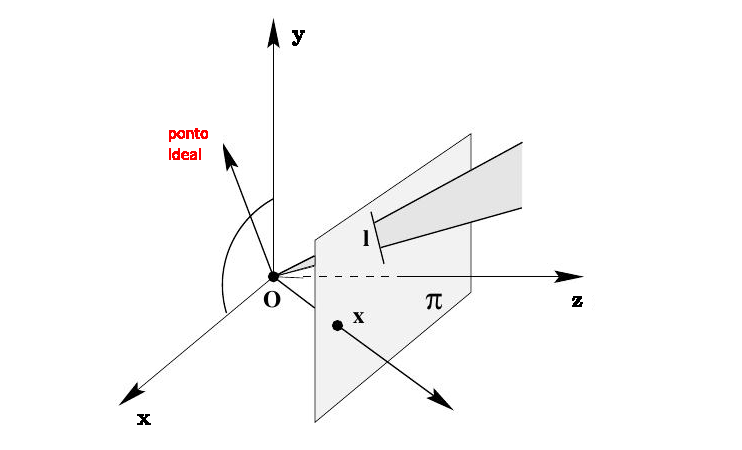
\includegraphics[scale=1]{espaco_P2}
\caption{\textit{O plano $\bpi$ representa o espaço projetivo $\mathbb{P}^2$. Pontos e retas pertencentes a esse espaço são representados, respectivamente, por vetores e planos que passam pela origem do $\mathbb{R}^3$. O ponto ideal é representado por um vetor que pertence ao plano $x\,y$, o qual é paralelo ao plano $\bpi$. O plano $x\,y$ representa a reta no infinito.}}
\label{plano_P2}
\end{figure}

Podemos pensar no espaço projetivo como um conjunto de raios passando pela origem do $\mathbb{R}^3$, onde cada raio representa um único ponto, que é a interseção desse raio com o plano $\mathbb{P}^2$. Desta mesma forma, retas em $\mathbb{P}^2$ são formadas por planos. Na figura \ref{plano_P2}, podemos observar como a interseção do raio com o plano define um ponto, assim como a interseção de dois planos definem uma reta.


Para determinar um ponto precisamos determinar os valores das duas primeiras coordenadas do vetor homogêneo que representa esse ponto, já que a terceira coordenada está em função das duas primeiras. Assim, dizemos que um ponto tem dois graus de liberdade e a terceira coordenada pode ser usada para fixar uma escala.
\\

\subsubsection{Retas determinadas por dois pontos e a interseção de duas retas.}

A representação de retas em coordenadas homogêneas nos permite calcular a interseção de duas retas usando o produto vetorial. Sabemos que o produto vetorial de dois vetores, digamos $\lightrgb\times\lightrgb'$ em $R^3$ resulta num terceiro vetor que é ortogonal ao plano definido pelos vetores $\lightrgb$ e $\lightrgb'$. Em particular, esse terceiro vetor $\lightrgb\times\lightrgb'$ será ortogonal a qualquer dos vetores $\lightrgb$ e $\lightrgb'$, assim seu produto escalar é zero:

\begin{equation*}
\lightrgb\cdot(\lightrgb\times\lightrgb')=\lightrgb'\cdot(\lightrgb\times\lightrgb')=0.
\end{equation*}
O produto escalar também pode ser representado por multiplicação matricial, assim

\begin{equation}\label{eq.pro-vet}
\lightrgb^\top(\lightrgb\times\lightrgb')=\lightrgb'^\top(\lightrgb\times\lightrgb')=0,
\end{equation}
mas sendo $\x$ o ponto de interseção entre as duas retas temos que

\begin{equation}\label{eq.pro-vet-2}
\lightrgb^\top\x=\lightrgb'^\top\x=0
\end{equation}
o que, comparando \ref{eq.pro-vet} e \ref{eq.pro-vet-2}, nos sugere que

\begin{equation*}
\x=\lightrgb\times\lightrgb'.
\end{equation*}


Com argumento análogo podemos constatar que dois pontos definem uma reta através do produto vetorial entre eles, pois basta verificar que dois pontos $\x$ e $\x'$ pertencem a reta definida por

\begin{equation*}
\lightrgb=\x\times\x'.
\end{equation*}\\


\noindent {\bf Pontos Ideais e a Reta no Infinito.}

Duas retas paralelas no espaço Euclidiano tem equações

\begin{equation*}
a\,x+b\,y+c=0\qquad\text{e}\qquad a\,x+b\,y+c'=0
\end{equation*}
com coordenadas homogêneas

\begin{equation*}
\lightrgb=(a,b,c)^\top\qquad\text{e}\qquad\lightrgb'=(a,b,c')^\top.
\end{equation*}
Computando a interseção entre as duas retas e ignorando o fator de escala $(c'-c)$ temos

\begin{equation*}
\begin{array}{rcl}
\lightrgb\times\lightrgb'&=&(a,b,c)^\top\times(a,b,c')^\top\\
&=&(c'-c)\,(b,-a,0)^\top\\
&=&(b,-a,0)^\top,
\end{array}
\end{equation*}
e se tentarmos encontrar as coordenadas não homogêneas do ponto de interseção temos

\begin{equation*}
\left(\frac{b}{0},\frac{-a}{0}\right)^\top,
\end{equation*}
o que não faz sentido matematicamente mas sugere que o ponto tem coordenadas que tendem ao infinito. Vetores homogêneos $(x,y,z)^\top$ com $z\neq0$ correspondem a pontos finitos em $R^2$ e, se $z=0$, os pontos são conhecidos como \textit{pontos ideais} ou \textit{pontos no infinito} em geometria projetiva.

Se tomarmos um ponto no infinito genericamente $\x=(x,y,0)^\top$ percebemos que ele pertence a uma determinada reta $\lightrgb_\infty=(0,0,1)^\top$, pois

\begin{equation*}
\lightrgb_\infty^\top \x=(0,0,1)
\begin{pmatrix}
x\\
y\\
0
\end{pmatrix}
=0,
\end{equation*} 
e tal reta é conhecida como \textit{reta no infinto}. Assim, no plano projetivo temos que retas paralelas se encontram em ponto no infinito e o conjunto de pontos no infinito constituem a reta no infinito.

Um fato interessante sobre pontos no infinito é que eles constituem as direções das retas no plano projetivo $\mathbb{P}^2$. Observe que a interseção de uma reta qualquer $\lightrgb=(a,b,c)^\top$ com a reta no infinito $\lightrgb_\infty=(0,0,1)^\top$,

\begin{equation*}
[\lightrgb]_\times \lightrgb_\infty=(b,-a,0),
\end{equation*}
é um vetor que, em coordenadas não homogêneas $(b,-a)$, é ortogonal ao vetor $(a,b)$, que é o vetor normal à reta dada $\lightrgb=(a,b,c)^\top$. Assim $(b,-a)$ constitui-se a direção da reta $\lightrgb$, e como a reta no infinito contém todos os pontos do tipo $(b,-a)$, dizemos que a reta no infinito é o conjunto de direções das retas no plano projetivo $\mathbb{P}^2$.\\





\subsubsection{A Cônica.}


Em geometria Euclidiana, as cônicas são de três tipos principais: elipse, hipérbole e parábola. São definidas, algebricamente, por uma equação do segundo grau em duas variáveis, considerando coordenadas não homogêneas:

\begin{equation*}
a\,x^2+b\,x\,y+c\,y^2+d\,x+e\,y+f=0.
\end{equation*}

Sabemos que um ponto pertence à cônica se ele é solução da equação acima, a qual pode ser representada utilizando multiplicação matricial e vetores em coordenadas homogêneas, com a terceira coordenada configurada como 1:

\begin{equation*}
(x,y,1)^\top 
 \begin{bmatrix}
a & b/2 & d/2\\
b/2 & c & e/2\\
d/2 & e/2 & f
\end{bmatrix}
 \begin{pmatrix}
x\\
y\\
1
\end{pmatrix}
 = 0.
\end{equation*}

Podemos generalizar essas coordenadas homogêneas fazendo as substituições $x = x_{1}/x_{3}$ e $y = x_{2}/x_{3}$, e nossa equação do elípse fica:

\begin{equation*}
a\,x_1^2+b\,x_1\,x_2+c\,x_2^2+d\,x_1\,x_3+e\,x_2\,x_3+f\,x_3^2=0.
\end{equation*}

Novamente em notação matricial:

\begin{equation*}
(x_1,x_2,x_3)^\top 
 \begin{bmatrix}
  a & b/2 & d/2\\
  b/2 & c & e/2\\
  d/2 & e/2 & f
  \end{bmatrix}
 \begin{pmatrix}
  x_1\\
  x_2\\
  x_3
  \end{pmatrix}
 = 0
 \qquad \text{ou} \qquad
 \x^\top C\,\x = 0.
\end{equation*}

Já que um ponto pertence à cônica se, e somente se, satisfaz a última equação, temos que $C$ fica definida como a matriz que representa uma cônica no espaço projetivo $\mathbb{P}^2$.

\begin{equation*}
C =  \begin{bmatrix}
      a & b/2 & d/2\\
      b/2 & c & e/2\\
      d/2 & e/2 & f
      \end{bmatrix}.
\end{equation*}

Percebemos que as cônicas são representadas por matrizes $3\times3$ simétricas e, portanto, possuem seis variáveis. Usando uma dessas variáveis para fixar a escala, temos que as cônicas possuem cinco graus de liberdade. Podemos, por exemplo, dividir todas as coordenadas da matriz $C$ por $f$. \\

\subsubsection{Retas tangentes à cônicas.} 

Uma reta tangente a uma cônica num ponto $\x$ qualquer tem a simples forma

\begin{equation*}
\lightrgb=C\x.
\end{equation*}
De fato, se a reta $\lightrgb$ passa por um ponto $\x$ temos que $\x^\top\lightrgb=0$, e se esse ponto $\x$ pertence à cônica $C$ então $\x^\top C\,\x=0$. Se $\x$ é o único ponto de interseção da reta com a cônica, comparando as duas relações  temos que $\lightrgb=C\x$ é a tangente procurada. Se a reta passa também por um outro ponto $\y$ na cônica, temos que $\y^\top C\,\y=0$ e $\lightrgb^\top\y=0$. Mas como $\lightrgb=C\x$ e considerando que $C$ é simétrica, temos

\begin{equation*}
\lightrgb^\top\y=(C\x)^\top\y=\x^\top C\,\y=0.
\end{equation*}  
Agora considerando todos os pontos em $\lightrgb=(\x+\alpha\y)$ parametrizados por $\alpha$, vamos verificar que todos eles pertencem à cônica $C$ usando as relações anteriores:

\begin{equation*}
(\x+\alpha\y)^\top C\,(\x+\alpha\y)=\x^\top C\,\x+\alpha\y^\top C\,\x+\x^\top C\,\alpha\y+\alpha\y^\top C\,\alpha\y=0,
\end{equation*}
já que cada uma das parcelas é zero. Assim toda a reta $\lightrgb$ ligando $\x$ e $\y$ está em $C$, que neste caso é dita ser uma cônica degenerada.\\

\subsubsection{Cônica Dual ou de reta.} 

A cônica definida por $\x^\top C\,\x=0$ é chamada cônica ponto já que é definida por uma equação que envolve pontos. Mas como pontos e retas têm a mesma representação por vetores de três componentes no plano projetivo $\mathbb{P}^2$, podemos também definir uma cônica por retas, chamada cônica dual ou de retas denotada por $C^*$, onde $\lightrgb^\top C^*\,\lightrgb=0$. Tal notação indica que $C^*$ é a matriz adjunta de $C$ e, sendo $C$ simétrica e não singular, $C^*=C^{-1}$. Com efeito, sendo $\lightrgb$ tangente à cônica $C$ temos $\lightrgb=C\,\x$, e sendo $C$ não singular temos que o ponto de tangência é $\x=C^{-1}\lightrgb$. Como $\x\in C$ temos que $\x^\top C\,\x=0$, assim

\begin{equation*}
\begin{array}{rcl}
\x^\top C\,\x&=&(C^{-1}\lightrgb)^\top C\,(
C^{-1}\lightrgb)\\
&=&\lightrgb^\top C^{-\top}\lightrgb\\
&=&\lightrgb^\top C^{-1}\lightrgb\\
&=&0.
\end{array}
\end{equation*}
Lembrando que $C^{-\top}=C^{-1}$ pois $C$ é simétrica. A relação $\lightrgb^\top C^*\,\lightrgb=0$ indica que as retas $\lightrgb_i$ são tangentes à cônica $C$, e por isso tal cônica é conhecida como cônica envelope, como podemos visualizar na figura \ref{fig.conica-envelope}.

\begin{figure}[!htb]
\centering
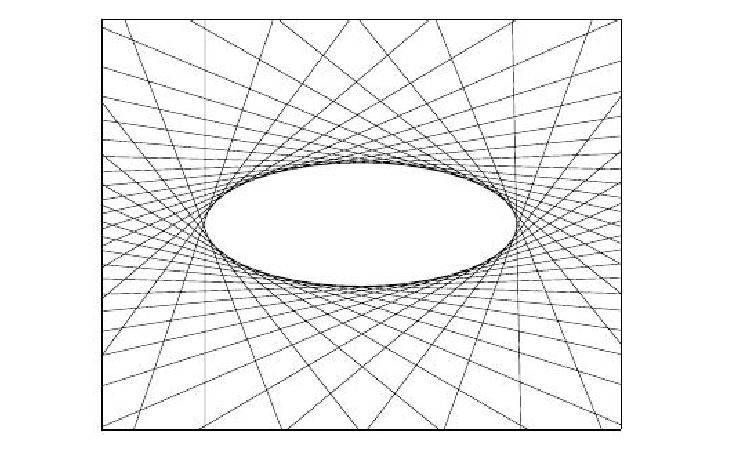
\includegraphics[scale=1]{conica-envelope}
\caption{\textit{A cônica $C$ é o envelope de todas as retas $\lightrgb_i$ que satisfazem $\lightrgb^\top C^*\,\lightrgb=0$.}}
\label{fig.conica-envelope}
\end{figure}

\subsubsection{Cônicas degeneradas.}

Acontece quando a matriz não tem posto completo, daí a cônica será duas retas caso a matriz tenha posto $2$ ou uma reta repetida caso a matriz tenha posto $1$. A seguir dois exemplos de cônicas degeneradas, uma cônica ponto e uma cônica dual. A cônica 

\begin{equation*}
C=\lightrgb\,{\bf m}^\top+{\bf m}\,\lightrgb^\top
\end{equation*}
é uma cônica ponto composta por duas retas $\lightrgb$ e ${\bf m}$. Assim, se um ponto $\x\in\lightrgb$ então $\lightrgb^\top\x=0$ e esse ponto deve satisfazer $\x^\top C\,\x=0$. Portanto

\begin{equation*}
\begin{array}{rcl}
\x^\top C\,\x&=&\x^\top(\lightrgb\,{\bf m}^\top+{\bf m}\,\lightrgb^\top)\,\x\\
&=&\x^\top\lightrgb\,{\bf m}^\top\x+\x^\top {\bf m}\,\lightrgb^\top\x\\
&=&0\,{\bf m}^\top\x+\x^\top{\bf m}\,0\\
&=&0.
\end{array}
\end{equation*}
A argumentação é analoga caso $\x\in{\bf m}$. Uma cônica dual degenerada é formada por pontos e tem posto 2 caso seja composta por dois pontos, ou posto 1 caso seja composta por um ponto repetido, 

\begin{equation*}
C^*=\x\,\y^\top+\y\,\x^\top.
\end{equation*}
De forma análoga à argumentação anterior podemos demosntrar que $C^*$ define um equação em retas,

\begin{equation*}
\lightrgb^\top\,C^*\lightrgb=0.
\end{equation*}

\subsubsection{A Relação Polo-Polar.}\label{sec.polo-polar}

Vimos anteriormente que uma reta $\lightrgb$ é tangente a uma cônica num ponto $\x$ se 

\begin{equation*}
\lightrgb=C\,\x.
\end{equation*}
Mas se o ponto $\x$ não pertence à cônica $C$ então temos uma relação denominada \textit{polo-polar}, onde a reta $\lightrgb$ é chamada reta \textit{polar} de $\x$, e $\x$ é chamado o \textit{polo} da reta $\lightrgb$, conforme a ilustração na figura \ref{fig.polo-polar}.

A reta polar $\lightrgb=C\,\x$ intersecta a cônica 
$C$ em dois pontos $\y_1$ e $\y_2$, e as retas tangentes à cônica $C$ nesses dois pontos se intersectam em $\x$. Pois, considere o ponto $\y_1 \in C$ e a reta tangente a esse ponto ${\bf m}=C\,\y_1$. Essa tangente contém o ponto $\x$ se 

\begin{equation*}
\x^\top{\bf m}=0\qquad\text{ou}\qquad\x^\top C\,\y_1=0,
\end{equation*}  
e, usando a simetria da cônica $C$ e aplicando a transposição em $\x^\top C$, temos

\begin{equation*}
\x^\top C\,\y_1=(C\,\x)^\top\y_1=0,
\end{equation*}
mostando que o ponto $\y_1$ pertence à reta $\lightrgb=C\,\x$. Assim, a reta $\lightrgb$ intersecta a cônica $C$ no ponto $\y_1$, no qual a tangente à $C$ contém o ponto $\x$. Observe que se o ponto $\x$ se aproxima da cônica $C$, os dois pontos $\y_1$ e $\y_2$ vão se aproximando um do outro, e quando ponto $\x$ pertence à conica $C$ a reta polar se torna a reta tangente. O argumento é análogo para $\y_2$.\\


\begin{figure}[!htb]
\centering
\subfloat[]{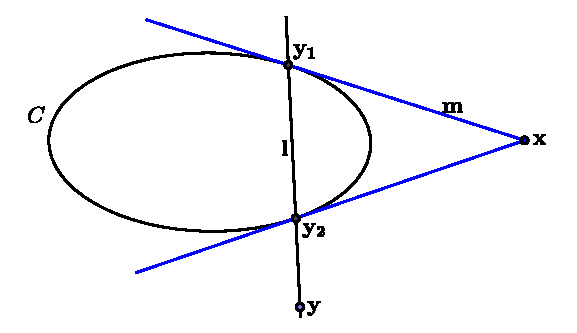
\includegraphics[scale=.81]{polo-polar}}
\quad
\subfloat[]{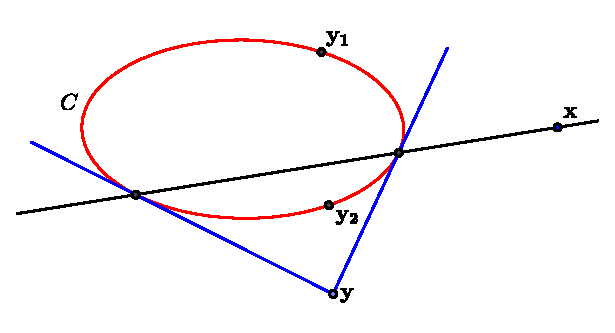
\includegraphics[scale=.81]{polo-polar-simetria}}
\caption{\textit{(a) A reta $\lightrgb=C\,\x$ é a reta polar de $\x$, e o ponto $\x=C^{-1}\lightrgb$ é o polo da reta $\lightrgb$. Os pontos $\x$ e $\y$ são chamados conjugados, pois obedecem à relação $\y^\top C\,\x=0$. (b) Duplicação da figura para visualização da simetria da relação polo-polar. O ponto $\x$ pertence à reta polar de $\y$.}}
\label{fig.polo-polar}
\end{figure}






\noindent {\bf Pontos conjugados.}

Quando um ponto $\y$ qualquer pertence à reta polar $\lightrgb=C\,\x$ temos que 

\begin{equation*}
\y^\top\lightrgb=\y^\top C\,\x=0,
\end{equation*}
e quaisquer dois pontos que satisfazem a relação $\y^\top C\,\x=0$ são chamados \textit{conjugados} com relação à cônica $C$. Repare que o ponto $y$ não precisa necessariamente pertencer à cônica. Mais anida, se um ponto $\y$ está na reta polar de $\x$, então $\x$ está na reta polar de $\y$. Como vimos, se $\y$ está na reta polar de $\x$ vale a relação $\y^\top C\,\x=0$, e tomando a transposta temos que $\x^\top C\,\y=0$, pois $C$ é simétrica. 
%Existe uma relacao de conjugacao para retas, digamos ${\bf l}$ e ${\bf m}$: ${\bf l}^\top C^*{\bf m}=0$.


\subsubsection{Transformação Projetiva em $\mathbb{P}^2$}\label{sec.trans-proj-H}

A tranformação projetiva também conhecida como projetividade, colineação ou homografia,  é um mapeamento (invertível) que transforma pontos no plano $\mathbb{P}^2$ para pontos no plano $\mathbb{P}^2$ preservando a colinearidade desses pontos. Mais formalmente, um mapeamento $h:\mathbb{P}^2\rightarrow\mathbb{P}^2$ é uma transformação projetiva se, e somente se, existe uma matriz $H_{3\times3}$ onde para cada ponto $\x\in\mathbb{P}^2$ temos que $h(\x)=H\,\x$. De fato, dados três pontos $\x_1$, $\x_2$ e $\x_3$ na mesma reta $\lightrgb$, temos que $\lightrgb^\top\x_i=0$ para $i=1,2 \,\,\,\text{e}\,\,\, 3$. Seja dada ainda $H_{3\times3}$ uma matriz invertível.

Definindo

\begin{equation*}
\lightrgb'=H^{-\top}\lightrgb \qquad\text{e}\qquad \x'_i=H\,\x_i,
\end{equation*}
vemos que todos os pontos $\x'_i$ pertencem à reta $\lightrgb'$, pois

\begin{equation*}
\begin{array}{rcl}
\lightrgb'^\top\x'_i&=&(H^{-\top}\lightrgb)^\top H\,\x_i\\
&=&\lightrgb^\top H^{-1}H\,\x_i\\
&=&\lightrgb^\top\x_i=0
\end{array}
\end{equation*}
preservando assim, a colinearidade dos pontos. A implicação contrária é demasiadamente grande. A argumentação mostra que qualquer transformação linear aplicada a coordenadas homogêneas é uma transformação projetiva em $\mathbb{P}^2$, ou seja, a transformação projetiva é simplesmente uma transformação linear em $\mathbb{R}^3$. Podemos ver que o efeito da matriz $H$ não é alterado pela multiplicação por um escalar diferente de zero na equação

\begin{equation*}
\x'=H\,\x,
\end{equation*}
pois os pontos permanecem colineares após a transformação, alterando apenas a escala. Assim, a matriz $H$ é chamada homogênea, e apenas a razão entre os seus elementos é significante. São nove elementos com oito graus de liberdade.\\

\noindent {\bf Transformação de retas.}

Na argumentação anterior vimos que a reta $\lightrgb'$ foi definida na forma $\lightrgb'=H^{-\top}\lightrgb$ e tal definição não foi à toa. Pois a definição nesta forma garante que os pontos depois de transformados permanecem colineares. Assim, a transformação projetiva de pontos nos dá essa regra para transformação projetiva de retas.\\

\noindent {\bf Transformação de cônicas.}

Invertendo o mapeamento $\x'=H\,\x$ temos que $\x=H^{-1}\x'$, e substituindo $\x$ na equação matricial de uma cônica $\x^\top C\,\x=0$:

\begin{equation*}
\begin{array}{rcl}
\x^\top C\,\x&=&(H^{-1}\x')^\top C\,H^{-1}\x'\\
&=&\x'^\top H^{-\top}C\,H^{-1}\x'\\
&=&\x'^\top C'\x'=0
\end{array}
\end{equation*}
onde $\x'^\top C'\x'=0$ é a equação matricial da cônica depois de aplicada a transformação projetiva, com $C'=H^{-\top}C\,H^{-1}$ sendo a regra para a transformação de cônicas.


\subsection{O Espaço Projetivo em Três Dimensões}\label{sec.espaco-P3}


\subsubsection{O Ponto} 


Analogamente à representação de um ponto no espaço $\mathbb{P}^2$, um ponto no espaço $\mathbb{P}^3$ é repesentado através de coordenadas homogêneas, acrescentando-se uma quarta coordenada ao vetor que representa esse ponto. Desta forma, $\X = (X_1,X_2,X_3,X_4)^\top$ e $X_4 \ne 0$, onde $\X$ é a representação em coordenadas homogêneas do ponto $(X,Y,Z)^\top \in \mathbb{R}^3$. Portanto esse vetor continua tendo três graus de liberdade. Para realizar tal mudança basta tomar 

\begin{equation*}
X=X_1/X_4 \,\, ,\, Y=X_2/X_4 \,\,\, \text{e} \,\,\, Z=X_3/X_4.
\end{equation*}

 

\subsubsection{ O Plano}

Temos que a representação algébrica de um plano $\bpi$ no espaço $\mathbb{R}^3$ é dada pela equação

\begin{equation*}
\pi_1\,X+\pi_2\,Y+\pi_3\,Z+\pi_4=0,
\end{equation*}
onde $\pi_i$ são os coeficientes da equação.

Um ponto em $\mathbb{R}^3$ pertence ao plano se, e somente se, satifaz a equação acima que na forma matricial usando a representação do ponto em coordenadas homogêneas fica:

\begin{center}
$
\begin{array}{ccc}
  (\pi_1,\pi_2,\pi_3,\pi_4)^\top
& \begin{pmatrix}
  X\\
  Y\\
  Z\\
  1
  \end{pmatrix}
& = 0.
\end{array}
$
\end{center}

Fazendo as substituições 
\begin{equation*}
X=X_1/X_4 \,\, , \,\, Y=X_2/X_4 \,\,\,\, \text{e} \,\,\,\, Z=X_3/X_4 ,
\end{equation*}

generalizamos a representação do ponto e a equação se torna:

\begin{center}
$
\begin{array}{ccccc}
(\pi_1,\pi_2,\pi_3,\pi_4)^\top
& \begin{pmatrix}
  X_1\\
  X_2\\
  X_3\\
  X_4
  \end{pmatrix}
& = 0
& \qquad \text{ou} \qquad
& \bpi^\top \, \X = 0.
\end{array}
$
\end{center}


Desta forma, verificamos que, assim como os pontos, um plano $\bpi = (\pi_1,\pi_2,\pi_3,\pi_4)^\top$ fica inteiramente determinado por um vetor com quatro coordenadas em $\mathbb{P}^3$. Aqui temos uma analogia com o espaço $\mathbb{P}^2$, já que pontos e retas têm a mesma representação vetorial com três coordenadas naquele espaço. Como multiplicar a equação algébrica de um plano por um escalar diferente de zero não altera seu valor, temos que os planos possuem três graus de liberdade. Podemos dividir as três primeiras coordenadas pela última, por exemplo, e fixar um escala.

Obs: As três primeiras coordenadas do vetor que representa o plano corresponde ao vetor normal ao plano, conforme definido em Álgebra Linear.
\\


\subsubsection{A Reta}

Uma reta pode ser definida passando por dois pontos. Em $\mathbb{P}^2$, como os dois pontos estão no mesmo plano, uma reta passando por esses dois pontos tem apenas três graus de liberdade, conforme visto anteriormente. Mas em $\mathbb{P}^3$, como os dois pontos podem estar em planos diferentes, temos que uma reta apresenta quatro graus de liberdade, dois graus para cada ponto. Assim, uma reta deveria ser representada por um vetor com cinco coordenadas em $\mathbb{P}^3$, mas vetores desse tipo não podem ser usados, facilmente, em expressões matemáticas que envolvem vetores com quatro coordenadas representando pontos e planos. Portanto é necessário encontrar uma outra representação, e uma das formas mais simples é definir a reta através de dois pontos não coincidentes. Outras representações de uma reta no espaço projetivo $\mathbb{P}^3$, diferentes da apresentada aqui, podem ser encontradas em \cite{Hartley2004}.


Uma reta ${\bf L}$ passando por dois pontos ${\bf A} \,\,\, \text{e} \,\,\, {\bf B}$ é representada pelo espaço linha gerado pela matriz $W$ composta pelos pontos ${\bf A}^\top \,\,\,\text{e} \,\,\, {\bf B}^\top$ em linha:

\begin{center}
$
\begin{array}{cc}
W = 
& \begin{bmatrix}
  A^\top\\
  B^\top
  \end{bmatrix},
\end{array}
$
\end{center}
onde os espaço gerado por $W^\top$ é o conjunto de pontos do tipo $a\,{\bf A} + b\,{\bf B}$ pertencentes à reta ${\bf L}$ procurada. \\


\subsubsection{A Quádrica}


Similarmente à cônica em $\mathbb{P}^2$, uma quádrica $Q$ em $\mathbb{P}^3$ é definida pela equação

\begin{equation*}
\X^\top\,Q\,\X = 0,
\end{equation*}
onde $Q$ é uma matriz simétrica $4\times4$ com nove graus de liberdade.




\begin{figure}[!htb]
$
\begin{array}{cc}
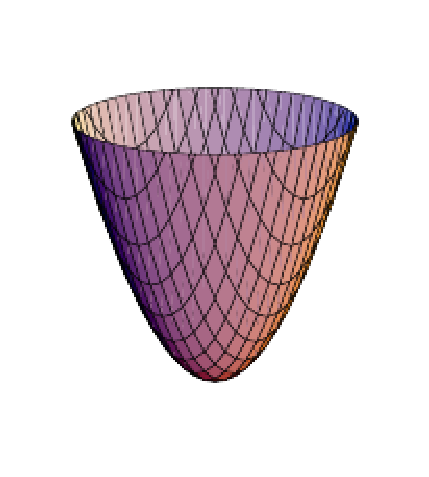
\includegraphics[scale=1.1]{paraboloide}
&
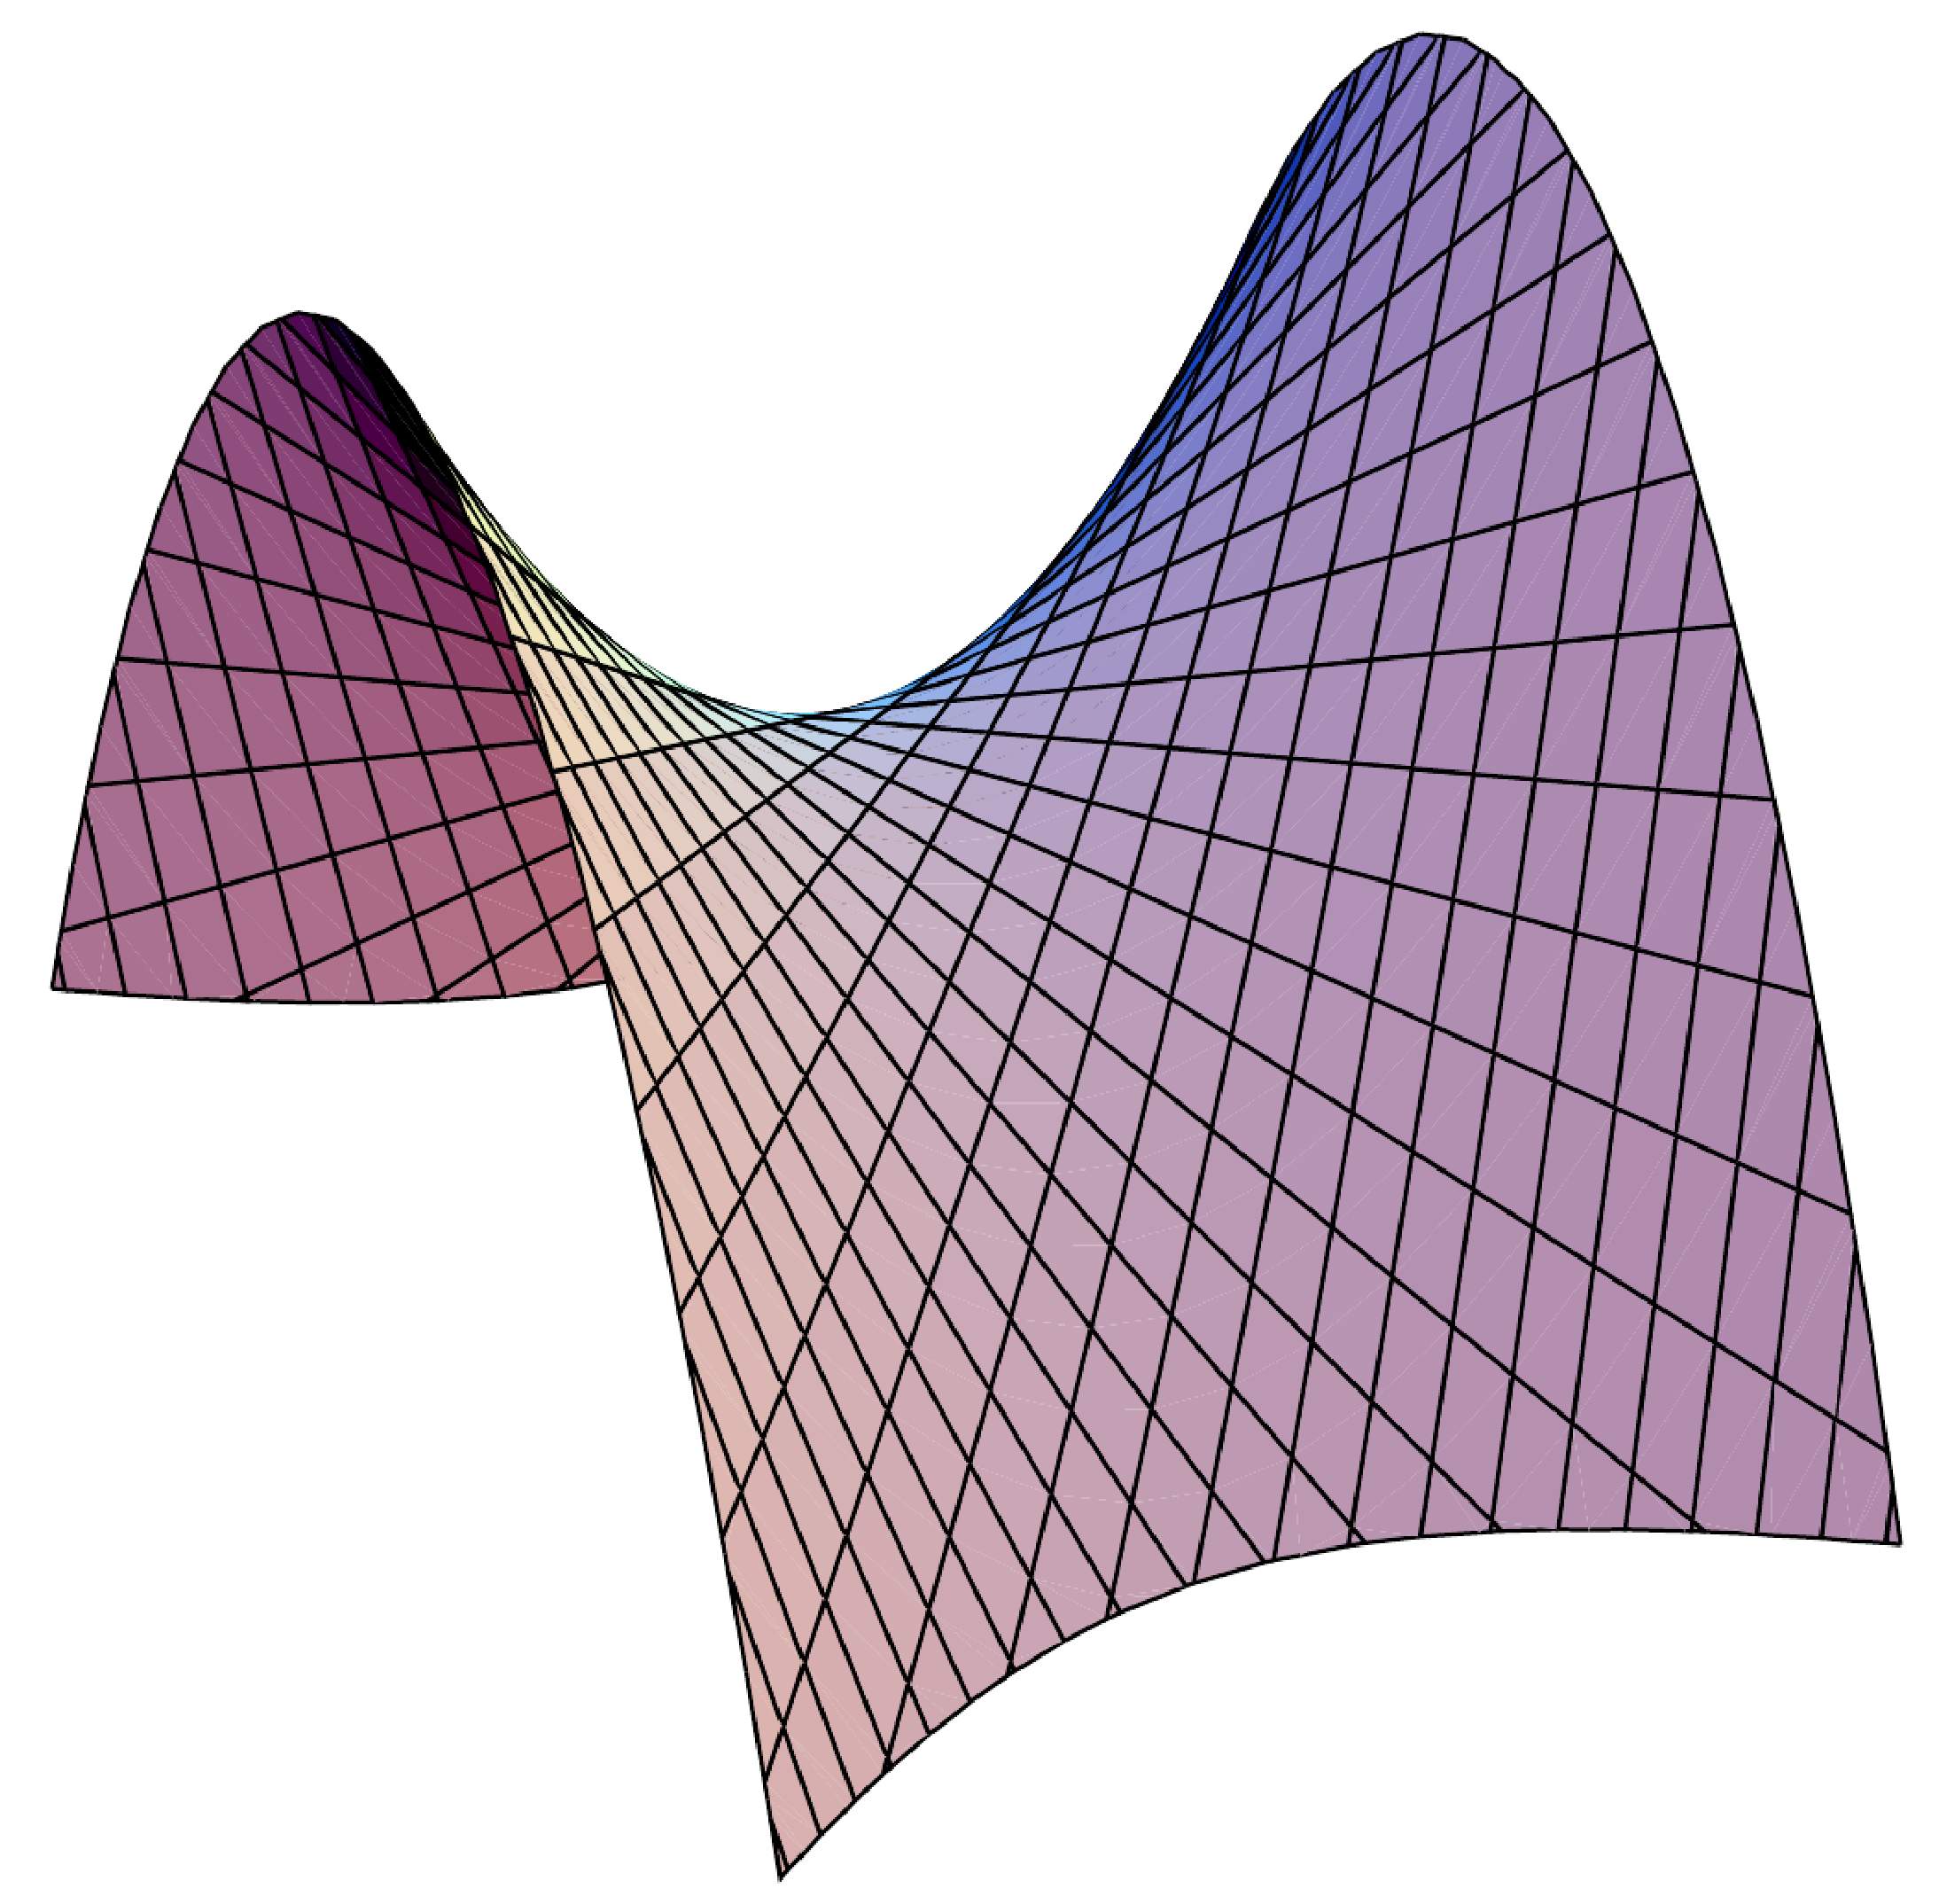
\includegraphics[scale=0.9]{hiperboloide_1_folha}
\end{array}
$
\caption{\textit{Parabolóide à esquerda e hiperbolóide de uma folha à direita.}}
\label{quadricas}
\end{figure}


Mais detalhes sobre a dedução da definição de uma quádrica podem ser encontrados em \cite{Hartley2004}, bem como outros exemplos além daqueles observados na figura \ref{quadricas}.\\

\subsubsection{A transformação de pontos e planos em $\mathbb{P}^3$.}

A transformação de pontos e planos em $\mathbb{P}^3$ é inteiramente análoga àquela argumentada na subseção \ref{sec.espaco-P2} para pontos e retas em $\mathbb{P}^2$, pois assim como os pontos têm uma relação dual com retas em $\mathbb{P}^2$, os pontos também têm uma relação dual com planos em $\mathbb{P}^3$ e, como vimos, ambos têm a mesma representação em vetores homogêneos com quatro componentes. Assim, sob uma tranformação projetiva de pontos $\X'=H\,\X$ temos que planos se transformam de acordo com

\begin{equation*}
\bpi'=H^{-\top}\bpi.
\end{equation*}







\subsubsection{Direções e o plano no infinito.}

O plano no infinito é denotado por $\bpi_\infty$, tem a foma canônica $\bpi_\infty=(0,0,0,1)^\top$ e é composto por pontos no infinito $D=(x_1,x_2,x_3,0)^\top$ que são as direções das retas contidas no espaço. No espaço projetivo $\mathbb{P}^2$ duas retas paralelas se encontram num ponto no infinito, e analogamente, em  $\mathbb{P}^3$ dois planos paralelos se encontram numa reta que está contida no plano no infinito, e também, uma reta é paralela a outra reta (ou a um plano) se o ponto de interseção está no $\bpi_\infty$. O plano no infinito é invariável sob uma transformação afim.

De acordo com a subseção \ref{sec.espaco-P3} temos que a transformação projetiva de planos no espaço  $\mathbb{P}^3$ se dá pela fórmula $\bpi'=H^{-\top}\bpi$, assim podemos verificar porque um plano no infinito é invariante sob a tranformação afim. Conforme a subseção tal vimos que a transformação afim é dada por 

\begin{equation*}
H_A=
\begin{bmatrix}
A&{\bf t}\\
{\bf 0}^\top&1
\end{bmatrix},
\end{equation*}
então

\begin{equation*}
H_A^{-\top}=
\begin{bmatrix}
A^{-\top}&{\bf 0}\\
-{\bf t}^\top A^{-\top}&1
\end{bmatrix},
\end{equation*}
e aplicando ao plano no infinito temos:

\begin{equation*}
\begin{array}{rcl}
\bpi'&=&H_A^{-\top}\bpi_\infty\\
&=&
\begin{bmatrix}
A^{-\top}&{\bf 0}\\
-{\bf t}^\top A^{-\top}&1
\end{bmatrix}\,
\begin{pmatrix}
0\\
0\\
0\\
1
\end{pmatrix}\\
&=&
\begin{pmatrix}
0&0&0&1
\end{pmatrix}^\top\\
&=&
\bpi_\infty.
\end{array}
\end{equation*}
Existem outros planos que podem ser invariáveis sob uma transformação afim menos específica, mas só o plano no ifinito é invariável em uma transformação afim geral. Cabe resaltar que $\bpi_\infty$ é invariável apenas quando a transformação é aplicada ao conjunto, e não a pontos isolados pertencentes a esse plano.


\subsubsection{A cônica absoluta.}\label{sec.con-absoluta}

A cônica absoluta é uma cônica (ponto) denotada por $\Omega_\infty$ e está contida no plano no infinito $\bpi_\infty$. Em coordenadas Euclidianas o plano no infinito tem definição $\bpi_\infty=(0,0,0,1)$ e a cônica absoluta é definida através da equação matricial

\begin{equation*}
\X^\top\Omega_\infty\X=0,
\end{equation*} 
onde as componentes de $\X$ obedecem às restrições

\begin{equation*}
X_1^2+X_2^2+X_3^2=0\qquad\text{e}\qquad\,X_4=0.
\end{equation*}
De acordo com essas restrições e com esse sistema de coordenadas, e para satisfazer a equação matrical da cônica, temos que $\Omega_\infty=I_{3\times3}$, pois

\begin{equation*}
(X_1,X_2,X_3)\,I\,(X_1,X_2,X_3)^\top=0.
\end{equation*}

Da mesma forma que o plano no infinito é invariável sob uma transformação afim, a cônica absoluta é invariável sob uma transformação de similaridade. Já que a cônica absoluta está contida no plano no infinito, a transformação afim que mantem fixo esse plano também deverá manter invariável as coordenadas da cônica, sendo então a cônica absoluta invariável sob uma transformação afim

\begin{equation*}
H_A=
\begin{bmatrix}
A&{\bf t}\\
{\bf 0}^\top&1
\end{bmatrix}.
\end{equation*}
Aplicando a homografia afim $H_A$ aos pontos da cônica absoluta temos que as três primeiras componentes desses pontos são afetadas apenas pela submatriz $A_{3\times3}$,

\begin{equation*}
\begin{bmatrix}
A&{\bf t}\\
{\bf 0}^\top&1
\end{bmatrix}
\begin{pmatrix}
X_1\\
X_2\\
X_3\\
0
\end{pmatrix}
=
\begin{pmatrix}
A\,
\begin{pmatrix}
X_1\\
X_2\\
X_3
\end{pmatrix}\\
0
\end{pmatrix}.
\end{equation*}
Como vimos, essas três primeiras componentes são utilizadas na definição da cônica absoluta, e portanto $\Omega_\infty$ vai sofrer influência apenas de $A$ em tal transformação. 
De acordo com a tranformação de cônicas na subseção \ref{sec.trans-proj-H}, e com o fato de $\Omega_\infty$ ser invariável sob 
$H_A$, temos que $A^\top I A^{-1}=I$, assim

\begin{equation*}
\begin{array}{rcl}
I&=&A^{-\top}I\,A^{-1}\\
&=&A^{-\top}A^{-1}\qquad\text{tomando a inversa}\\
&=&A\,A^\top.
\end{array}
\end{equation*}
Desta forma percebemos que $A$ é uma matriz ortogonal (possivelmente com aplicação de escala), o que está de acordo com a definição de tranformação de similaridade $H_S$ conforme a subseção tal.

\subsubsection{A quádrica dual absoluta.}\label{sec.quadrica-dual-abs}
A quádrica dual absouta é a dual degenerada da cônica absoluta $\Omega_\infty$, e é denotada por 
${\tt Q}^*_\infty$. Analogamente ao fato de que o envelope da cônica dual $C^*$ é composto pelas retas tangentes à cônica $C$ no ${\mathbb{P}}^2$, temos que, geometricamente,  o envelope da quádrica dual absoluta é composto de todos os planos que são tangentes à cônica absoluta. Algebricamente, 
${\tt Q}^*_\infty$ é representada por uma matriz homogênea $4\times4$ e num sistema de coordenadas métrico tem a forma canônica

\begin{equation}\label{eq.quadrica-dual-abs}
{\tt Q}^*_\infty=
\begin{bmatrix}
1&0&0&0\\
0&1&0&0\\
0&0&1&0\\
0&0&0&0
\end{bmatrix}=
\begin{bmatrix}
I&{\bf 0}\\
{\bf 0}^\top&0
\end{bmatrix}.
\end{equation}
Para ver que os planos envelopados pela quádrica dual absoluta ${\tt Q}^*_\infty$ são tangentes à cônica absoluta $\Omega_\infty$, considere um plano $\bpi=({\bf v}, k)^\top$. Esse plano está no envelope definido por ${\tt Q}^*_\infty$ se, por definição, $\bpi^\top {\tt Q}^*_\infty\bpi=0$. Usando a definição em \ref{eq.quadrica-dual-abs} temos

\begin{equation*}
\begin{array}{rcl}
\bpi^\top {\tt Q}^*_\infty\bpi&=&
\begin{pmatrix}
{\bf v}^\top&k
\end{pmatrix}
\begin{bmatrix}
I&{\bf 0}\\
{\bf 0}^\top&0
\end{bmatrix}
\begin{pmatrix}
{\bf v}\\
k
\end{pmatrix}\\
&=&{\bf v}^\top {\bf v}\\
&=&0,
\end{array}
\end{equation*}
onde, ${\bf v}$ representa a reta de interseção do plano $\bpi$ com o plano no infinito $\bpi_\infty$. De acordo com as subseções \ref{sec.espaco-P2} e \ref{sec.con-absoluta}, a reta ${\bf v}$ que pertence ao plano no infinito, é tangente à cônica absoluta se, e somente se, ${\bf v}^\top I\,{\bf v}=0$. Portanto, o envelope de ${\tt Q}^*_\infty$ é composto pelos planos que são tangentes à $\Omega_\infty$. 

Para ver que ${\bf v}$ é a reta de interseção de $\bpi$ com $\bpi_\infty$, considere o sistema abaixo onde um ponto $\X$ pertence a esses dois planos. Esse ponto pertence a cada um dos planos se

\begin{empheq}[left=\empheqlbrace]{align*}
\begin{pmatrix}
{\bf v}^\top&k
\end{pmatrix}
\begin{pmatrix}
X_1\\
X_2\\
X_3\\
X_4
\end{pmatrix}
=0\\
\bpi^\top_\infty
\begin{pmatrix}
X_1\\
X_2\\
X_3\\
X_4
\end{pmatrix}
=0.
\end{empheq}
Pela segunda equação, como $\bpi=(0,0,0,1)$ temos que $X_4=0$ (o que já não era novidade). Substituindo $X_4=0$ na primeira equação e efetuando a multiplicação matricial, a constante $k$ desaparece multiplicada por zero e restará

\begin{equation*}
{\bf v}^\top
\begin{pmatrix}
X_1\\
X_2\\
X_3
\end{pmatrix}=0.
\end{equation*}
A última equação representa a equação de pertinência de um ponto a uma reta conforme as subseções \ref{sec.reta} e \ref{sec.ponto}. 


\subsection{A Câmera P}

A câmera é modelada como um dispositivo que mapeia um ponto no sistema de coordenadas do mundo em pontos no sistema de coordenadas da imagem. Matematicamente, a \textit{câmera} é uma transformação linear entre um ponto 3D no espaço e um ponto 2D no plano da imagem, representada por uma matriz com algumas propriedades que realizam o mapeamento entre os pontos. Existem vários tipos de câmera, mas para tratar das características básicas vamos utilizar o modelo buraco de alfinete, do inglês \textit{pinhole}.
\\
Esse tipo de câmera é uma composição de três mudanças de coordenadas, representada por uma matriz $P$ que pode ser decomposta em:

\begin{equation*}
P = K \, [I|{\bf 0}]
\begin{bmatrix}
R&{\bf t}\\
\,\,{\bf 0}^\top &1
\end{bmatrix}
= K\,[R|{\bf t}],
\end{equation*}
onde 

\begin{itemize}
\item a matriz $\begin{bmatrix}
R&{\bf t}\\
\,\,{\bf 0}^\top &1
\end{bmatrix}$
contendo os parâmetros extrínsecos transforma os pontos em coordenadas 3D no mundo para as coordenadas 3D da câmera.
\item a matriz $[I|{\bf 0}]$ aplica a projeção perpectiva passando um ponto na coordenada 3D da câmera para um ponto 2D em coordenadas normalizadas no plano da imagem.
\item a matriz $K$, matriz de calibração contendo os parâmetros intrínsecos, transforma pontos em coordenadas normalizadas no plano da imagem para as coordenadas na imagem ``final" (considerando mudanças como medida em pixels, por exemplo).  
\end{itemize}
Mais a frente vamos abordar cada um desses tópicos com mais detalhes.

Para fazermos a construção da câmera, consideramos o \textit{centro de projeção}, ou \textit{centro da câmera}, como a origem do espaço tridimensional Euclidiano, com o \textit{plano da imagem} ou \textit{plano focal} sendo $Z = f$, onde $f$ é a \textit{distancia focal} entre o plano da imagem e o centro de projeção. Assim, o plano da imagem é definido como $(x,y,f)^\top$ mas seu sistema de coordenadas é medido em pixels e é centralizado no canto inferior esquerdo da imagem. Por \textit{coordenadas normalizadas da imagem} nos referimos aos pontos $(x,y)^\top$ expressos como $(x,y,1)^\top$ (considerando que a câmera tenha distância focal unitária)no plano da imagem com relação ao sistema de coordenadas da câmera. O \textit{plano detector} fica em $(x,y,-f)^\top$. Como podemos obeservar na figura \ref{camera}, um ponto $\X$ no espaço 3D é mapeado a um ponto $\x$ no plano da imagem por uma reta que liga $\X$ ao centro de projeção, e intersepta o plano da imagem. Assim, ignorando a última coordenada homogênea do vetor que representa o ponto na imagem, temos o mapeamento:

\begin{center}
$\X = (X,Y,Z)^\top \rightarrow \x = (fX/Z,fY/Z,f) \rightarrow (fX/Z,fY/Z)$  
\end{center}

O plano que passa pelo centro da câmera e é paralelo ao plano da imagem é chamado \textit{plano principal}, o plano $xy$ na figura \ref{camera}. O \textit{eixo principal} passa pelo centro da câmera e é perpendicular ao plano da imagem, onde a interseção desse eixo com o plano da imagem forma o \textit{ponto principal}, o qual pode ser pensado como a projeção do centro da câmera no plano da imagem.


\begin{figure}[!htb]
\centering
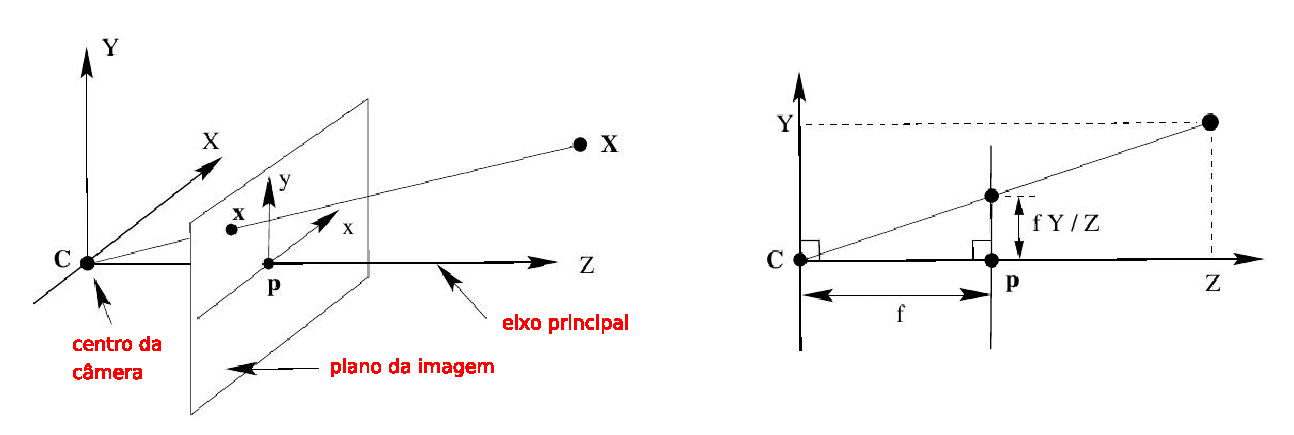
\includegraphics[scale=.75]{modelo_camera}
\caption{\textit{Visualização das características básicas de uma câmera como distância focal, eixo principal, plano da imagem, centro de projeção e o ponto principal {\bf P}.}}
\label{camera}
\end{figure}

Com vetores representados em coordenadas homogêneas, podemos expressar o mapeamento através de um operador linear, onde realizamos a multiplicação da matriz $P$, que representa a câmera, por um ponto no espaço, resultando num ponto na imagem conforme o esquema abaixo:

\begin{center}
$
\begin{array}{ccc}
\begin{pmatrix}
fX\\
fY\\
Z
\end{pmatrix} = 
&
\begin{bmatrix}
f& & &0\\
 &f& &0\\
 & &1&0
\end{bmatrix}
&
\begin{pmatrix}
X\\
Y\\
Z\\
1
\end{pmatrix}
\end{array}
$
\end{center}

Nessa matriz temos que $f$ é a distância focal (entre o centro da câmera e o plano da imagem), e o vetor de coluna de zeros à direita representa as coordenadas do centro da câmera, que nesse caso está na origem do sistema. Essa matriz pode ser desmembrada da seguinte maneria: uma matriz diagonal $diag(f,f,1)$ multiplicada pela matriz $[I|{\bf 0}]$, onde $I$ é uma matriz identidade $3\times3$ e ${\bf 0}$ é um vetor coluna de zeros. Compactamente, podemos escrever a ultima relaçao como:

\begin{center}
$\x = diag(f,f,1)\,[I|{\bf 0}]\,\X$,
\end{center}
onde $diag(f,f,1)\,[I|{\bf 0}]$ é a matriz da câmera para o modelo \textit{pinhole}.

Nessa dedução, consideramos que o ponto principal  coincide com a origem do plano da imagem, mas na prática isso pode não acontecer. Dessa forma, devemos acrescentar as coordenadas do ponto na construção da matriz da câmera. Sendo $(p_x,p_y)$ as coordenadas do ponto principal, desejamos o seguinte mapeamento:

\begin{center}
$(X,Y,Z)^\top \rightarrow (\frac{f\,X}{Z}+p_x\,,\,\frac{f\,Y}{Z}+p_y)$,
\end{center}
o qual nos fornece a seguinte relação de projeção em coordenadas homogêneas:

\begin{center}
$
\begin{array}{ccc}
\begin{pmatrix}
f\,X + Z\,p_x\\
f\,Y + Z\,p_y\\
Z
\end{pmatrix}=
&
\begin{bmatrix}
f& &p_x&0\\
 &f&p_y&0\\
 & &1&0
\end{bmatrix}
\begin{pmatrix}
X\\
Y\\
Z\\
1
\end{pmatrix}
\end{array}
$
\end{center}

Definindo a notação

\begin{center}
$
\begin{array}{cc}
K = & \begin{bmatrix}
      f& &p_x\\
       &f&p_y\\
       & &1
      \end{bmatrix}, 
\end{array}
$
\end{center}
a relação de projeção assume a forma


\begin{equation}
\x=K\,[I|{\bf 0}]\,\X_{\textit{cam}},
\end{equation}
onde $K$ é denominada matriz de calibração da câmera, a qual resume os parâmetros internos da mesma, e $\X_{\textit{cam}}$ enfatiza que o ponto 3D está escrito no sistema de coordenadas da câmera.

A matriz de calibração $K$ ainda não está completa, pois o sistema de coordenadas do plano da imagem é medido em pixels, que podem não ser quadrados, e além disso os eixos cartesianos desse sistema podem não ser ortogonais. Assim, vamos inserir mais dois parâmetros para definir a medição em pixels e mais um parâmetro para definir o ângulo de inclinação entre os eixos cartesianos.

Sendo $m_x$ e $m_y$ a quantidade de pixels nas direções $x$ e $y$, respectivamente, a transformação para a coordenadas em pixels se dá pela multiplicação da matriz $diag(m_x,m_y,1)$ à esqueda da matriz $K$,
\begin{equation*}
\begin{bmatrix}
m_x&0&0\\
0&m_y&0\\
0&0&1
\end{bmatrix}      
\begin{bmatrix}
f& &p_x\\
&f&p_y\\
& &1
\end{bmatrix}
=
\begin{bmatrix}
\alpha_x&0&x_0\\
0&\alpha_y&y_0\\
0&0&1
\end{bmatrix}
\end{equation*}
onde $\alpha_x=m_x\,f$, $\alpha_y=m_y\,f$ representa a distância focal em termos das dimensões dos pixels. Similarmente, $x_0=m_x\,p_x$ e $y_0=m_y\,p_y$ são as coordenadas do ponto principal medidas em pixels.

Para completar a generalidade, acrescentamos o parâmetro $s$, referente à inclinação entre os eixos, na matriz
\begin{equation*}
K=
\begin{bmatrix}
\alpha_x&s&x_0\\
0&\alpha_y&y_0\\
0&0&1
\end{bmatrix}.
\end{equation*}






Até aqui temos expressado o ponto $\X$ no espaço em relação às coordenadas da câmera, assumindo que o centro da câmera está situado na origem do sistema de eixos, o qual recebe o nome de sistema de coordenadas da câmera. Mas na maioria das vezes esse não é o caso, portanto desejamos fazer o mapeamento de um ponto 3D cujo as coordenadas estejam expressas com relação a um sistema de coordenadas qualquer, chamado sistema de coordenadas do mundo. Portanto, vamos continuar completando a matriz $P$ para mapear pontos no sistema de coordenadas do mundo.

Considerando o sistema de coordenadas do mundo, denotaremos um ponto nesse sistema, em coordenadas não homogêneas, por $\overline{\X}$, e o mesmo ponto no sistema de coordenadas da câmera será denotado por $\overline{\X}_{\textit{cam}}$. A transferência de sistemas de coordenadas é feita através da relação $\overline{\X}_{\textit{cam}}=R\,(\overline{\X}-\overline{\bf C})$, onde $\overline{\bf C}$ representa o centro da câmera no sistema de coordenadas do mundo e $R$ representa uma matriz de rotação $3\times3$. Passando os vetores para coordenadas homogêneas, podemos aplicar a rotação no vetor $\overline{\bf C}$, do centro da câmera, e inseri-lo na quarta coluna da matriz escrevendo a relação

\begin{center}
$
\begin{array}{ccc}
\overline{\X}_{\textit{cam}}=
&
\begin{bmatrix}
R&-R\,\overline{\bf C}\\
\,\,{\bf 0}^\top&\,\,1
\end{bmatrix}
&
\begin{pmatrix}
X\\
Y\\
Z\\
1
\end{pmatrix},
\end{array}
$
\end{center} 
onde podemos escrever

\begin{center}
$
\begin{array}{cccc}
R=
&
\begin{bmatrix}
a&b&c\\
d&e&f\\
g&h&i
\end{bmatrix}
&
\qquad\text{e}\qquad
&
-R\,\overline{\bf C}=(t_1,t_2,t_3)^\top,
\end{array}
$
\end{center}
e a relação acima fica:

\begin{center}
$
\begin{array}{ccc}
\overline{\X}_{\textit{cam}}=
&
\begin{bmatrix}
a&b&c&t_1\\
d&e&f&t_2\\
g&h&i&t_3\\
0&0&0&\,1
\end{bmatrix}
&
\begin{pmatrix}
X\\
Y\\
Z\\
1
\end{pmatrix}.
\end{array}
$
\end{center}

Substituindo $\overline{\X}_{\textit{cam}}$ em (1), obtemos

\begin{center}
$
\begin{array}{ccccc}
\x=
&
\begin{bmatrix}
\alpha_x&s&x_0\\
0&\alpha_y&y_0\\
0&0&1
\end{bmatrix}&
\begin{bmatrix}
1&0&0&0\\
0&1&0&0\\
0&0&1&0
\end{bmatrix}
&
\begin{bmatrix}
a&b&c&t_1\\
d&e&f&t_2\\
g&h&i&t_3\\
0&0&0&\,1
\end{bmatrix}
&
\begin{pmatrix}
X\\
Y\\
Z\\
1
\end{pmatrix},
\end{array}
$
\end{center}
multiplicando a segunda e terceira matrizes,
 
\begin{center}
$
\begin{array}{cccc}
\x=
&
\begin{bmatrix}
\alpha_x&s&x_0\\
0&\alpha_y&y_0\\
0&0&1
\end{bmatrix}&
\begin{bmatrix}
a&b&c&t_1\\
d&e&f&t_2\\
g&h&i&t_3
\end{bmatrix}
&
\begin{pmatrix}
X\\
Y\\
Z\\
1
\end{pmatrix},
\end{array}
$
\end{center}
que pode ser escrita de forma resumida como

\begin{center}
$
\x=K\,[R|{\bf t}]\,\X,
$
\end{center}
com ${\bf t}=(t_1,t_2,t_3)^\top$ denominado vetor de translação.

Acabamos de incluir todos os parâmetros na matriz $P=K\,[R|{\bf t}]$, para o mapeamento de um ponto 3D homogêneo no sistema de coordenadas do mundo em seu respectivo ponto 2D no plano da imagem, no sistema de coordenadas da imagem. Temos cinco parâmetros internos na matriz de calibração $K$, $(\alpha_x,\alpha_y,s,p_x,p_y)$, três parâmetros externos na matriz de rotação $R$, apesar de suas nove entradas, e mais três parâmetros externos no vetor de translação totalizando 11 graus de liberdade. Repare que, tendo a matriz $P$ dimensão $3\times4$, ela possui 12 componentes e, usando uma para determinar a escala, sobram exatamente os 11 graus de liberdade, e a câmera $P$ é chamda câmera de \textit{projeção finita}.

\subsubsection{A Matriz de Calibração K.}

A intenção nesta seção é mostrar qual é a natureza de cada um dos parâmetros internos da matriz de calibração. Para isso, vamos resolver o problema de transferir um ponto qualquer no espaço para o plano da imagem na câmera.

Dado um ponto 3D $p^w = (x^w,y^w,z^w)^\top$ em coordenadas do mundo e sendo $(\uu,\vv)$ as coordenadas do ponto na imagem da câmera, quais os valores de $(\uu,\vv)$?

Primeiramente, vamos transformar o ponto em coordenadas do mundo para as coordenadas da câmera $p = (x,y,z)^\top$:
\begin{align*}
p = R p^w + T
\end{align*}
onde $R$ e $T$ são parâmetros extrínsecos.

Agora, vamos projetar o ponto para o plano imagem normalizada usando similaridade de triângulos:
\begin{empheq}[left=\empheqlbrace]{align*}\label{eq:normalized:coords}
\tilde x = \frac{x}{z}\\
\tilde y = \frac{y}{z}
\end{empheq}

Depois dessa projeção, vamos aplicar os parâmetros internos para obtermos as coordenadas finais da imagem. O primeiro passo é incluir a distância focal.
\begin{empheq}[left=\empheqlbrace]{align*}
\tilde x &= f\frac{x}{z}\\
\tilde y &= f\frac{y}{z}
\end{empheq}
Então converter para pixels:
\begin{empheq}[left=\empheqlbrace]{align*}
\tilde x_{pix} &= s_\uu f\frac{x}{z}\\
\tilde y_{pix} &= s_\vv f\frac{y}{z}
\end{empheq}
Como podemos ver, $f$ tem efeito similar a $s_\uu$ e $s_\vv$. Seria suficiente mantermos apenas dois parâmetros, digamos $f$ e a razão de aspecto, mas vamos manter os três parâmetros por enquanto.
%
%
Em seguida, fazemos a translação para o ponto inferior esquerdo da imagem usando $(t_{\tilde \uu},t_{\tilde \vv})$, que são as coordenadas do ponto principal em relação ao inferior esquerdo da imagem:
\begin{empheq}[left=\empheqlbrace]{align*}
\tilde \uu &= s_\uu f\frac{x}{z} + t_{\tilde \uu}\\
\tilde \vv &= s_\vv f\frac{y}{z} + t_{\tilde \vv}
\end{empheq}

E convertemos para o sistema de coordenadas em função de um ângulo $\theta$ entre os eixos, pois os eixos podem ser não ortogonais. Observe na figura \ref{skew} a conversão das coordenadas de um ponto $Q$ qualquer:

\begin{figure}[!htb]
\centering
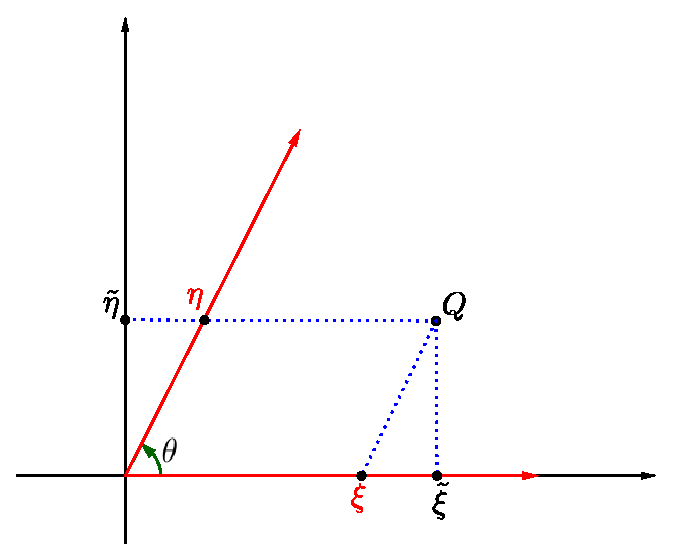
\includegraphics[scale=1]{skew}
\caption{\textit{Transformação das coordenadas de um ponto no plano com eixos perpendiculares para um plano com eixos relacionados por um ângulo $\theta$ qualquer.}}
\label{skew}
\end{figure}

\begin{empheq}[left=\empheqlbrace]{align*}
\tilde \uu &= \uu + \vv \, cos\,\theta
\\
\tilde \vv &= \vv \, sen\,\theta
\end{empheq}

Isolando as variáveis do sistema de coordenadas com ângulo genérico temos:


\begin{empheq}[left=\empheqlbrace]{align*}
\uu &= \tilde \uu - \tilde \vv \cot\theta \\
\vv &= \tilde \vv \,cossec\, \theta
\end{empheq}
os quais fornece
\begin{empheq}[left=\empheqlbrace]{align*}\label{eq:projection:explicit}
\uu &= \overbrace{s_\uu f}^{\alpha_\uu}\frac{x}{z} + \overbrace{(-\cot\theta\, s_\vv
f)}^{s_\theta} \frac{y}{z} + \overbrace{t_{\tilde \uu} - \cot\theta\, t_{\tilde \vv}}^{\uu_0}\\
%
\vv &= \underbrace{s_\vv f\,cossec\,\theta}_{\alpha_\vv} \frac{y}{z}+
\underbrace{cossec\,\theta\, t_{\tilde \vv}}_{\vv_0}
\end{empheq}
Assim, a transformação de um ponto na câmera para a imagem é feita usando cinco parâmetros da matriz de calibração $K$. A fórmula acima explicita a interpretação de cada um desses parâmetros.


\begin{table}
\begin{center}
\begin{tabular}{c l} 
\textbf{Variáveis Livres} & \textbf{Descrição}\\
3	 & rotação \\
3	 & translação \\
2	 & mudança de escala em $x,y$\\
1	 & distância focal (pode ser incorporada como escala)\\
2	 & ponto principal\\
1	 & ângulo entre os eixos \\
6  & total extrinsecos\\
6  & total intrinsecos\\
12 & total\\
11 & total único (distância focal para fixar escala)
\end{tabular}
\end{center}
\caption{Resumo dos parâmetros da câmera.}
\end{table}

\subsection{A ação projetiva de uma câmera $P$.}
Nesta subseção iremos verificar como se dá a projeção aplicada por uma câmera $P$ em planos, retas, cônicas e quádricas.


\subsubsection{Ação projetiva de $P$ em planos.}
A equação de projeção é uma transformação de um ponto em coordenadas 3D no sistema de coordenadas do mundo para pontos 2D no sistema de coordenadas do plano da imagem na câmera e, nessa estrutura, temos a liberdade para escolher o sistema de coordenadas do mundo. Assim, suponha que tal sistema de coordenadas seja posicionado de forma que o plano $xy$ corresponda ao plano $\bpi$, conforme ilustrado na figura \ref{fig.projecao-planos-retas}. Desta forma, pontos no espaço que pertencam ao plano $\bpi$ terão a componente $X_3=0$, e a ação de uma câmera $P$ nesses pontos é dada por

\begin{equation*}
\begin{array}{rcl}
\x&=&P\,\X\\
&=&
\begin{pmatrix}
{\bf p_1}&{\bf p_2}&{\bf p_3}&{\bf p_4}
\end{pmatrix}
\begin{pmatrix}
X_1\\
X_2\\
0\\
1
\end{pmatrix}\\
&=&
\begin{pmatrix}
{\bf p_1}&{\bf p_2}&{\bf p_4}
\end{pmatrix}
\begin{pmatrix}
X_1\\
X_2\\
1
\end{pmatrix},
\end{array}
\end{equation*}
onde ${\bf p_i}$ são as colunas da matriz $P$. Assim, a transformação de um ponto $\X_\pi=(X_1,X_2,1)^\top\in\bpi$ para um ponto na imagem é, em geral, uma homografia planar, ou uma transformação projetiva de plano a plano $\x=H\,\X_\pi$.


\begin{figure}[htb!]
\centering
\subfloat[]{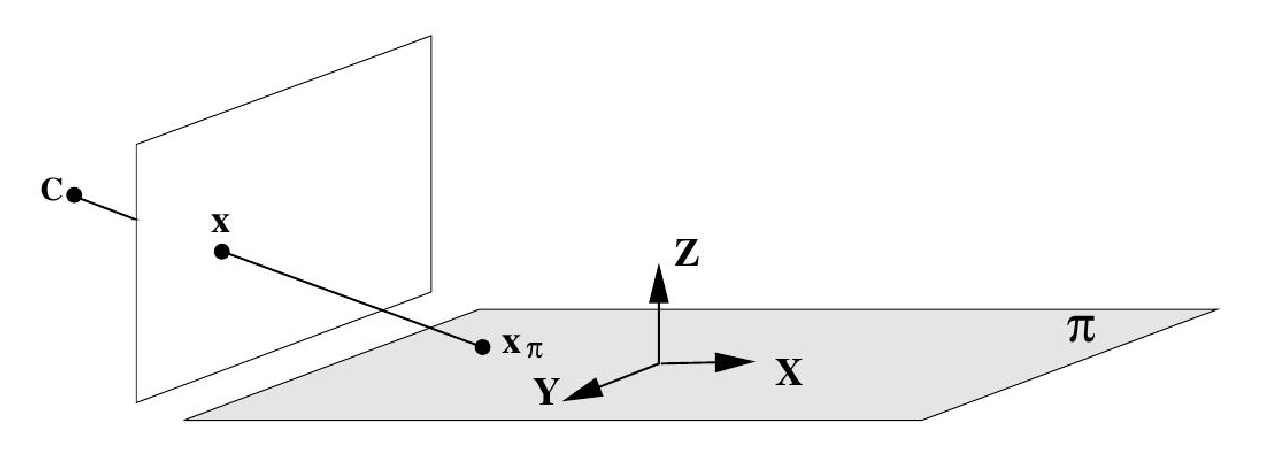
\includegraphics[scale=.5]{projecao-planos}}
\quad
\subfloat[]{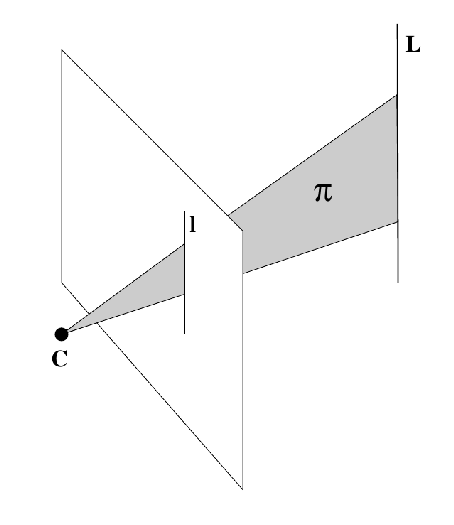
\includegraphics[scale=.5]{projecao-retas}}
\caption{({\tt a})\textit{Transformcao projetiva de plano a plano induzida pela camera $P$.}\,\,({\tt b})\textit{Plano $\bpi$ retroprojetado por uma reta $\lightrgb$ no plano da imagem atraves camera $P$.}}
\label{fig.projecao-planos-retas}
\end{figure}

\subsubsection{A ação projetiva de $P$ em retas.}\label{sec.proj.retas}
Geometricamente, como podemos ver na figura \ref{fig.projecao-planos-retas}, uma reta ${\bf L}$ no espaco 3D junto com o centro $\C$ da câmera definem um plano. A interseção desse plano com o plano da imagem é uma reta $\lightrgb$, que é a imagem da reta ${\bf L}$ no espaço. Algebricamente, considere uma reta ${\bf L}$ parametrizada por $\lambda$ passando pelos pontos ${\bf A}$ e ${\bf B}$, onde cada ponto nessa reta é dado por $\X(\lambda)={\bf A}+(\lambda)\,{\bf B}$. Considere ainda, ${\bf a}$ e ${\bf b}$ sendo as imagens dos pontos ${\bf A}$ e ${\bf B}$ sob a ação da câmera $P$. Aplicando a projeção da câmera $P$ aos pontos da reta ${\bf L}$ temos

\begin{equation*}
\begin{array}{rcl}
\x(\lambda)&=&P\,\X(\lambda)\\
&=&P({\bf A}+(\lambda)\,{\bf B})\\
&=&P\,{\bf A}+(\lambda)\,P\,{\bf B}\\
&=&{\bf a}+(\lambda)\,{\bf b},
\end{array}
\end{equation*}
onde cada $\x$ em função de $\lambda$ pertence à reta passando por ${\bf a}$ e ${\bf b}$ no plano da imagem.  

\subsubsection*{Retroprojeção de retas.}
Geometricamente, a retroprojeção de retas é o conjunto de pontos no espaço pertencentes a um plano, o qual é definido pelo centro da câmera e uma reta na imagem, como na figura \ref{fig.projecao-planos-retas}. Algebricamente, sendo a reta na imagem denotada por $\lightrgb$ e a camera por $P$, o plano retroprojetado é $P^\top\lightrgb$. De fato, um ponto $\X$ no espaco é projetado na imagem como $\x=P\,\X$, e esse ponto pertence a reta $\lightrgb$ na imagem se $\x^\top\lightrgb=0$ ou, substituindo, $(P\,\X)^\top\lightrgb=0$. Então, aplicando a transposta, $\X^\top P^\top\lightrgb=0$ e $P^\top\lightrgb$ é tomado como o plano que contém o ponto $\X$ no espaço. Assim, tal plano é retroprojetado da reta $\lightrgb$.  

\subsubsection{A ação projetiva de $P$ em cônicas.}
Um cone é uma quádrica degenerada, representada por uma matriz $4\times4$ que não tem posto completo, e é denotada por ${\tt Q}_{co}$.

\subsubsection*{Retroprojeção de cônicas.}
Uma cônica retroprojeta um cone ${\tt Q}_{co}$ que, neste caso, tem o vértice coincidindo com o centro da câmera, onde esse vértice é o vetor nulo da matriz $4\times4$ que representa o cone. Uma cônica retorpojeta um cone de acordo com 

\begin{equation*}
{\tt Q}_{co}=P^\top C\,P
\end{equation*}
pois, um ponto $\X$ no espaço é projetado na imagem na forma $\x=P\,\X$, e $\x\in C$ se satisfaz a equação $\x^\top C\,\x=0$. Substituindo $\x$ na equação da cônica temos $(P\,\X)^\top C\,P\,\X=0$, e aplicando a transposição, $\X^\top P^\top C\,P\,\X=0$. O ponto $\X$ é projetado na cônica $C$ se , se e somente se, $\X\in {\tt Q}_{co}$, que deve ser definida como ${\tt Q}_{co}=P^\top C\,P$. Assim, o cone é a retroprojeção da câmera. 

\subsubsection{A ação projetiva de $P$ em quádricas.}\label{sec.proj-quadricas}
Para tratarmos desse assunto, primeiramente precisamos definir alguns conceitos.

\subsubsection*{Contorno gerador e contorno aparente.}
Na formação da imagem de uma superfície, os raios de luz passando pelo centro da câmera são tangentes à essa superficie em 3D. O contorno dessa superfície nesses pontos de tangência é transformado num contorno no plano da imagem conforme a figura \ref{fig.cont-gerador-aparente}. O contorno da superfície é denominado \textit{contorno gerador} e denotado por ${\bf G}$, o contorno formado na imagem é chamado \textit{contorno aparente} e denotado por ${\bf g}$. Vale ressaltar que o contorno gerador depende das posições do centro da câmera e da própria superfície, e não depende do plano da imagem.  

\begin{figure}[htb!]
\centering
\subfloat[]{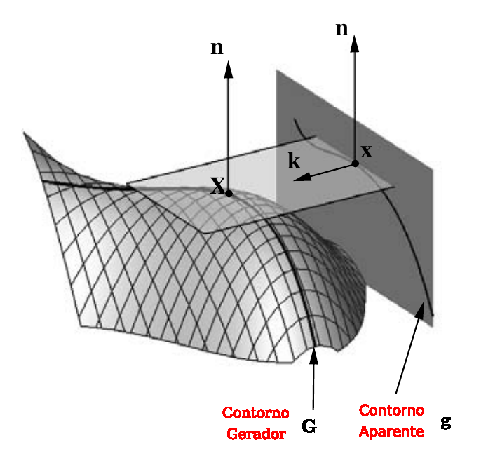
\includegraphics[scale=1.1]{contorno-gerador-aparente}}
\subfloat[]{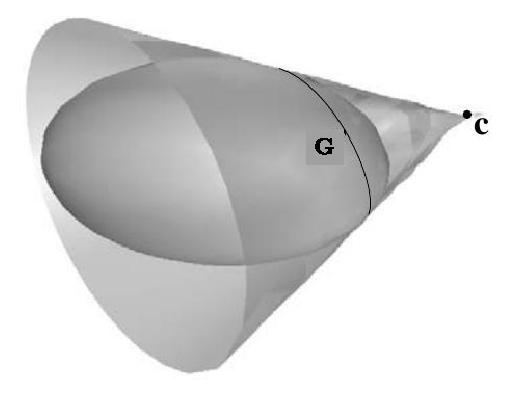
\includegraphics[scale=.95]{superficie-lisa}}
\caption{\textit{$({\tt a})\,$O contorno aparente é a imagem do contorno gerador, onde essa imagem fica definida pelas retas através do centro da câmera que são tangentes aos pontos no contorno gerador.$\,\,({\tt b})\,$}}
\label{fig.cont-gerador-aparente}
\end{figure}

\subsubsection*{Projeção de quádricas.}
A quádrica é uma superfície lisa  e o seu contorno gerador produz um contorno aparente no plano da imagem, através dos raios retroprojetados pelos pontos do contorno aparente e passando pelo centro da câmera, conforme um exemplo na figura \ref{fig.cont-gerador-aparente}. Assim, o contorno gerador é uma cônica e sob uma transformação projetiva o contorno aparente também é uma cônica na imagem. Como estamos usando relações de tangências aos contornos gerador e aparente, será necessária a utilização da quádrica dual	${\tt Q}^*$, já que esta define uma equação usando os planos que são tangentes ao contorno gerador. Seja $\lightrgb$ as retas tangentes à conica $C$ na imagem (contorno aparente), onde a cônica dual define a relação $\lightrgb^\top C^*\lightrgb=0$. Essas retas $\lightrgb$ retroprojetam planos definidos por $\bpi=P^\top\lightrgb$ (subseção \ref{sec.proj.retas}), que são tangentes à quádrica ${\tt Q}$ e satisfazem a relação $\bpi^\top {\tt Q}^*\bpi=0$. Substituindo o plano nessa última relação temos

\begin{equation*}
\begin{array}{rcl}
\bpi^\top {\tt Q}^*\bpi&=&(P^\top\lightrgb)^\top {\tt Q}^*P^\top\lightrgb\\
&=&\lightrgb^\top P\,{\tt Q}^*P^\top\lightrgb\\
&=&\lightrgb^\top C^*\lightrgb\\
&=&0,
\end{array}
\end{equation*}
onde tomamos $C^*=P\,{\tt Q}^*P^\top$, a imagem da quádrica sob a projeção $P$.

\subsection{A Geometria Bifocal}

\subsubsection{A Geometria Epipolar}

Considere um cenário com um ponto $\X$ no espaço 3D e dois planos que contêm as imagens desse ponto $\X$. Considere ainda um plano $\bpi$ que contém esse ponto $\X$ e os dois centros de projeção (ou centro da câmera) das duas câmeras, aqui denotados por $\C$ e $\C'$. A geometria epipolar se constitui nas relações existentes entre as interseções desse plano $\bpi$ com os dois planos das imagens observado na figura \ref{fig.geo-epipolar}. Sendo $\x$ a imagem 2D de $\X$ no primeiro plano de imagem, a construção desse cenário é motivada pela busca de $\x'$, também 2D, que seja correspondente a $\x$, onde $\x'$ é a imagem de $\X$ no segundo plano de imagem. Podemos observar que $\x$ e $\x'$ retroprojetam dois raios de luz definidos por $\C$ e $\C'$, onde esses raios pertencem a $\bpi$ e se intersectam em $\X$, e essa propriedade é essencial para nos auxiliar a definir as correspondências entre os pontos nas duas imagens. A \textit{reta base} é a reta que passa pelo centro de cada câmera $\C$ e $\C'$. O plano $\bpi$ fica determinado pela reta base e pelo raio de luz definido por $\x$ e $\C$, e a interseção de $\bpi$ com o segundo plano de imagem define uma reta chamada \textit{reta epipolar}, que é a imagem na segunda visão do raio de luz retroprojetado por $\x$. Ou seja, dadas duas imagens de uma cena, para cada ponto numa imagem vai existir uma reta epiplar correspondente na outra imagem. Pela construção, sabemos que $\x'\in\bpi$ e pertence ao plano da segunda imagem, portanto $\x'$ pertence à reta epipolar que será denotada por $\lightrgb'$. Assim, nossa busca pela correspondência de $\x$ se restringirá a uma busca numa reta e não a uma busca em todo o plano da segunda imagem. 

\begin{equation*}
\x\rightarrow\lightrgb'
\end{equation*}

Na geometria epipolar, a câmera que fotografar uma cena também deve fotografar a outra câmera, e a imagem do centro de projeção da primeira câmera na segunda visão é denominada \textit{epipolo} e denotada por $\e$. Analogamente, a imagem de $\C'$ na primeira visão também é chamada epipolo e é denotada por $\e'$.
O plano $\bpi$ é denominado \textit{plano epipolar} e num sistema com duas visões temos vários planos epipolares definidos por um único parâmetro, e que formam o feixe de planos girando em torno da reta base.

\begin{figure}[!htb]
\centering
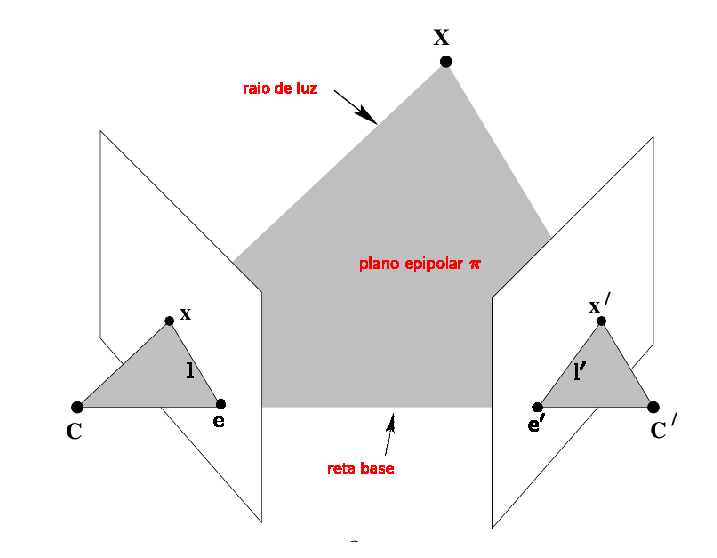
\includegraphics[scale=1.2]{geometria-epipolar}
\caption{\textit{O plano epipolar contém o ponto $\X$, os centros das câmeras, e define as retas epipolares em cada imagem, o que é a base para correspondência entre $\x$ e $\x'$.}}
\label{fig.geo-epipolar}
\end{figure}

\subsubsection{A Homografia Induzida por um Plano.}\label{sec.homografia}

Considere um plano $\bpi$ no espaco 3D com coordenadas expressas em um referencial no mundo, com duas visões, mas que não passa pelo centro de nenhuma das duas câmeras. Portanto esse plano não é o plano epipolar e é dito estar em posicões gerais. Assim, vamos determinar uma homografia definida em função desse plano $\bpi$.\\

Dadas as duas matrizes de projeção 

\begin{equation*}
P=[I|{\bf 0}]\qquad\text{e}\qquad P'=[R|{\bf t}],
\end{equation*}
(repare que as câmeras não são calibradas e a origem do sistema cartesiano do mundo coincide com o centro da primeira câmera) um plano $\bpi=({\bf v},1)^\top$, e um ponto $\X\in\bpi$, então a homografia induzida por $\bpi$ é

\begin{equation*}
\x'=H\,\x,\qquad\text{onde}\qquad H=R-{\bf t}\,{\bf v}^\top.
\end{equation*}

Podemos tomar a última coordenada de $\bpi$ igual a $1$ pois, por enquanto, nos interessa apenas que o plano não passe pelo centro da primeira câmera $\C=(0,0,0,1)^\top$. Observe o esquema na figura \ref{fig.homografia}. 

\begin{figure}[!htb]
\centering
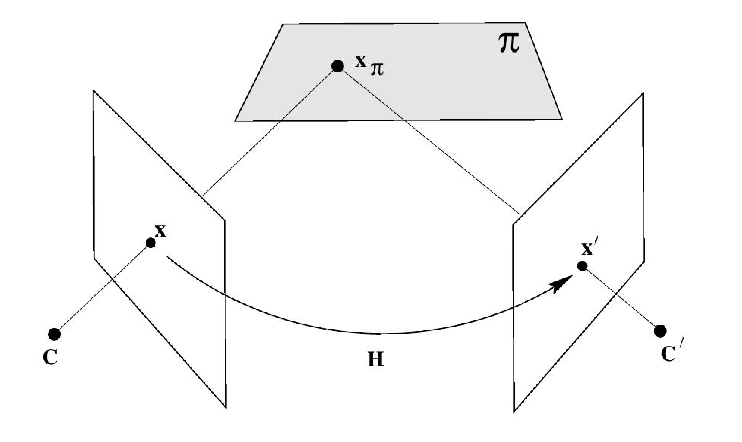
\includegraphics[scale=1.2]{homografia}
\caption{\textit{O mapeamento induzido por um plano no espaco 3D. O ponto $\x$ retroprojeta um raio que intersecta o plano $\bpi$ no ponto $\X_{\bpi}$, então $\X_{\bpi}$ é projetado na outra imagem em $\x'$.}}
\label{fig.homografia}
\end{figure}




Na primeira câmera temos a projeção

\begin{equation*}
\x=P\,\X=[I|{\bf 0}]\,\X,
\end{equation*}
e qualquer ponto 3D do tipo $\X=(\x^\top,\rho)^\top$ vai satisfazer a projeção acima. De fato

\begin{equation*}
P\,\X=
[I|{\bf 0}]\,(\x^\top,\rho)^\top=
\begin{bmatrix}
1&0&0&0\\
0&1&0&0\\
0&0&1&0
\end{bmatrix}
\begin{pmatrix}
x_1\\
x_2\\
x_3\\
\rho
\end{pmatrix}
=\x,
\end{equation*}
e assim qualquer ponto no raio de luz retroprojetado por $\x$ pode ser parametrizado por $\rho$. Como $\X\in\bpi$, $\bpi^\top\X=0$ e  
$\rho$ fica determinado

\begin{equation*}
\begin{array}{rcll}
\bpi^\top\,\X&=&0&\Rightarrow\\
({\bf v}^\top,1)\,(\x^\top,\rho)^\top&=&0&\Rightarrow\\
{\bf v}^\top\x+\rho&=&0&\Rightarrow\\
\rho&=&-{\bf v}^\top\,\x,&
\end{array}
\end{equation*}
e dessa forma o ponto $\X=(\x^\top,-{\bf v}^\top\x)^\top$.

Projetando o ponto 3D na segunda imagem temos

\begin{equation*}
\begin{array}{rcl}
\x'&=&P'\X\\
&=&[R|{\bf t}]\,(\x^\top,-{\bf v}^\top\x)^\top\\
&=&R\,\x-{\bf t}\,{\bf v}^\top\x\\
&=&(R-{\bf t}\,{\bf v}^\top)\,\x.
\end{array}
\end{equation*}
Portanto

\begin{equation*}
\x'=H\,\x,\qquad\text{onde}\qquad H=R-{\bf t}\,{\bf v}^\top.
\end{equation*}


\subsubsection{A Matriz Fundamental $F$}\label{sec.matriz-F}

A \textit{matriz fundamental} reúne todas as informações da geometria epipolar, é a representação algébrica dessa geometria de duas visões e, por isso, também é conhecida como \textit{tensor bifocal}. 

Geometricamente, a matriz fundamental pode ser obtida através do mapeamento de $\x$ na primeira imagem a um ponto $\x'$ na segunda imagem através de um plano $\bpi$ qualquer no espaço. Após esse mapeamento, identificamos a reta epipolar definida pelos pontos $\x'$ e $\e'$. Assim, considere um plano $\bpi$ que não passe pelos centros das câmeras, pois desse jeito um raio de luz retroprojetado por $\x$ deve intersectar o plano $\bpi$ em algum ponto $\X$. Usando a transferência através do plano $\bpi$, o ponto $\X$ deve ser projetado a um ponto $\x'$ na segunda imagem e, como $\X$ pertence ao raio retroprojetado por $\x$, o ponto $\x'$ deverá pertencer à reta epipolar $\lightrgb'$, já que $\lightrgb'$ é a imagem na segunda visão do raio retroprojetado por $\x$ conforme a figura \ref{fig.geo-epipolar}. Assim, pela subseção \ref{sec.homografia} existe uma homografia 2D $H$ em função de $\bpi$ onde cada ponto $\x_i$ é mapeado a um ponto $\x_i'$, 

\begin{equation}\label{eq.homo-plano}
\x'= H_{\bpi} \,\x,
\end{equation}
e eles são ditos projetivamente equivalentes, já que são projetivamente equivalentes a um mesmo ponto $\X_i$ no plano $\bpi$. Obtido o ponto $\x'$, a reta epipolar passando por $\x'$ e $\e'$ pode ser calculada fazendo 

\begin{equation}\label{eq.reta-epi-pro-vet}
\begin{array}{rcl}
\lightrgb'&=&\e'\times\x'\\
&=&[\e']_\times\x'
\end{array}
\end{equation}
($[\e']_\times$ está definida na subseção \ref{sec.anti-simetrica}). Substituindo \ref{eq.homo-plano} em \ref{eq.reta-epi-pro-vet} temos

\begin{equation*}
\begin{array}{rcl}
\lightrgb'&=&[\e']_\times\x'\\
&=&[\e']_\times H_{\bpi} \,\x\\
&=&F\,\x,
\end{array}
\end{equation*} 
onde definimos $F=[\e']_\times H_{\bpi}$ é a matriz fundamental. Como $[\e']_\times$ é uma matriz anti-simétrica $3\times3$ obtida de um vetor, então  $[\e']_\times$ tem posto $2$ e como $H_{\bpi}$ obtida de um plano tem posto $3$, temos que a matriz fundamental tem posto $2$. $F$ é o mapeamento de um plano projetivo a um feixe de retas epipolares.


Algebricamente, a matriz fundamental pode ser determinada à partir das matrizes das duas câmeras $P$ e $P'$. Vamos primeiramente definir a equação que representa o raio de luz retroprojetado por $\x$. Assim, dado um ponto $\x$ na imagem, precisamos determinar o conjunto de pontos no espaco 3D que são mapeados nesse ponto $\x$, e este raio (modelado por uma reta) será definido pela junção de dois de seus pontos. E conhecemos dois pontos pertencentes a este raio, $\C$ é o centro da câmera tal que $P\,\C=0$, e o ponto $P^+\x$ onde $P^+$ é a pseudo-inversa de $P$ definida na subseção \ref{sec.pseudo-P}. O ponto $P^+\x$ pertence ao raio pois aplicando-lhe a projeção efetuada pela câmera temos o próprio ponto $\x$ como retorno:

\begin{equation*}
P^+\x \rightarrow P\,P^+\x=I\,\x=\x.
\end{equation*}
Portanto, podemos formar o raio pela junção dos pontos $\C$ e $P^+\x$

\begin{equation*}
\X(\lambda)=P^+\x+\lambda\,\C.
\end{equation*}
Computando a imagem desses dois pontos na segunda visão temos

\begin{equation*}
\begin{array}{c}
P^+\x \rightarrow P'P^+\x\\
\C \rightarrow P'\C,
\end{array}
\end{equation*}
onde $P'\,\C$ é o epipolo na segunda imagem, e por isso, a reta epipolar pode ser definida em termos do produto vetorial desses dois pontos

\begin{equation*}
\lightrgb'=P'\C \times P'P^+\x.
\end{equation*}
Mas como $P'\C=\e'$, podemos substitui-lo na equação anterior

\begin{equation*}
\begin{array}{rcl}
\lightrgb'&=&P'\C \times P'P^+\x\\
&=&[\e']_\times P'P^+\x\\
&=&F\,\x,
\end{array}
\end{equation*}
definindo $F=[\e']_\times P'P^+$. Essa relação para $F$ é a mesma fórmula derivada anteriormente, com a homografia calculada em termos das duas câmeras, $H_{\bpi}=P'P^+$.


\subsection{Notação Usada por Fabbri}

Na seção anterior expusemos um tipo de notação bastante difundida na área de visão computacional mas que, por usar letras do nosso alfabeto, pode ocasionar alguma confusão ou mal entendido. Sendo assim, faz-se necessária a inclusão de uma nova notação que evite alguma ambiguidade e que favoreça a lucidez. Na tabela \ref{tab_not} temos um resumo da notação encontrada em \cite{Fabbri:Kimia:IJCV2015}, artigo o qual o leitor poderá consultar caso necessite de outras notações que não constam aqui. Essa nova notação é muito útil para a aplicação da projeção, já que para projetar um ponto na imagem fazemos a divisão de todas as três coordenadas desse ponto pela terceira coordenada. Outra ajuda acontece nas diferenciações, na obtenção das equações diferenciais e algébricas envolvidas no uso da geometria diferencial para abordar problemas do tipo. Nas abordagens feitas por hartley, usa-se correspondência de pontos e retas, basicamente, o que é feito pela maioria dos pesquisadores em visão computacional, e fica ruim para trabalhar com tangentes por conta dessa abordagem mais matricial. Com a notação apresentada aqui, as equações são explícitas e proporciona o emprego das tangentes.

\begin{table}[!h]
\begin{center}
\begin{tabular}{|c|l|}
\hline
Símbolos&Descrição\\\hline\hline
$\Gama^w$&Ponto 3D no sistema de coordenadas do mundo.\\\hline
$\Gama$&Ponto 3D no sistema de coordenadas da câmera.\\\hline
$\rot$&Matriz de rotação: coordenadas do mundo para a câmera.\\\hline
$\transl$&Vetor de translação.\\\hline
$\mathcal K$&Matriz de calibração: modelo basico (\textit{pinhole}).\\\hline
$\mathcal K_{im}$&Matriz de calibração: coordenadas do plano medidas em pixels.\\\hline
$\bc$&O centro da câmera.\\\hline
$\depth$&Profundidade do ponto imagem.\\\hline
$\gama$&Ponto 2D em coordenadas normalizadas.\\\hline
&Imagem da tangente a uma curva.\\\hline
$\T$&Tangente a uma curva no espaço: coordenadas da câmera.\\\hline
$\T^w$&Tangente a uma curva no espaço: coordenadas do mundo\\\hline
$K$&Curvatura.\\\hline
$G$&Velocidade de parametrizaçao.\\\hline
$\N^w$&Vetor normal.\\\hline
$\e_1$, $\e_2$, $\e_3$&Base de vetores do sistema de coordenadas da câmera.\\\hline
$\e_1^w$, $\e_2^w$, $\e_3^w$&Base de vetores do sistema de coordenadas do mundo.\\\hline
\end{tabular}
\end{center}
\caption{Notação.}
\label{tab_not}
\end{table}

Dada uma curva no espaço 3D conforme a figura \ref{curva_3D}, podemos fazer a representação de seus pontos nas coordenadas da câmera em função da representação dos mesmos pontos nas coordenadas do mundo de acordo com a relação:

\begin{figure}[!htb]
\centering
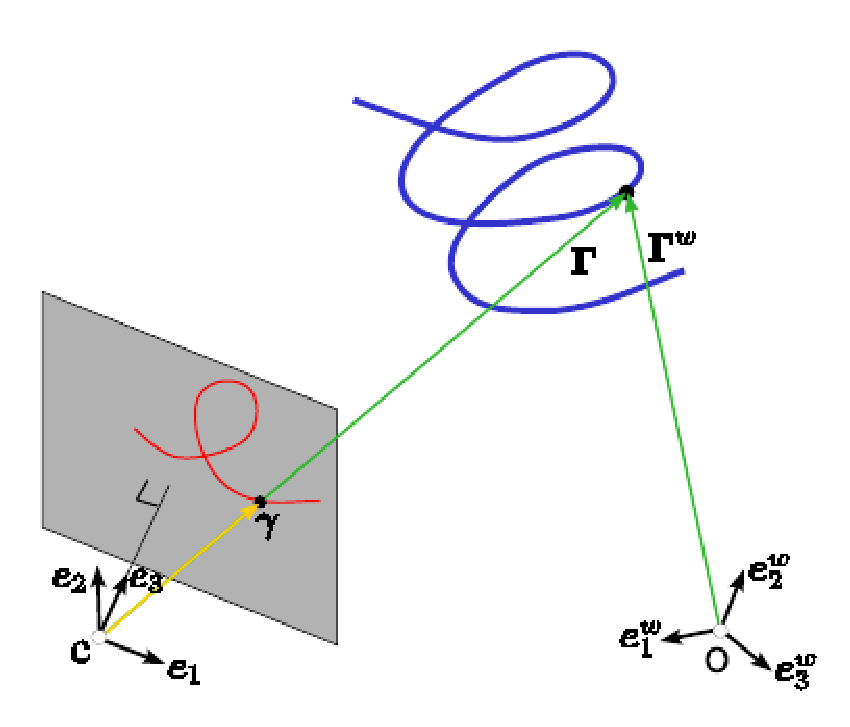
\includegraphics[scale=.8]{curva}
\caption{\textit{Cruva no espaço 3D e sua respectiva imagem 2D. Observe a representação de um mesmo ponto nas coordenadas do mundo e nas coordenadas da câmera.}}
\label{curva_3D}
\end{figure}


\begin{equation}\label{eq:coord:transf:RT}
\Gama = \rot (\Gama^w - \bc) \qquad \text{ou} \qquad \Gama = \rot\Gama^w + \transl,
\end{equation}
onde $\transl = -\rot\bc$ são as coordenadas da origem do espaço 3D expressas no sistema de coordenadas da câmera, e $\rot$ é a matriz de rotação.

A projeção de um ponto 3D $\Gama = [x,\, y,\, z]^\top$ no plano da imagem $z=1$ é o ponto $\gama = [\uu,\,\vv,\,1]^\top$ e esses pontos estão relacionados por:

\begin{equation}\label{eq:projection}[x,\, y,\, z]^\top =
[\depth\uu,\,\depth\vv,\,\depth]^\top \,\,\,\,\text{ou, compactamente,}\,\,\,\,  \Gama =
\depth\gama,
\end{equation}
onde $\depth$ é a profundidade extraída da terceira coordenada do vetor que representa o ponto 3D escrito nas coordenadas da câmera, $\depth = z = \e_3^\top\Gama$, e $\e_3^\top = [0,0,1]^\top$.

Substituindo $\depth$ em \ref{eq:projection} e isolando $\gama$, temos

\begin{align}
\gama &= \frac{\Gama}{\f^\top\Gama}.
\label{eq:projection:isolated:gamma}
\end{align}
e assim observamos que pontos na imagem são sempre tratados como um vetor 3D com $z=1$. 

Denotendo por $\gama^{(i)}$ a $i^{th}$ derivada de $\gama$ em relação a um parâmetro qualquer para $i$ um número natural, podemos verificar que

\begin{equation*}
\f^\top\gama^{(i)} = 0 \qquad \text{e} \qquad \f^\top\Gama^{(i)} = \depth^{(i)}.
\end{equation*}

Mais especificamente, calculando as derivadas primeira e segunda de $\depth$ obtemos

\begin{equation}\label{eq:depth:derivs}
\depth =
\e_3^\top\Gama,\qquad \depth' = G\e_3^\top\T,\qquad \depth'' = G'\e_3^\top\T +
G^2K\e_3^\top\N
\end{equation}
onde $G$ é a velocidade de parametrização, $\T^w$ é a tangente à curva no ponto $\Gama^{w}$ no espaço 3D, $K$ é a curvatura, e $\N^w$ é o vetor normal, cada qual com as seguintes definições:

\begin{equation}\label{eq:definicoes}
G  = \|\Gama^{w'}\|,\qquad \T^w = \frac{\Gama^{w'}}{G}, \qquad K  = \frac{\|\T^{w'}\|}{G} \qquad \text{e} \qquad \N^w = \frac{\T^{w'}}{\|\T^{w'}\|}.
\end{equation}

As definições da tangente e do vetor normal em \ref{eq:definicoes} foram dadas no sistema de coordenadas do mundo, enquanto em \ref{eq:depth:derivs} os mesmos são dados no sistema de coordenadas da câmera. Como visto anteriormente, para fazer a conversão basta aplicar 

\begin{equation*}
\T = \rot\T^w \qquad \text{e} \qquad \N = \rot\N^w,
\end{equation*}
e é interessante notar que para pontos perto/longe da curva temos $\depth' = 0$, $\e_3^\top\T = 0$.


Lembramos que a matriz de calibração para o modelo básico \textit{pinhole} é

\begin{center}
$
\begin{array}{cc}
\mathcal K = & \begin{bmatrix}
               f& &p_x\\
                &f&p_y\\
                & &1
               \end{bmatrix}, 
\end{array}
$
\end{center}
mas na prática, pontos na imagem são descritos em pixels, $\gama_{im} = [x_{im},\, y_{im},\, 1]^\top$ após a aplicação da matriz de calibração com os parâmetros internos 

\begin{equation}\label{eq:intrinsic:parameter:transf}
\gama_{im} = \mathcal K_{im}\gama,
\ \ \ \ \ \
\mathcal K_{im} = \begin{bmatrix}
\alpha_\uu & \sigma & \uu_o\\
0 &\alpha_\vv &  \vv_o\\
0 & 0 &  1
\end{bmatrix},
\end{equation}
onde $\uu_o$ e $\vv_o$ são as coordenadas do ponto principal na imagem, $\sigma$ define a inclinação entre os eixos cartesianos no plano da imagem (se $\sigma=0$ os eixos são perpendiculares), e
$\alpha_\uu$ e $\alpha_\vv$ são calculados dividindo-se a distância focal $f$ pela largura e altura do pixel medidas em unidades do mundo, respectivamente. Sendo $m_x$ e $m_y$ a largura e altura do pixel temos:

\begin{equation*}
\uu_o = \frac{p_x}{m_x}, \qquad \vv_o = \frac{p_y}{m_y}, \qquad \alpha_\uu = \frac{f}{m_x}, \qquad \alpha_\vv = \frac{f}{m_y}.
\end{equation*}



\subsection{Pesquisas Anteriores para Determinação de Câmera usando uma Imagem}

 O problema da determinação da pose de uma câmera  tem sido estudado extensivamente pela comunidade da área de visão computacional. Vamos citar alguns exemplos da determinação da pose de uma câmera.

\subsubsection{Usando três Pontos}
O caso mínimo da determinação de uma pose usando três pontos foi estudado por \cite{fischler}, e em seus estudos foi relatado o seguinte problema: 

``Dado um grupo de $m$ pontos de referência, cujas coordenadas 3D são conhecidas em um certo sistema de coordenadas, e dada uma imagem de um subconjunto desses $ m $ pontos de referência, determinar a localização (no sistema de coordenadas desses pontos de referência) do ponto onde a imagem foi registrada."

Assume-se que se conhece a correspondência entre os pontos de referência e os respectivos pontos na imagem, são conhecidos o ponto principal e o comprimento da distância focal para facilitar o cálculo dos ângulos entre pontos de referência a partir do centro da câmera, e por fim, assume-se que a câmera está localizada fora e ``acima" da região convexa formada pelos pontos de referência.
Desta forma, calculando as três distância entre o centro da câmera e  três pontos de referência (chamadas de ``pernas"), é possível determinar a posição da câmera bem como a orientação do plano da imagem. Nota-se que esses três pontos de referência formam um triângulo e, juntamente com o  centro da câmera, forma-se um tetraedro. Para calcular essas três ``pernas" pode-se aplicar a lei dos cossenos e formar um sistema com três equações. Em seguida, [10] explicita uma solução algébrica para o sistema bem como uma solução iterativa, calcula o centro da câmera e a orientação do plano da imagem.

Muitas outras formulações para problemas desse tipo foram comparadas e revisadas por \cite{haralick}. 

\subsubsection{Usando três Linhas}
 Para correspondência usando linha foi encontrada uma solução mínima usando três linhas e suas correspondências por \cite{chen}, como se segue:

Neste artigo não é determinada a pose de uma câmera, mas sim feita uma exposição para detrminação da localização de objetos em geral, com relação a um detrminiado sistema de coordendas. Sendo $\mathbf{m_i} $ a direção de uma linha $\mathbf{L_i} $ e $\mathbf{n_i} $ o vetor unitário normal a um plano $\mathbf{F_i} $. Além disso, $\mathbf{p_i} $ é a posição de um ponto na linha $\mathbf{L_i} $ e $\mathbf{d_i} $ é a distância entre $\mathbf{F_i} $ e a origem do sistema de coordenadas. O problema pode ser matematicamente formulado:
Dados $\mathbf{m_i} $,$\mathbf{n_i} $,$\mathbf{p_i} $,$\mathbf{d_i} $, determinar $ R $ e $ \mathbf{t} $ de maneira que 
\begin{equation*}
{\bf n}_i^{T}\,R\,{\bf m}_i = 0 \qquad {\bf n}_i^T\,(R\,{\bf p}_i+{\bf t}) = {\bf d}_i
\end{equation*}

As equações significam que, para uma matriz de rotação, o vetor linha rotacionado é perpendicular ao vetor normal. E, para um vetor de translação, o ponto transladado perntencerá ao plano. Mais ainda, toda a linha que contém esse ponto estará contida no plano. Como são necessárias seis restrições para a matriz de rotação e o vetor de translação, precisa-se de pelo menos três pares de correspondência para resolver o problema, pois cada par nos fornece duas equações.

A solução dada por \cite{chen} é chamada solução canônica e consiste basicamente em calcular a matriz de rotação usando a primeira relação, definindo essa matriz com uma multiplicação de outras três matriz de rotação, onde cada uma produz uma rotação em torno de um eixo, os quais formam entre si uma base perpendicular. A primeira relação gera um sistema com duas equações onde é dada uma solução numérica. As entradas do vetor de translação são lineares na segunda relação, e são calculadas após o cálculo da matriz de rotação, usando um sistema com três equações.

Outro desenvolvimento envolvendo linhas pode ser encontrado em \cite{dhome}.

\subsubsection{Usando Combinação de Pontos e Linhas}
Recentemente, um caso mínimo usando combinação de pontos e linhas foi publicado \cite{ramalingam}. Na correspondência entre pontos, usa-se o fato de que os pontos  ${\bf X}$ 3D na cena, ${\bf x}$ 2D na imagem e ${\bf C}$ o centro da câmera, estão alinhados. Esses pontos são empilhados numa matriz $3\times4$, onde cada submatriz $3\times3$ terá determinante zero por conta da linearidade dos pontos. As entradas do ponto 2D imagem nessa matriz são colocadas em função da matriz de rotação $R$ e do vetor de translação ${\bf t}$, retirados da equação de projeção $\lambda\,{\bf x}={\bf P}\,{\bf X}$.

\begin{center}
$\begin{bmatrix}
C_1 & X_1 & R_{1,1}\,X_1\,+\,R_{1,2}\,X_2\,+\,R_{1,3}\,X_3\,+\,t_1 \\ 
C_2 & X_2 & R_{2,1}\,X_1\,+\,R_{2,2}\,X_2\,+\,R_{2,3}\,X_3\,+\,t_2 \\ 
C_3 & X_3 & R_{3,1}\,X_1\,+\,R_{3,2}\,X_2\,+\,R_{3,3}\,X_3\,+\,t_3 \\ 
1 & 1 & 1
\end{bmatrix} $
\end{center}

Apesar do cálculo de quatro derterminantes na matriz acima, temos apenas duas restrições já que nem todas as equações são L.I.

Uma abordagem similar é construída para as correspondências entre linhas. Uma linha na cena possui pontos extremos ${\bf X}_1$ e ${\bf X}_2$, a linha correspondente na imagem possui extremos ${\bf x}_1$ e ${\bf x}_2$. Esses quatro pontos saõ coplanares juntamente com o centro ${\bf C}$ da câmera e, por isso, o determinante da matriz abaixo deve ser zero.

\begin{center}
$\begin{bmatrix}
C_x & X_{1,x} & X_{2,x} & R_{1,1}\,X_{1,x}\,+\,R_{1,2}\,X_{1,y}\,+\,R_{1,3}\,X_{1,z}\,+\,t_1 \\ 
C_y & X_{1,y} & X_{2,y} & R_{2,1}\,X_{2,x}\,+\,R_{2,2}\,X_{2,y}\,+\,R_{2,3}\,X_{2,z}\,+\,t_2 \\ 
C_z & X_{1,z} & X_{2,z} & R_{3,1}\,X_{3,x}\,+\,R_{3,2}\,X_{3,y}\,+\,R_{3,3}\,X_{3,z}\,+\,t_3 \\ 
1 & 1 & 1 & 1
\end{bmatrix} $
\end{center}

O determinante dessa matriz fornece uma restrição usando a imagem ${\bf x}_1$, mas consegue-se outra restrição com o determinante de uma matriz similar usando a imagem ${\bf x}_2$. Assim, combinando duas linhas e um ponto ou dois pontos e uma linha, obtém-se as seis restrições necessárias. Com uma mudança de coordenadas que satisfaz algumas condições, ficam determinados os pontos na imagem, na cena e o centro da câmera. Além disso, o sistema de equações fica reduzido a um polinômino de grau 4 a 8, bem menor que o original (antes da mudança de coordenadas) que era 64. Outro estudo bastante interessante usando combinações de pontos, linhas e tagentes  pode ser encontrado em \cite{bib:kuang}. Nesse estudo, observa-se ainda a aplicação de técnicas recentes de resolução de sistemas de equações polinomiais multivariadas, baseadas em geometria algébrica. 

\subsubsection{Usando quatro Pontos não Coplanares}
A generalização para casos não planares, o caso mínimo usando quatro pontos 2D-3D foi primeiramente resolvido por \cite{triggs}. A ideia basica é determinar a pose e a distancia focal usando quatro correspondencias e tomando a matriz de calibraçao com os valores padronizados:

\begin{center}
$\begin{array}{cc}
K =  & \begin{bmatrix}
 0 & 0 & 0 \\ 
 0 & 1 & 0 \\ 
 0 & 0 & 1/f
\end{bmatrix} 
\end{array}$
\end{center}

O primeiro passo é parecido com o algoritmo DLT onde dado um ponto 3D e sua imagem $\lambda\,{\bf x} = P\,{\bf X}$, elimina-se a profundidade $\lambda$ com o produto cruzado ${\bf x}\times P\,{\bf X} = {\bf 0}$ e escolhe-se duas restrições em $P$. Transformando ${\bf x}$ numa matriz de \textit{Householder}, as restrições podem ser reunidas numa matriz $2\,n\times 12$, e no caso do uso de quatro pontos teremos uma matriz $8\times 12$ que tem posto $8$ e deixa $4$ espaços nulos. $P$ pode ser descrita como:

\begin{center}
$P = P(\mu)\equiv\sum_{i=1}^d{\mu_i\,P_i} $,
\end{center}

onde $P_i$ são as matrizes $3\times 4$ correspondentes a cada vetor base do espaço nulo, os quais são calculados numericamente através da decomposição SVD.

Sendo a decomposição $P\simeq K\,R(I| -{\bf t})$, a matriz quádrica absoluta e sua imagem

\begin{center}$
\begin{array}{cc}
\begin{array}{cc}
\Omega \equiv  & \begin{bmatrix}
1 & 0 & 0 & 0 \\ 
0 & 1 & 0 & 0 \\ 
0 & 0 & 1 & 0 \\ 
0 & 0 & 0 & 0
\end{bmatrix} 
\end{array} 
 & \text{e} \quad \omega \equiv P\,\Omega P^{T} \simeq KK^{T} \text{, respectivamente.}
\end{array}$ 
\end{center}

Assim pode-se converter as restrições em $K$ naquelas das candidatas $P(\mu)$ ou nas imagens $\omega$:

\begin{center}
$\omega  = \omega (\mu) \equiv P(\mu)\,\Omega P(\mu)^T$
\end{center}  

Como $K = diag((f,f,1)$ então $K\,K^T = diag(f^2,f^2,1)$ e, consequentemente, 
\begin{center}
$\omega _{1,1} = \omega_{2,2}$ \quad e \quad $\omega_{1,2} = \omega_{1,3} = \omega_{2,3} = 0$
\end{center}

Assim temos um sistema de equações quadráticas nas quatro variáveis $\mu_i$ que tem pelo menos uma solução. Pode-se usar a decomposição SVD para obter os $\mu_i$, sustituí-los em $P(\mu)$ para obter $P$, em seguida fazer a decomposição de $P$ para obter pose e calibração. A matriz resultante é grande, $80\times 56$ mas ainda sim é tratável.


 Outros autores como \cite{bujnak} resoveram para um caso mínimo de quatro pontos para câmeras sem conheciemnto da distância focal e distorção radial.

\subsubsection{Usando Pontos-Tangentes}
Em \cite{Fabbri:Giblin:Kimia:ECCV12} uma solução é dada usando um problema mínimo de dois pontos-tangentes,$\lbrace ({\bf X}_1^w,{\bf T}_1^w),({\bf X}_2^w,{\bf T}_2^w)\rbrace$, e suas respectivas imagens $\lbrace ({\bf x}_1,{\bf t}_1),({\bf x}_2,{\bf t}_2)\rbrace$. No artigo é demonstrado que a solução pode ser obtida resolvendo um sistema com duas equações:

\begin{center}
$\begin{cases}
{\bf x}_1^T\,{\bf x}_1\,\rho_1^2 - 2\,{\bf x}_1^T\,{\bf x}_2\,\rho_1\,\rho_2 + {\bf x}_2^T\,{\bf x}_2\,\rho_2^2 = ||{\bf X}_1^w - {\bf X}_2^w||\\
Q(\rho_1,\rho_2) = 0,
\end{cases}$
\end{center}

onde $\rho$ é a profundidade em ${\bf x} = \rho\,{\bf X}$, $Q$ é um polinômio de grau 8, e a pose da câmera $R, {\bf \tau}$ relativa ao sistema de coordenadas do mundo é definida por ${\bf X} = R\,{\bf X}^w  + \tau$. 

Fazendo-se umas substituições e isolando $R\, \text{e}\, \tau$ temos:

\begin{center}
$\begin{cases}
R = [({\bf X}_1^w - {\bf X}_2^w)\,{\bf T}_1^w\,{\bf T}_2^w]^{-1} \cdot [\rho_1\,{\bf x}_1 - \rho_2\,{\bf x}_2\,\rho_1\,\frac{g_1}{G_1}\,{\bf t}_1 + \frac{\rho_1'}{G_1}\,{\bf x}_1\,\rho_2\,\frac{g_2}{G_2}\,{\bf t}_2 + \frac{\rho_2'}{G_2}\,{\bf x_2}]\\
\tau = \rho_1\,{\bf x}_1 - R\,{\bf X}_1^w.
\end{cases}$
\end{center}

Em material suplementar estão disponíveis expressões para $\frac{g_1}{G_1}, \frac{g_2}{G_2}\text{(razão das velocidades)}, \rho_1 \,\text{e}\, \rho_2$. 


\subsection{Resumo dos Resultados Fabbri}
Projeção e reconstrução 3D com o uso de tangentes.


%\section{Pesquisas Anteriores para a Determinação de Pose}
 
 O problema da determinação da pose de uma câmera  tem sido estudado extensivamente pela comunidade da área de visão computacional. Vamos citar alguns exemplos da determinação da pose de uma câmera.

\subsection{Usando três Pontos}
O caso mínimo da determinação de uma pose usando três pontos foi estudado por \cite{fischler}, e em seus estudos foi relatado o seguinte problema: 

``Dado um grupo de $m$ pontos de referência, cujas coordenadas 3D são conhecidas em um certo sistema de coordenadas, e dada uma imagem de um subconjunto desses $ m $ pontos de referência, determinar a localização (no sistema de coordenadas desses pontos de referência) do ponto onde a imagem foi registrada."

Assume-se que se conhece a correspondência entre os pontos de referência e os respectivos pontos na imagem, são conhecidos o ponto principal e o comprimento da distância focal para facilitar o cálculo dos ângulos entre pontos de referência a partir do centro da câmera, e por fim, assume-se que a câmera está localizada fora e ``acima" da região convexa formada pelos pontos de referência.
Desta forma, calculando as três distância entre o centro da câmera e  três pontos de referência (chamadas de ``pernas"), é possível determinar a posição da câmera bem como a orientação do plano da imagem. Nota-se que esses três pontos de referência formam um triângulo e, juntamente com o  centro da câmera, forma-se um tetraedro. Para calcular essas três ``pernas" pode-se aplicar a lei dos cossenos e formar um sistema com três equações. Em seguida, [10] explicita uma solução algébrica para o sistema bem como uma solução iterativa, calcula o centro da câmera e a orientação do plano da imagem.

Muitas outras formulações para problemas desse tipo foram comparadas e revisadas por \cite{haralick}. 

\subsection{Usando três Linhas}
 Para correspondência usando linha foi encontrada uma solução mínima usando três linhas e suas correspondências por \cite{chen}, como se segue:

Neste artigo não é determinada a pose de uma câmera, mas sim feita uma exposição para detrminação da localização de objetos em geral, com relação a um detrminiado sistema de coordendas. Sendo $\mathbf{m_i} $ a direção de uma linha $\mathbf{L_i} $ e $\mathbf{n_i} $ o vetor unitário normal a um plano $\mathbf{F_i} $. Além disso, $\mathbf{p_i} $ é a posição de um ponto na linha $\mathbf{L_i} $ e $\mathbf{d_i} $ é a distância entre $\mathbf{F_i} $ e a origem do sistema de coordenadas. O problema pode ser matematicamente formulado:
Dados $\mathbf{m_i} $,$\mathbf{n_i} $,$\mathbf{p_i} $,$\mathbf{d_i} $, determinar $ R $ e $ \mathbf{t} $ de maneira que 
\begin{equation*}
{\bf n}_i^{T}\,R\,{\bf m}_i = 0 \qquad {\bf n}_i^T\,(R\,{\bf p}_i+{\bf t}) = {\bf d}_i
\end{equation*}

As equações significam que, para uma matriz de rotação, o vetor linha rotacionado é perpendicular ao vetor normal. E, para um vetor de translação, o ponto transladado perntencerá ao plano. Mais ainda, toda a linha que contém esse ponto estará contida no plano. Como são necessárias seis restrições para a matriz de rotação e o vetor de translação, precisa-se de pelo menos três pares de correspondência para resolver o problema, pois cada par nos fornece duas equações.

A solução dada por \cite{chen} é chamada solução canônica e consiste basicamente em calcular a matriz de rotação usando a primeira relação, definindo essa matriz com uma multiplicação de outras três matriz de rotação, onde cada uma produz uma rotação em torno de um eixo, os quais formam entre si uma base perpendicular. A primeira relação gera um sistema com duas equações onde é dada uma solução numérica. As entradas do vetor de translação são lineares na segunda relação, e são calculadas após o cálculo da matriz de rotação, usando um sistema com três equações.

Outro desenvolvimento envolvendo linhas pode ser encontrado em \cite{dhome}.

\subsection{Usando Combinação de Pontos e Linhas}
Recentemente, um caso mínimo usando combinação de pontos e linhas foi publicado \cite{ramalingam}. Na correspondência entre pontos, usa-se o fato de que os pontos  ${\bf X}$ 3D na cena, ${\bf x}$ 2D na imagem e ${\bf C}$ o centro da câmera, estão alinhados. Esses pontos são empilhados numa matriz $3\times4$, onde cada submatriz $3\times3$ terá determinante zero por conta da linearidade dos pontos. As entradas do ponto 2D imagem nessa matriz são colocadas em função da matriz de rotação $R$ e do vetor de translação ${\bf t}$, retirados da equação de projeção $\lambda\,{\bf x}={\bf P}\,{\bf X}$.

\begin{center}
$\begin{bmatrix}
C_1 & X_1 & R_{1,1}\,X_1\,+\,R_{1,2}\,X_2\,+\,R_{1,3}\,X_3\,+\,t_1 \\ 
C_2 & X_2 & R_{2,1}\,X_1\,+\,R_{2,2}\,X_2\,+\,R_{2,3}\,X_3\,+\,t_2 \\ 
C_3 & X_3 & R_{3,1}\,X_1\,+\,R_{3,2}\,X_2\,+\,R_{3,3}\,X_3\,+\,t_3 \\ 
1 & 1 & 1
\end{bmatrix} $
\end{center}

Apesar do cálculo de quatro derterminantes na matriz acima, temos apenas duas restrições já que nem todas as equações são L.I.

Uma abordagem similar é construída para as correspondências entre linhas. Uma linha na cena possui pontos extremos ${\bf X}_1$ e ${\bf X}_2$, a linha correspondente na imagem possui extremos ${\bf x}_1$ e ${\bf x}_2$. Esses quatro pontos saõ coplanares juntamente com o centro ${\bf C}$ da câmera e, por isso, o determinante da matriz abaixo deve ser zero.

\begin{center}
$\begin{bmatrix}
C_x & X_{1,x} & X_{2,x} & R_{1,1}\,X_{1,x}\,+\,R_{1,2}\,X_{1,y}\,+\,R_{1,3}\,X_{1,z}\,+\,t_1 \\ 
C_y & X_{1,y} & X_{2,y} & R_{2,1}\,X_{2,x}\,+\,R_{2,2}\,X_{2,y}\,+\,R_{2,3}\,X_{2,z}\,+\,t_2 \\ 
C_z & X_{1,z} & X_{2,z} & R_{3,1}\,X_{3,x}\,+\,R_{3,2}\,X_{3,y}\,+\,R_{3,3}\,X_{3,z}\,+\,t_3 \\ 
1 & 1 & 1 & 1
\end{bmatrix} $
\end{center}

O determinante dessa matriz fornece uma restrição usando a imagem ${\bf x}_1$, mas consegue-se outra restrição com o determinante de uma matriz similar usando a imagem ${\bf x}_2$. Assim, combinando duas linhas e um ponto ou dois pontos e uma linha, obtém-se as seis restrições necessárias. Com uma mudança de coordenadas que satisfaz algumas condições, ficam determinados os pontos na imagem, na cena e o centro da câmera. Além disso, o sistema de equações fica reduzido a um polinômino de grau 4 a 8, bem menor que o original (antes da mudança de coordenadas) que era 64. Outro estudo bastante interessante usando combinações de pontos, linhas e tagentes  pode ser encontrado em \cite{bib:kuang}. Nesse estudo, observa-se ainda a aplicação de técnicas recentes de resolução de sistemas de equações polinomiais multivariadas, baseadas em geometria algébrica. 

\subsection{Usando quatro Pontos não Coplanares}
A generalização para casos não planares, o caso mínimo usando quatro pontos 2D-3D foi primeiramente resolvido por \cite{triggs}. A ideia basica é determinar a pose e a distancia focal usando quatro correspondencias e tomando a matriz de calibraçao com os valores padronizados:

\begin{center}
$\begin{array}{cc}
K =  & \begin{bmatrix}
 0 & 0 & 0 \\ 
 0 & 1 & 0 \\ 
 0 & 0 & 1/f
\end{bmatrix} 
\end{array}$
\end{center}

O primeiro passo é parecido com o algoritmo DLT onde dado um ponto 3D e sua imagem $\lambda\,{\bf x} = P\,{\bf X}$, elimina-se a profundidade $\lambda$ com o produto cruzado ${\bf x}\times P\,{\bf X} = {\bf 0}$ e escolhe-se duas restrições em $P$. Transformando ${\bf x}$ numa matriz de \textit{Householder}, as restrições podem ser reunidas numa matriz $2\,n\times 12$, e no caso do uso de quatro pontos teremos uma matriz $8\times 12$ que tem posto $8$ e deixa $4$ espaços nulos. $P$ pode ser descrita como:

\begin{center}
$P = P(\mu)\equiv\sum_{i=1}^d{\mu_i\,P_i} $,
\end{center}

onde $P_i$ são as matrizes $3\times 4$ correspondentes a cada vetor base do espaço nulo, os quais são calculados numericamente através da decomposição SVD.

Sendo a decomposição $P\simeq K\,R(I| -{\bf t})$, a matriz quádrica absoluta e sua imagem

\begin{center}$
\begin{array}{cc}
\begin{array}{cc}
\Omega \equiv  & \begin{bmatrix}
1 & 0 & 0 & 0 \\ 
0 & 1 & 0 & 0 \\ 
0 & 0 & 1 & 0 \\ 
0 & 0 & 0 & 0
\end{bmatrix} 
\end{array} 
 & \text{e} \quad \omega \equiv P\,\Omega P^{T} \simeq KK^{T} \text{, respectivamente.}
\end{array}$ 
\end{center}

Assim pode-se converter as restrições em $K$ naquelas das candidatas $P(\mu)$ ou nas imagens $\omega$:

\begin{center}
$\omega  = \omega (\mu) \equiv P(\mu)\,\Omega P(\mu)^T$
\end{center}  

Como $K = diag((f,f,1)$ então $K\,K^T = diag(f^2,f^2,1)$ e, consequentemente, 
\begin{center}
$\omega _{1,1} = \omega_{2,2}$ \quad e \quad $\omega_{1,2} = \omega_{1,3} = \omega_{2,3} = 0$
\end{center}

Assim temos um sistema de equações quadráticas nas quatro variáveis $\mu_i$ que tem pelo menos uma solução. Pode-se usar a decomposição SVD para obter os $\mu_i$, sustituí-los em $P(\mu)$ para obter $P$, em seguida fazer a decomposição de $P$ para obter pose e calibração. A matriz resultante é grande, $80\times 56$ mas ainda sim é tratável.


 Outros autores como \cite{bujnak} resoveram para um caso mínimo de quatro pontos para câmeras sem conheciemnto da distância focal e distorção radial.

\subsection{Usando Pontos-Tangentes}
Em \cite{Fabbri:Giblin:Kimia:ECCV12} uma solução é dada usando um problema mínimo de dois pontos-tangentes,$\lbrace ({\bf X}_1^w,{\bf T}_1^w),({\bf X}_2^w,{\bf T}_2^w)\rbrace$, e suas respectivas imagens $\lbrace ({\bf x}_1,{\bf t}_1),({\bf x}_2,{\bf t}_2)\rbrace$. No artigo é demonstrado que a solução pode ser obtida resolvendo um sistema com duas equações:

\begin{center}
$\begin{cases}
{\bf x}_1^T\,{\bf x}_1\,\rho_1^2 - 2\,{\bf x}_1^T\,{\bf x}_2\,\rho_1\,\rho_2 + {\bf x}_2^T\,{\bf x}_2\,\rho_2^2 = ||{\bf X}_1^w - {\bf X}_2^w||\\
Q(\rho_1,\rho_2) = 0,
\end{cases}$
\end{center}

onde $\rho$ é a profundidade em ${\bf x} = \rho\,{\bf X}$, $Q$ é um polinômio de grau 8, e a pose da câmera $R, {\bf \tau}$ relativa ao sistema de coordenadas do mundo é definida por ${\bf X} = R\,{\bf X}^w  + \tau$. 

Fazendo-se umas substituições e isolando $R\, \text{e}\, \tau$ temos:

\begin{center}
$\begin{cases}
R = [({\bf X}_1^w - {\bf X}_2^w)\,{\bf T}_1^w\,{\bf T}_2^w]^{-1} \cdot [\rho_1\,{\bf x}_1 - \rho_2\,{\bf x}_2\,\rho_1\,\frac{g_1}{G_1}\,{\bf t}_1 + \frac{\rho_1'}{G_1}\,{\bf x}_1\,\rho_2\,\frac{g_2}{G_2}\,{\bf t}_2 + \frac{\rho_2'}{G_2}\,{\bf x_2}]\\
\tau = \rho_1\,{\bf x}_1 - R\,{\bf X}_1^w.
\end{cases}$
\end{center}

Em material suplementar estão disponíveis expressões para $\frac{g_1}{G_1}, \frac{g_2}{G_2}\text{(razão das velocidades)}, \rho_1 \,\text{e}\, \rho_2$. 

\texttt{ correspondência necessária é reduzida a uma única correspondência local feita por [20 - koser,koch].Contudo, esta última configuração é muito sensível aos ruídos medidos na correspondência. Para determinação de pose de câmera sem conhecimento da distância focal, o caso com imagens no mesmo plano foi formulado por [1 - abidi,chandra].  Soluções eficientes  e numericamente estáveis foram desenvolvidas por [4 - bujnak et.al.]. Combinando correspondências 2D-2D e 2D-3D, [19 - josephson, astrom, et. al.] investigaram muitos casos mínimos para determinação da pose sem conhecimento da distância focal.   }


\newpage
\section{Geometria trifocal}\label{sec.geo-tri}
Assim como num sistema com duas imagens, podemos extrair informações sobre o cenário em 3D através da correspondência entre pontos, retas, tangentes e segmentos de curvas com três  ou mais imagens. No entanto, grande parte das pesquisas em visão computacional não tem utilizado a geometria trifocal em problemas de reconstrução 3D e transferência de pontos de uma imagem para outra. Menor ainda é a utilização da geometria diferencial para abordar esses problemas para curvas gerais, tais como cristas de ondas. Um dos nossos objetivos é fazer um levantamento das características e conceitos encontrados num sistema trifocal em comparação com a geometria epipolar, e relatar alguns dos benefícios conseguidos através da inclusão de uma terceira imagem.

\subsection{O Problema}
Considere um cenário em 3D com três imagens em 2D desse cenário. Nessas três imagens, temos as correspondências entre pontos, onde esses pontos correpondentes $\x\leftrightarrow\x'\leftrightarrow\x''$ (dois sinais de apóstrofo indicam o objeto pertencente à terceira câmera) previamente conhecidos, são três imagens de um mesmo ponto desconhecido $\X$ em 3D. O desafio da reconstrução 3D é determinar, a partir das correspondências nas imagens, as matrizes das câmeras $P$, $P'$ e $P''$ que realizam as projeções $\x=P\,\X$, $\x'=P'\X$ e $\x''=P''\X$ em cada imagem, bem como a determinação do ponto $\X$. Nesse trabalho será dada prioridade para determinação das matrizes das câmeras por ser um dos maiores problemas atuais em visão computacional. 

É mais comum a utilização da geometria epipolar para problemas de reconstrução 3D, fazendo a extração das câmeras usando a geometria epipolar e aplicando um algoritmo para determinação do ponto 3D a partir da triangulação $(\x,\x',\X)$. Mas quando aumentamos para três a quantidade de imagens, aumenta-se também as possibilidades de degenerações (que depende  da posição do ponto 3D $\X$) se continuarmos utilizando as ferramentas da geometria epipolar. Mostraremos que alguns casos de degenerações podem ser removidos usando a teoria da geometria trifocal.
Vamos aplicar o procedimento contido em \citep{Faugeras} que consiste em utilizar a matriz fundamental e a geometria epipolar num problema de transferência de pontos num sistema trifocal, avaliar as deficiências dessa abordagem e em seguida mostrar como a geometria trifocal pode erradicar algumas dessas deficiências. 

Considere a figura \ref{fig.trifocal-frente} onde podemos visualizar as três imagens $\x$, $\x'$ e $\x''$ de um ponto 3D $\X$. 

\begin{figure}
\centering
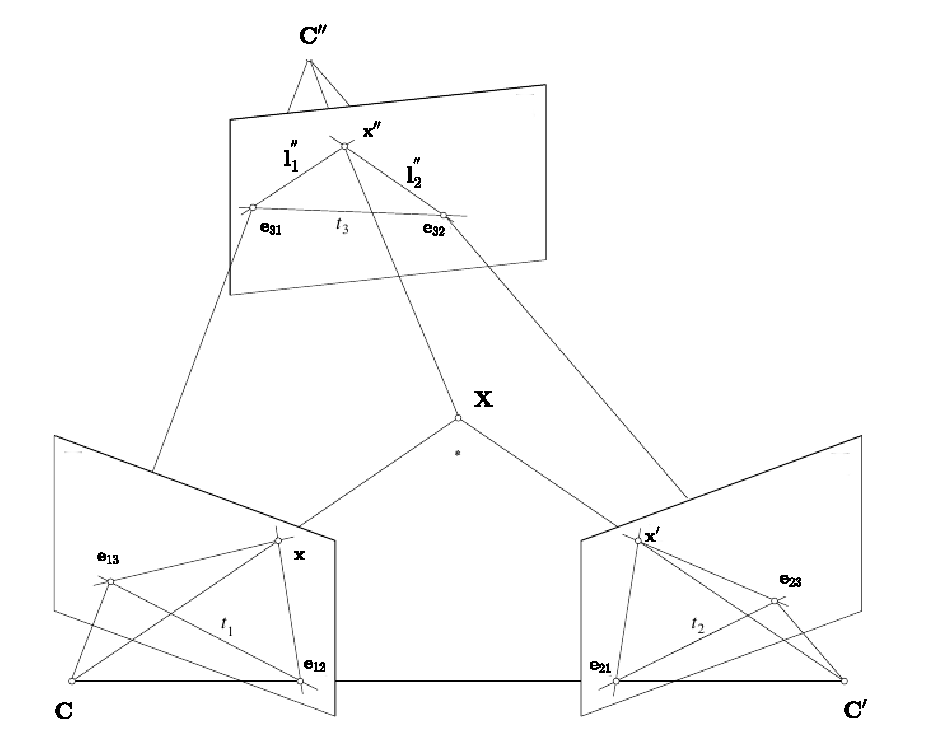
\includegraphics[scale=.8]{trifocal-frente-frente}
\caption{{\it O plano trifocal juntamente com os três planos epipolares. A transferência epipolar falha em alguns casos.}}
\label{fig.trifocal-frente}
\end{figure}

O plano definido pelos pontos $\C, \C' \,\,\text{e}\,\, \X$ forma o plano epipolar para as câmeras 1 e 2. Analogamente, temos o plano epipolar para as câmeras 1 e 3 e para as câmeras 2 e 3. A interseção de cada plano epipolar com os planos das imagens geram as retas epipolares. Por exemplo, a reta  epipolar $\lightrgb''_1$ definida pelos pontos $\e_{31}$ e $\x''$ na terceira imagem, é a reta epipolar com relação ao ponto $\x$ na primeira imagem. Ou seja, $\lightrgb''_1$ é a imagem, na câmera 3, da reta retroprojetada por $\x$ através do centro de projeção $\C$ na câmera 1. Essa reta é definida por $\lightrgb''_1=F_{31}\,\x$ ou $\lightrgb''_1=\e_{31}\times\x''$, onde $F_{ij}$ é a matriz fundamental para as câmeras $i$ e $j$ tomando como base a câmera $j$. O plano formado pelos centros de projeção $\C, \C' \,\,\text{e}\,\, \C''$ é chamado {\it plano trifocal} e as interseções desse plano com os planos das imagens geram as {\it retas trifocais} denotadas por ${\bf t}_i$.

\subsection{Transferência epipolar}\label{sec.trans-epipolar}
Supondo que temos os pontos correspondentes $\x\leftrightarrow\x'$ para as câmeras 1 e 2, bem como as matrizes fundamentais para os três planos epipolares da figura \ref{fig.trifocal-frente}, $F_{21}$, $F_{31}$ e $F_{32}$, desejamos determinar as coordenadas do ponto $\x''$ no plano de imagem da câmera 3. Como vimos, os pontos $\x$, $\x'$ e $\x''$ são imagens de um mesmo ponto 3D $\X$, e por isso $\x''$ é um ponto correspondente ao ponto $\x$ e, portanto, $\x''\in\lightrgb''_1$, onde $\lightrgb''_1=F_{31}\x$ é a reta epipolar para as câmeras 1 e 3. Por um argumento similar, constatamos que $\x''$ é correspondente ao ponto $\x'$ e por isso $\x''\in\lightrgb''_2=F_{32}\x'$. Como temos os pontos e as matrizes fundamentais podemos calcular as retas epipolares na terceira imagem. O ponto $\x''$ será calculado como a interseção entre essas duas retas:
\begin{equation}
\begin{array}{rcl}
\x''&=&\lightrgb''_1\times\lightrgb''_2\\
\x''&=&F_{31}\x\times F_{32}\x'.
\end{array}
\end{equation}
Esse metodo é chamado de {\it transferência epipolar} e não podemos determinar $\x''$ nos seguintes casos:
\begin{itemize}
\item acompanhando ainda pela figura \ref{fig.trifocal-frente}, observe que se o ponto 3D $\X$ pertence à reta base definida por $\C$ e $\C''$, então a projeção desse ponto pela câmera 1 será $\x=P\,\X=\e_{13}$, já que $\X$ está alinhado com $\C''$ e $\e_{13}=P\,\C''$. Sendo $\x=\e_{13}$ temos que, pela subseção \ref{sec.propriedades-F} $F_{31}\e_{13}={\bf 0}$, e a reta epipolar $\lightrgb''_1={\bf 0}$. Geometricamente, não podemos determinar um plano epipolar para as câmeras 1 e 3;
\item analogamente ao caso anterior, se $\X$ pertence à reta base definida por $\C'$ e $\C''$, não podemos definir o plano epipolar para as câmeras 2 e 3;\\
\end{itemize}

Já que o ponto procurado $\x''$ é calculado como interseção das duas retas epipolares $\lightrgb''_1$ e $\lightrgb''_2$, o procedimento de tranferência falha em mais dois casos quando essas retas são iguais.

\begin{itemize}
\item repare que se os centros de projeção não estão alinhados então os epipolos $\e_{31}$ e $\e_{32}$ são diferentes. As retas epipolares $\lightrgb''_1$ e $\lightrgb''_2$ são iguais se $\e_{31}\in\lightrgb''_2$ e $\e_{32}\in\lightrgb''_1$. Geometricamente, isso significa que o ponto $\X$ está alojado no plano trifocal e $\x''\in{\bf t}_3$.

\item se os centros de projeção estão alinhados então os epipolos $\e_{31}$ e $\e_{32}$ são iguais, e daí $\lightrgb''_1=\lightrgb''_2$. Geometricamente, temos infinitos planos passando pela reta definida por $\C$, $\C'$ e $\C''$, e o ponto $\x''$ será indeterminado para qualquer ponto $\X$ no espaço 3D.
\end{itemize}

Todos os casos se resumem ao fato de o ponto $\X$ estar alojado no plano trifocal, pois desse jeito os planos epipolares coincidem com o plano trifocal. Mais ainda, a acurácia do ponto $\x''$ fica bastante prejudicada se $\X$ está próximo do plano trifocal, pois as retas epipolares se tornam menos transversas. 

Mostramos a determinação do ponto $\x''$ especificamente, mas esse desenvolvimento através da transferência epipolar é análogo para a predição de $\x$ ou $\x'$. Quase todos os casos de degeneração são resolvidos através da introdução de uma outra ferramenta algébrica, o {\it tensor trifocal}.

\subsection{O tensor trifocal e as relações de incidência}\label{sec.tensor-tri-rela-inci}

Para a derivação do tensor trifocal usaremos a correspondência entre retas $\lightrgb\leftrightarrow\lightrgb'\leftrightarrow\lightrgb''$ ao longo de três imagens, onde todas essas retas são imagens de uma mesma reta $\bf L$ no espaço 3D, pois esse é o procedimento padrão desenvolvido originalmente por 
\citep{original-trifocal-retas} e reproduzido, por exemplo, por  \citep{Faugeras} e \citep{forsyth}. A abordagem algébrica aqui utilizada pode ser encontrada em \citep{Hartley2004}.

Suponha, portanto, que temos três imagens em 2D $\lightrgb$, $\lightrgb'$ e $\lightrgb''$  de uma reta ${\bf L}$ em 3D, conforme a figura \ref{fig.abord-geo-tri}. Pela subseção \ref{sec.proj.retas}, essas três retas nas imagens retroprojetam planos que, pela própria construção, devem se intersectar em ${\bf L}$. Esta imposição geométrica gera uma restrição algébrica para as três retas correspondentes, já que em geral três planos no espaço não se intersectam numa única reta. Pela subseção \ref{sec.cameras-canonicas}, através de uma transformação projetiva podemos utilizar o conjunto de matrizes canônicas para as câmeras $P=[I|{\bf 0}]$, $P'=[A|{\bf a}_4]$ e $P''=[B|{\bf b}_4]$, onde $A$ e $B$ são matrizes $3\times3$ e os vetores ${\bf a}_i$ e ${\bf b}_i$ representam a $i$-ésima coluna das câmeras $P'$ e $P''$ respectivamente, para $i=1,2,3 \,\,\text{e}\,\, 4$.

Observe que tomando $P=[I|{\bf 0}]$ estamos considerando o centro da câmera 1 como a origem de coordenadas do espaço 3D, e assim as coordenadas do centro da câmera 1 é $\C=(0,0,0,1)^\top$. Os epipolos na segunda e terceira imagens em relação à câmera 1 são, respectivamente, dados pela projeção $\e'=P'\C$ e $\e''=P''\C$, e assim temos que $\e'={\bf a}_4$ e $\e''={\bf b}_4$ (já que não vamos mais nos referir aos demais epipolos de um sistema trifocal, usaremos a notação simplificada $\e'$ e $\e''$). Como retas retroprojetam planos, esses planos são dados, de acordo com a subseção \ref{sec.proj.retas}, por
\begin{equation*}
\begin{array}{rcl}
\pi&=&P^\top\lightrgb\\
\pi&=&
\begin{pmatrix}
\lightrgb\\
0
\end{pmatrix}
\end{array},\qquad
\begin{array}{rcl}
\pi'&=&P'^\top\lightrgb'\\
\pi'&=&
\begin{pmatrix}
A^\top\lightrgb'\\
{\bf a}^\top_4\lightrgb'
\end{pmatrix}
\end{array}\quad\text{e}\quad
\begin{array}{rcl}
\pi''&=&P''^\top\lightrgb''\\
\pi''&=&
\begin{pmatrix}
B^\top\lightrgb''\\
{\bf b}^\top_4\lightrgb''
\end{pmatrix}
\end{array}.
\end{equation*}
Como estamos supondo que essas três retas são imagens de uma única reta no espaço, temos que esses três planos devem se intersectar em ${\bf L}$, e essa restrição geométrica pode ser expressa algebricamente pelo fato de que a matriz formada pelos vetores dos três planos $M=[\pi \,\,\pi'\,\,\pi'']$ deve ter posto dois. Pois, um ponto $\X\in{\bf L}$ pode ser escrito como combinação linear de outros dois pontos pertencentes a ${\bf L}$ que sejam linearmente independentes, digamos $\X=\lambda_1\X_1+\lambda_2\X_2$, com $\lambda_i$ escalares. Como $\X$ pertence a cada um dos planos, temos que $\bpi^\top\X=0$, $\bpi'^\top\X=0$ e $\bpi''^\top\X=0$, e daí $M^\top\X={\bf 0}$. Encarando $M^\top$ como um operador linear, desde que $\X=\lambda_1\X_1+\lambda_2\X_2$, temos que o núcleo de $M^\top$ tem dimensão dois, e como $M^\top$ tem quatro colunas o domínio tem dimensão quatro. Pelo teorema do núcleo e imagem de uma transformação linear, a dimensão do domínio é a soma da dimensão do núcleo com a dimensão da imagem, e daí a dimensão da imagem é dois. A dimensão da imagem é o posto do operador linear $M^\top$, que é igual ao posto de $M$. 
\begin{figure}[!htb]
\centering
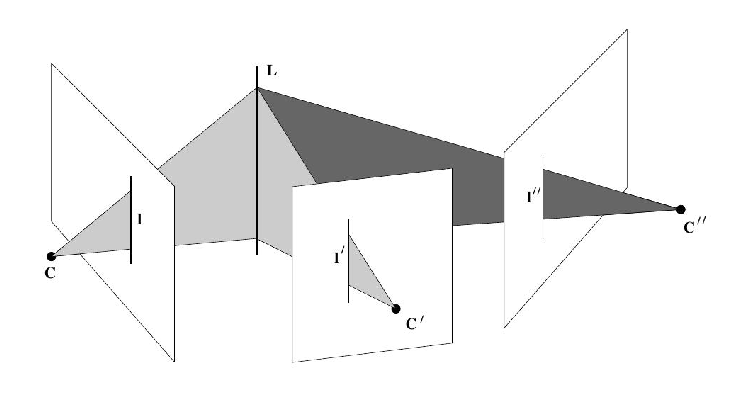
\includegraphics[scale=1]{abord-geo-tri}
\caption{{\it O desenvolvimento algébrico do tensor trifocal realizado a partir das três imagens de uma reta no espaço 3D.}}
\label{fig.abord-geo-tri}
\end{figure}
Considerando $\alpha$, $\beta$ e $k$ escalares, o posto dois de $M$ pode ser interpretado com uma dependência linear entre suas colunas, e como
\begin{equation*}
M=
\begin{bmatrix}
\lightrgb&A^\top\lightrgb'&B^\top\lightrgb''\\
0&{\bf a}^\top_4\lightrgb'&
{\bf b}^\top_4\lightrgb''
\end{bmatrix}
\end{equation*}
podemos definir o sistema
\begin{equation}\label{eq.sistema-tri}
\begin{pmatrix}
\lightrgb\\
0
\end{pmatrix}
=
\alpha
\begin{pmatrix}
A^\top\lightrgb'\\
{\bf a}^\top_4\lightrgb'
\end{pmatrix}
+\beta
\begin{pmatrix}
B^\top\lightrgb''\\
{\bf b}^\top_4\lightrgb''
\end{pmatrix}.
\end{equation}
Pela quarta equação do sistema \ref{eq.sistema-tri} temos
\begin{equation*}
\alpha=k\,{\bf b}^\top_4\lightrgb''\quad\text{e}\quad\beta=-k\,{\bf a}^\top_4\lightrgb'\quad\Rightarrow\quad0=\alpha\,{\bf a}^\top_4\lightrgb'+\beta\,{\bf b}^\top_4\lightrgb''.
\end{equation*}
Substituindo os valores de $\alpha$ e $\beta$ nas três primeiras equações do sistema \ref{eq.sistema-tri} e desconsiderando o fator de escala $k$, temos
\begin{equation*}
\begin{array}{rcl}
\lightrgb&=&\alpha\,A^\top\lightrgb'+\beta\,B^\top\lightrgb''\\
\lightrgb&=&({\bf b}^\top_4\lightrgb'')A^\top\lightrgb'-({\bf a}^\top_4\lightrgb')B^\top\lightrgb''\\
\lightrgb&=&(\lightrgb''^\top{\bf b}_4)A^\top\lightrgb'-(\lightrgb'^\top{\bf a}_4)B^\top\lightrgb''.
\end{array}
\end{equation*}
A $i$-ésima coordenada de $\lightrgb$ pode ser dada por
\begin{equation*}
\begin{array}{rcl}
l_i&=&\lightrgb''^\top({\bf b}_4{\bf a}^\top_i)\lightrgb'-\lightrgb'^\top({\bf a}_4{\bf b}_i^\top)\lightrgb''\\
l_i&=&\lightrgb'^\top({\bf a}_i{\bf b}^\top_4)\lightrgb''-\lightrgb'^\top({\bf a}_4{\bf b}_i^\top)\lightrgb''\\
l_i&=&\lightrgb'^\top({\bf a}_i{\bf b}^\top_4-{\bf a}_4{\bf b}_i^\top)\lightrgb''\\
l_i&=&\lightrgb'^\top \mbox{T}_i\lightrgb'',
\end{array}
\end{equation*}
onde definimos $\mbox{T}_i={\bf a}_i{\bf b}^\top_4-{\bf a}_4{\bf b}_i^\top$. 
O conjunto das três matrizes $\left\{\mbox{T}_1,\mbox{T}_2,\mbox{T}_3\right\}$ é denominado {\it tensor trifocal} e a reta $\lightrgb$ é dada por
\begin{equation}\label{eq.tres-retas}
\lightrgb=
\begin{pmatrix}
\lightrgb'^\top \mbox{T}_1\lightrgb''\\
\lightrgb'^\top \mbox{T}_2\lightrgb''\\
\lightrgb'^\top \mbox{T}_3\lightrgb''
\end{pmatrix}.
\end{equation}

\subsubsection{Homografia induzida por um plano}\label{sec.homo-plano-tri}
Vimos na subseção anterior que podemos determinar o tensor trifocal através da relação entre três retas correspondentes, mas existem mais quatro relações entre retas e pontos  correspondentes envolvendo o tensor trifocal. Para derivarmos essas outras relações e voltarmos ao problema da transferência de pontos, precisamos definir a homografia entre a primeira e terceira imagens induzida por um plano $\bpi'$, retroprojetado por uma reta $\lightrgb'$ na segunda imagem, conforme a figura \ref{fig.transfer-retas}.
\begin{figure}[!htb]
\centering
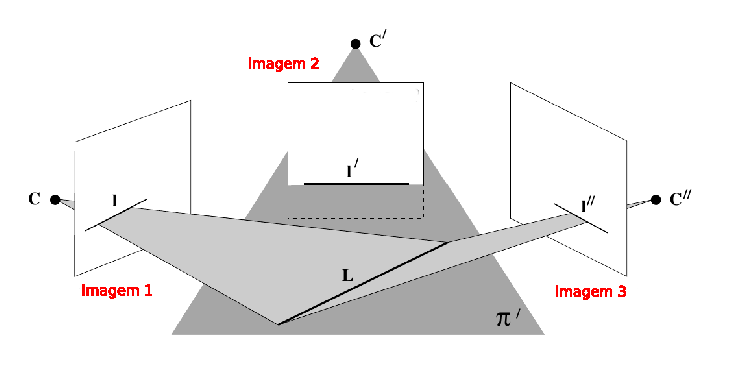
\includegraphics[scale=1]{transfer-retas}
\caption{{\it O plano $\bpi'$ retroprojetado por $\lightrgb'$ induz uma homografia que relaciona $\lightrgb$ com $\lightrgb''$.}}
\label{fig.transfer-retas}
\end{figure}
As homografias entre pontos e retas em dois planos são dadas, respectivamente, por $\x''=H\,\x$ e $\lightrgb''=H^{-\top}\lightrgb$ (subseção \ref{sec.trans-proj-H}). Invertendo $H^{-\top}$ temos que $\lightrgb=H^\top\lightrgb''$. Como temos três retas correspondentes que satizfazem a relação \ref{eq.tres-retas}, podemos comparar essa relação com $\lightrgb=H^\top\lightrgb''$ e deduzir que $H=[\mbox{T}_1^\top\lightrgb',\mbox{T}_2^\top\lightrgb',\mbox{T}_3^\top\lightrgb']$, pois
\begin{equation*}
\lightrgb=
\begin{pmatrix}
\lightrgb'^\top \mbox{T}_1\lightrgb''\\
\lightrgb'^\top \mbox{T}_2\lightrgb''\\
\lightrgb'^\top \mbox{T}_3\lightrgb''
\end{pmatrix}=
\begin{pmatrix}
(\mbox{T}_1^\top\lightrgb')^\top\lightrgb''\\
(\mbox{T}_2^\top\lightrgb')^\top\lightrgb''\\
(\mbox{T}_3^\top\lightrgb')^\top\lightrgb''
\end{pmatrix}=
\begin{pmatrix}
{\bf h}_1^\top\lightrgb''\\
{\bf h}_2^\top\lightrgb''\\
{\bf h}_3^\top\lightrgb''
\end{pmatrix}=
\begin{bmatrix}
{\bf h}_1^\top\\
{\bf h}_2^\top\\
{\bf h}_3^\top
\end{bmatrix}\,\lightrgb''=
H^\top\lightrgb'',
\end{equation*}
onde tomamos ${\bf h}_i=\mbox{T}_i^\top\lightrgb'$.
A homografia deduzida acima (denotada por $H_{13}$) representa a transformação de um ponto da primeira imagem para a terceira através de uma reta na segunda imagem, $\x''=H_{13}\x$. Analogamente, podemos deduzir a homografia da primeira imagem para a segunda através de uma reta na terceira imagem, $\x'=H_{12}\x$.

\subsubsection{Relações de incidência entre pontos e retas}\label{sec.rela-incidi-tri}
Uma das relações de incidência já foi deduzida anteriormente, chamada reta-reta-reta, e agora vamos deduzir mais quatro relações. Supondo ainda $\lightrgb$, $\lightrgb'$ e $\lightrgb''$ três imagens de uma reta ${\bf L}$, sabemos que um ponto $\x$ pertence à uma reta $\lightrgb$ na câmera 1 se $\x^\top\lightrgb=0$, onde a multiplicação matricial pode ser escrita sob a notação de somatório como $\sum_{i=1}^{3}x^il_i=0$. A equação \ref{eq.tres-retas} pode ser dada como $\lightrgb'^\top \mbox{T}_i\lightrgb''
=l_i$ para $i=1,2,3$, e usando o somatório temos que
\begin{equation*}
\begin{array}{rcl}
\lightrgb'^\top \mbox{T}_i\lightrgb''
&=&l_i\\
\sum_{i=1}^3 x^i(\lightrgb'^\top \mbox{T}_i\lightrgb'')&=&\sum_{i=1}^3 x^il_i\\
\lightrgb'^\top(\sum_{i=1}^3 x^i\mbox{T}_i)\lightrgb''&=&0.
\end{array}
\end{equation*}
Desta forma, temos a segunda relação de incidência chamada ponto-reta-reta, para um ponto $\x$ na primeira imagem e as retas $\lightrgb'$ e $\lightrgb''$ na segunda e terceira imagens respectivamente. 

Pela subseção \ref{sec.proj.retas} sabemos da existência de um ponto $\X\in{\bf L}$ que projeta $\x\in\lightrgb$ na primeira imagem e projeta a outros dois pontos $\x'\in\lightrgb'$ e $\x''\in\lightrgb''$, ou seja, temos a correspondência $\x\leftrightarrow\x'\leftrightarrow\x''$. Assim, podemos deduzir as relações para 
pontos na segunda e terceira imagens utilizando a homografia induzida por plano, e vamos tratar da terceira relação de incidência, o caso ponto-reta-ponto. Usando o resultado da subseção \ref{sec.homo-plano-tri} temos que 
\begin{equation*}
\begin{array}{rcl}
\x''&=&H_{13}\x\\
&=&[\mbox{T}_1^\top\lightrgb',\mbox{T}_2^\top\lightrgb',\mbox{T}_3^\top\lightrgb']\x\\
&=&
\begin{pmatrix}
x_1\mbox{T}_1^\top\lightrgb'+x_2\mbox{T}_2^\top\lightrgb'+x_3\mbox{T}_3^\top\lightrgb'
\end{pmatrix}\\
&=&(\sum_{i=1}^3 x^i\mbox{T}_i^\top)\,\lightrgb'
\end{array}
\end{equation*}
Como estamos expressando os vetores em coordenadas homogêneas, essas equações são invariáveis para a aplicação de um fator de escala. De qualquer maneira, podemos eliminar o problema das diferenças de escala aplicando a transposição seguida do produto vetorial à direita em ambos os lados da equação
\begin{equation}\label{eq.ponto-reta-ponto}
\begin{array}{rcl}
\x''&=&(\sum_{i=1}^3 x^i\mbox{T}_i^\top)\,\lightrgb'\\
\x''^\top&=&\lightrgb'^\top(\sum_{i=1}^3 x^i\mbox{T}_i)\\
\x''^\top[\x'']_\times&=&\lightrgb'^\top(\sum_{i=1}^3 x^i\mbox{T}_i)[\x'']_\times\\
{\bf 0}^\top&=&\lightrgb'^\top(\sum_{i=1}^3 x^i\mbox{T}_i)[\x'']_\times.
\end{array}
\end{equation}
O quarto caso, ponto-ponto-reta, é análogo ao apresentado aqui substituindo $\x''$ por $\x'$, e usando a homografia induzida pelo plano retroprojetado por $\lightrgb''$, $\x'=H_{12}\x$.

Por último, temos a relação de incidência para três pontos. 
Observe que a reta $\lightrgb'$ na relação \ref{eq.ponto-reta-ponto} pode ser definida como $\lightrgb'=\x'\times \y'=[\x']_\times \y'$, já que $\x'\in\lightrgb'$ e $\y'$ é um ponto qualquer no plano da segunda imagem. Substituindo $\lightrgb'$, a relação \ref{eq.ponto-reta-ponto} se torna 
\begin{equation*}
\y'^\top[\x']_\times(\sum_{i=1}^3 x^i\mbox{T}_i)[\x'']_\times={\bf 0}^\top,
\end{equation*}
mas observe que tal relação é válida para qualquer reta $\lightrgb'$ que seja imagem de ${\bf L}$, e portanto não depende da escolha do ponto $\y'$ que pode ser descartado. A relação ponto-ponto-ponto é
\begin{equation*}
[\x']_\times(\sum_{i=1}^3 x^i\mbox{T}_i)[\x'']_\times=0_{3\times3}.
\end{equation*}
Cabe resaltar que apenas satisfazer qualquer das relações de incidência não garante a incidência no espaço 3D, ou seja, o tensor trifocal obtido pode não ter consistência com a geometria trifocal de abordagem do problema.

\subsubsection{Relação de incidência para retas epipolares}\label{sec.rela-reta-epipolar-tri}
Suponha que os planos retroprojetados por $\lightrgb$ e $\lightrgb'$ sejam coincidentes e que o ponto 3D $\X$ pertença a esse plano denotado por $\bpi'$, de acordo com a figura \ref{fig.plano-epipolar-tri}. Neste caso, $\bpi'$ é o plano epipolar para as câmeras 1 e 2, e a reta retroprojetada por $\x$, imagem de $\X\in{\bf L}$, está inteiramente contida em $\bpi'$. Como dois planos não coincidentes sempre definem uma reta, o plano retroprojetado por $\lightrgb''$ intersecta o plano $\bpi'$ em ${\bf L}$. Já que a reta retroprojetada por $\x$ está inteiramente contida em $\bpi'$, essa reta deverá intersectar a reta ${\bf L}$ no ponto $\X$. Desta forma, pela subseção \ref{sec.rela-incidi-tri}, temos a correspondência $\x\leftrightarrow\lightrgb'\leftrightarrow\lightrgb''$ que satisfaz a relação
\begin{equation*}
\lightrgb'^\top(\sum_{i=1}^3 x^i\mbox{T}_i)\lightrgb''=0.
\end{equation*}
Observe que, como dois planos sempre definem uma reta, a incidência não depende da escolha do plano retroprojetado pela câmera 3, ou seja, essa incidência vai ocorrer qualquer que seja a reta $\lightrgb''$. Consequentemente, a relação anterior não depende de $\lightrgb''$, e pode ser reduzida a 
\begin{equation}\label{eq.rela-incide-epipolar}
\lightrgb'^\top(\sum_{i=1}^3 x^i\mbox{T}_i)={\bf 0}^\top\quad\text{ou}\quad(\sum_{i=1}^3 x^i\mbox{T}_i)\lightrgb''={\bf 0}.
\end{equation}
A argumentação é análoga considerando o plano epipolar definido pelas retas $\lightrgb$ e $\lightrgb''$, e neste caso a relação será independente da posição da reta $\lightrgb'$. 
\begin{figure}[!htb]
\centering
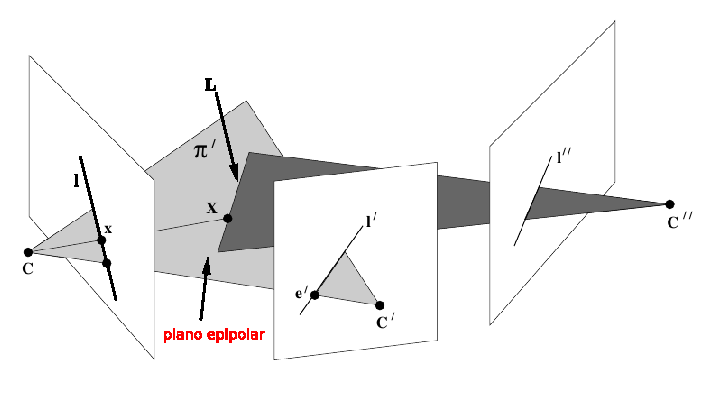
\includegraphics[scale=1]{plano-epipolar-tri}
\caption{{\it Quando ${\bf L}$ pertence a um plano epipolar definido para duas imagens, a relação de incidência $\x\leftrightarrow\lightrgb'\leftrightarrow\lightrgb''$ não depende da reta numa terceira imagem.}}
\label{fig.plano-epipolar-tri}
\end{figure}

Pelas relações em \ref{eq.rela-incide-epipolar} notamos que é possível calcular as retas epipolares como o espaço nulo da matriz $\sum_{i=1}^3 x^i \mbox{T}_i$. Variando o ponto $\x$ é possível obter várias retas epipolares, e todas passam pelo mesmo epipolo. Assim, podemos calcular os epipolos $\e'$ e $\e''$ como interseção dessas retas. Tal resultado será importante na abordagem sobre reconstrução 3D por ocasião da extração das matrizes das câmeras a partir do tensor trifocal.

\subsection{Transferências usando o tensor trifocal}

\subsubsection{Transferência de pontos}
A primeira vantagem no uso do tensor trifocal é que, dos casos de degeneração apresentados na subseção \ref{sec.trans-epipolar}, apenas um deles não pode ser resolvido pelo uso do tensor, como veremos a seguir. 

Considere novamente que se deseja, dada a correspondência entre pontos nas duas primeiras imagens $\x\leftrightarrow\x'$, determinar as coordenadas do ponto correspondente na terceira imagem, $\x''$. Escolhendo uma reta $\lightrgb'$ passando por $\x'$ na segunda imagem e de posse do tensor trifocal, podemos utilizar a relação de incidência 
\begin{equation}\label{eq.ponto-reta-ponto-isolada}
\x''=(\sum_{i=1}^3 x^i\mbox{T}_i^\top)\,\lightrgb'
\end{equation} 
deduzida na subseção \ref{sec.rela-incidi-tri}
para computar diretamente $\x''$. Devemos apenas ter um pouco de cuidado na escoha da reta $\lightrgb'$, pois no caso de ser a reta epipolar correspondente a $\x$ temos, pela subseção \ref{sec.rela-reta-epipolar-tri}, que $(\sum_{i=1}^3 x^i\mbox{T}_i^\top)\,\lightrgb'={\bf 0}$, e o ponto $\x''$ não pode ser determinado. Uma das formas de resolver o problema seria escolher duas ou três retas passando por $\x'$, computar o ponto $\x''$ e escolher aquele que apresenta a maior norma. Outra opção, caso tenha extraído a matriz fundamental $F_{21}$ para as câmeras 1 e 2, é calcular a reta epipolar $\lightrgb'_{\e}=F_{21}\x$ e escolher $\lightrgb'$ que seja perpendicular a $\lightrgb'_{\e}$, ou seja, $\lightrgb'^\top\lightrgb'_{\e}=0$. 

Considere, pela figura \ref{fig.trifocal-frente}, o caso onde o ponto $\X$ está alojado na reta base definida por $\C$ e $\C'$. Nessa posição, a imagem de $\X$ na câmera 2 é o epipolo $\e_{21}=\x'$. Para escolha de qualquer reta que passe por $\x'$ para aplicarmos a relação \ref{eq.ponto-reta-ponto-isolada}, estaremos escolhendo uma reta epipolar, e como vimos anteriormente, não poderemos definir a posição do ponto $\x''$. Tal reta base é o único lugar que $\X$ pode se alojar no plano trifocal que não permite que o ponto $\x''$ seja calculado usando o tensor trifocal, em contraste com a transferência epipolar que se degenera para qualquer $\X$ no plano trifocal. Observe pela figura \ref{fig.X-plano-trifocal} que, desde que a reta ${\bf L}$ não pertença ao plano trifocal, não há motivos para a degeneração da transferência usando o tensor trifocal à medida que variamos a posição de $\X$ em ${\bf L}$. 
\begin{figure}[!htb]
\centering
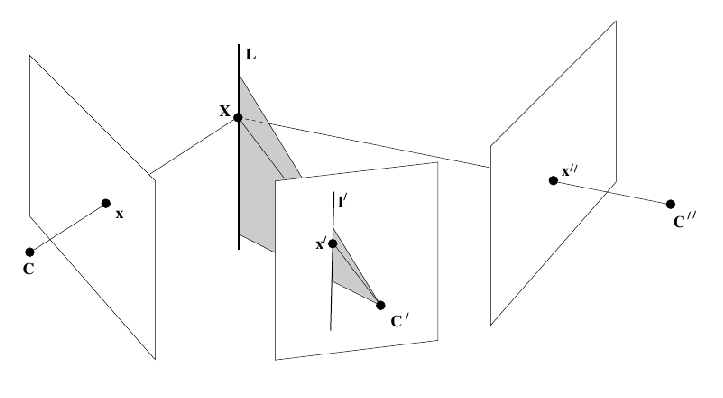
\includegraphics[scale=1]{X-plano-trifocal}
\caption{{\it Desde de que ${\bf L}$ não pertença ao plano trifocal, não há motivos para degenerações à medida que variamos $\X$ em ${\bf L}$.}}
\label{fig.X-plano-trifocal}
\end{figure}
No caso onde os centros das câmeras estão alinhados, não poderemos determinar a posição de $\x''$ caso $\X$ esteja em quaisquer das três retas base, já que assim essas três retas são uma reta só. Lembramos que a transferência epipolar falha para centros de projeção alinhados qualquer que seja a posição de $\X$.  

\subsubsection{Transferência de retas}
Podemos realizar a transferência de retas utilizando a relação
\begin{equation*}
\lightrgb=
\begin{pmatrix}
\lightrgb'^\top \mbox{T}_1\lightrgb''\\
\lightrgb'^\top \mbox{T}_2\lightrgb''\\
\lightrgb'^\top \mbox{T}_3\lightrgb''
\end{pmatrix},
\end{equation*}
que dá uma maneira explícita de calcularmos a reta na primeira imagem dadas as retas nas câmeras 2 e 3. Mas podemos calcular retas em quaisquer das três imagens dadas as outras duas, aplicando o produto vetorial por $\lightrgb$ em ambos os lados da equação
\begin{equation*}
\begin{array}{rcl}
\lightrgb\times\lightrgb&=&\lightrgb\times
\begin{pmatrix}
\lightrgb'^\top \mbox{T}_1\lightrgb''\\
\lightrgb'^\top \mbox{T}_2\lightrgb''\\
\lightrgb'^\top \mbox{T}_3\lightrgb''
\end{pmatrix}\\
{\bf 0}&=&\lightrgb\times
\begin{pmatrix}
\lightrgb'^\top \mbox{T}_1\lightrgb''\\
\lightrgb'^\top \mbox{T}_2\lightrgb''\\
\lightrgb'^\top \mbox{T}_3\lightrgb''
\end{pmatrix}.\\
\end{array}
\end{equation*}
O sistema fornece três equações, sendo duas independentes, para determinar os dois graus de liberdade da reta procurada. Outra vantagem no uso de tensor trifocal é que retas não podem ser determinadas usando apenas matrizes fundamentais.

Repare, pela figura \ref{fig.plano-epipolar-tri}, que se as retas $\lightrgb$ e $\lightrgb'$ retroprojetam o mesmo plano, então não teremos uma única reta definida em 3D que possa ser projetada na terceira imagem, e essas duas retas são retas epipolares correspondentes. Similarmente, não podemos determinar a reta na segunda imagem caso as retas na primeira e terceira imagens sejam retas epipolares correspondentes. Em posições gerais, não há motivo para a geometria epipolar entre as câmeras 1 e 2, e câmeras 1 e 3 serem iguais, ou seja, os dois tipos de transferência não se degeneram simultaneamente com frequência. No entanto, assim como pontos na tranferência epipolar, não é possível aplicar a transferência através do tensor trifocal se a reta 3D estiver contida no plano trifocal. 

\subsection{Reconstrução das câmeras a partir do tensor trifocal}
Assim como foi mostrado no caso bifocal, mostraremos agora como extrair as matrizes fundamentais e as matrizes das câmeras a partir do tensor trifocal.

\subsubsection{Extração da matriz fundamental}\label{sec.extracao-F-tri}
Considerando um ponto $\x$ na primeira imagem, como vimos na subseção \ref{sec.homo-plano-tri}, temos uma homografia que relaciona a primeira com a terceira imagem através de um plano retroprojetado por uma reta $\lightrgb'$ na segunda imagem, conforme a figura \ref{fig.transfer-retas}. Com isso, podemos definir a reta epipolar $\lightrgb''$ na terceira imagem relativa ao ponto $\x$ na primeira imagem. O ponto $\x''$ na terceira imagem é dado por
\begin{equation*}
\x''=H_{13}\x\quad\text{ou}\quad\x''=[\mbox{T}_1^\top\lightrgb',\mbox{T}_2^\top\lightrgb',\mbox{T}_3^\top\lightrgb']\,\x,
\end{equation*}  
e a reta epipolar na terceira imagem pode ser calculada como $\lightrgb''=\e''\times\x''$. Substituindo a expressão para $\x''$ temos
\begin{equation*}
\begin{array}{rcl}
\lightrgb''&=&\e''\times\x''\\
\lightrgb''&=&[\e'']_\times[\mbox{T}_1^\top\lightrgb',\mbox{T}_2^\top\lightrgb',\mbox{T}_3^\top\lightrgb']\,\x\\
\lightrgb''&=&F_{31}\,\x,
\end{array}
\end{equation*}
onde a matriz fundamental pode ser obtida por $F_{31}=[\e'']_\times[\mbox{T}_1^\top\lightrgb',\mbox{T}_2^\top\lightrgb',\mbox{T}_3^\top\lightrgb']$.

Algebricamente esta expressão se mantém para qualquer reta $\lightrgb'$, mas devemos escolher uma reta para evitar a condição de degeneração onde $\mbox{T}^\top_i\lightrgb'={\bf 0}$. Uma boa escolha é tomar $\lightrgb'=\e'$ pois $\e'$ é perpendicular ao espaço nulo à direita de cada $\mbox{T}^\top_i$. Assim , a matriz fundamental é obtida simplesmente por
\begin{equation*}
F_{31}=[\e'']_\times[\mbox{T}_1^\top\e',\mbox{T}_2^\top\e',\mbox{T}_3^\top\e'].
\end{equation*} 
Uma análise similar permite verificar que podemos obter uma relação que envolve a segunda e primeira imagens,
\begin{equation*}
F_{21}=[\e']_\times[\mbox{T}_1\e'',	\mbox{T}_2\e'',\mbox{T}_3\e''].
\end{equation*}

\subsubsection{Extraindo as matrizes das câmeras}

Da mesma forma que acontece no caso bifocal, por conta da ambiguidade projetiva, podemos determinar as matrizes das câmeras tomando a câmera 1 como $P=[I|{\bf 0}]$ aplicando uma transformação projetiva. Seguindo a subseção \ref{sec.cameras-canonicas}, dadas duas câmeras $P=[I|{\bf 0}]$ e $P'=[M|{\bf m}]$, a matriz fundamental é extraída como $F=[{\bf m}]_\times M$. Usando a matriz fundamental $F_{21}=[\e']_\times[\mbox{T}_1\e'',	\mbox{T}_2\e'',\mbox{T}_3\e'']$ extraída do tensor trifocal na subseção \ref{sec.extracao-F-tri}, temos que o par de câmeras, dado o tensor trifocal é
\begin{equation}\label{eq.deducao-simples-P-tri}
P=[I|{\bf 0}]\quad\text{e}\quad P'=[[\mbox{T}_1\e'',\mbox{T}_2\e'',\mbox{T}_3\e'']|\e'].
\end{equation}

Poderíamos pensar que as câmeras 1 e 3 poderiam ser obtidas usando a matriz fundamental $F_{31}=[\e'']_\times[\mbox{T}_1^\top\e',\mbox{T}_2^\top\e',\mbox{T}_3^\top\e']$, e daí a câmera 3 seria $P''=[[\mbox{T}_1^\top\e',\mbox{T}_2^\top\e',\mbox{T}_3^\top\e']|\e'']$, mas está {\it incorreto}. A câmera 3 não pode ser escolhida independentemente das características projetivas das câmeras 1 e 2. Pois, observe que podemos reconstruir o ponto 3D $\X$ a partir das câmeras 1 e 2, e usá-lo para determinar a câmera 3 usando as correspondências $\X\leftrightarrow\x''$, conforme o artigo na seção \ref{sec.astrom}. Assim, $P''$ depende das características projetivas do par $(P,P')$. 

De acordo com a subseção \ref{sec.ambi-cameras-dada-F} e usando a dedução dada pela equação \ref{eq.deducao-simples-P-tri}, uma forma mais geral de se obter $P$ e $P'$ é dada por
\begin{equation}\label{eq.familia-cameras}
P=[I|{\bf 0}]\quad\text{e}\quad P'=[[\mbox{T}_1\e'',\mbox{T}_2\e'',\mbox{T}_3\e'']+\e'^\top{\bf v} |\lambda\,\e'],
\end{equation}    
para algum vetor ${\bf v}$ e um escalar $\lambda$. E para determinarmos $P''$ devemos obter um trio de câmeras dessa família que seja compatível com a dedução do tensor trifocal dada na subseção \ref{sec.tensor-tri-rela-inci},
\begin{equation}\label{eq.tensor-tri}
\mbox{T}_i={\bf a}_i{\bf b}_4^\top-{\bf a}_4{\bf b}_i^\top,
\end{equation}
onde ${\bf a}_i$ são a colunas de $P'$ e ${\bf b}_i$ são as colunas de $P''$.
Por conta da ambiguidade projetiva, dentre essa família de câmeras em \ref{eq.familia-cameras}, podemos escolher $P'=[[\mbox{T}_1\e'',\mbox{T}_2\e'',\mbox{T}_3\e'']|\e']$ para desta forma termos ${\bf a}_i=\mbox{T}_i\e''$ para $i=$1,2 e 3. Notando que ${\bf a}_4=\e'$ e ${\bf b}_4=\e''$, podemos substituir as três últimas relações na equação \ref{eq.tensor-tri} e obter
\begin{equation*}
\mbox{T}_i=\mbox{T}_i\e''\e''^\top-\e'{\bf b}_i^\top,
\end{equation*}
onde, isolando ${\bf b}_i^\top$ temos 
\begin{equation}\label{eq.deri-parcial-P''}
\e'{\bf b}_i^\top=\mbox{T}_i (\e''\e''^\top-I)
\end{equation}
Como o fator de escala é irrelevante, podemos escolher $\e'$ de forma que $\e'^\top\e'=1$, multiplicar $\e'^\top$ pela esquerda na relação \ref{eq.deri-parcial-P''} e aplicar a transposta para chegarmos a
\begin{equation*}
{\bf b}_i=(\e''\e''^\top -I)\mbox{T}_i^\top\e'.
\end{equation*}
Agora podemos definir a câmera 3 considerando as características projetivas das câmeras 1 e 2,
\begin{equation*}
P''=[(\e''\e''^\top -I)[\mbox{T}_1^\top\e',\mbox{T}_2^\top\e',\mbox{T}_3^\top\e']|\e''],
\end{equation*}
e assim verificarmos que o tensor trifocal determina completamente as matrizes das câmeras a menos de uma ambiguidade projetiva.


\section{Geometria Diferencial Trifocal}

\subsection{Abordagem do Fabbri}
Problema 2.

\subsection{Nova Solução}

\subsection{Novo Algoritmo}

\subsection{Experimentos com novo Algoritmo}



\section{Aplicações da Geometria Diferencial Trifocal}\label{sec:apli:geo:dif:tri}
(Objetivo: apanhado geral do uso de geometria trifocal e ideias novas)

\subsection{Aplicações em Sistemas de SfM}
Aplicações em structure for motion.

Explicar como utilizar os resultados dos dois últimos capítulos em sistema real.

\subsection{Outras Aplicações}

\section{Experimentos}
\section{Conclusões}
\nocite{Fabbri:Kimia:CVPR10,Hartley2004,Faugeras,Schmid00,2503343,HartleyLi,koser,kukelova,pajdla,byrod}


\appendix
\section{Possiveis Publicacoes}
\subsection{Trifocal Relative Pose using First-Order Differential Geometry}
Paper mais importante onde resolveriamos o problema para pontos e tangentes.

Capitulos de tese: \ref{sec:geo:dif:tri}

\subsection{Using Trifocal Geometry in Structure from Motion}
Outros titulos:
"Trifocal geometry: Theory and practice in real SfM systems"
"Exploiting Trifocal geometry for bootstrapping SfM systems"
"A Survey of Trifocal Geometry in Structure from Motion"

Capitulos de tese: \ref{sec:apli:geo:dif:tri}

Este responderia às seguintes perguntas:
Qual a vantagem de se iniciar um sistema de autocalibracao externa de cameras usando
geometria trifocal?  O que se ganha em reconstrucao/estereo?

Experimentos:
- implementar bundler com geometria trifocal e observar melhorias
	
\bibliographystyle{plainnat} 
\bibliography{biblio}
\end{document}
